\documentclass[oneside,envcountsame,envcountchap,openany]{svmono}

% Pacotes de referências e bibliografia
\usepackage[backend=biber, style=numeric, url=true, sorting=ynt]{biblatex}
\DefineBibliographyStrings{portuguese}{
  urlseen = {Consultado em}
}
\addbibresource{referencias.bib}


% Pacotes de formatação e layout
\usepackage[top=1in,left=1.5in,bottom=1in,right=2.5cm]{geometry}
\usepackage{fancyhdr}
\usepackage{makeidx}         % permite geracao de indice
\usepackage{graphicx}        % ferramenta padrao latex
\usepackage{multicol}        % usada para fazer múltiplas colunas
\usepackage[bottom]{footmisc}% coloca rodapés no final da página
\usepackage{placeins}		 % para forçar o float a ficar na seção
\usepackage{pdfpages}		 % para incluir pdfs
\usepackage{tocloft} 		 % para formatar o sumário
\setlength\cftparskip{-2pt}
\setlength\cftbeforechapskip{0pt}
\usepackage[titletoc,toc,page]{appendix} % para anexos
\usepackage{scrextend}		 % para adicionar margens
\usepackage{quoting}		% para citações
\quotingsetup{leftmargin=2em, rightmargin=2em, font=itshape}

% Pacotes de tabelas e cores
\usepackage[table]{xcolor}  % para tabelas coloridas
\usepackage{tabularx}		% para tabelas com largura automática
\usepackage{longtable}		% para tabelas longas
\usepackage{spreadtab}	    % para tabelas com cálculos
\usepackage{booktabs}		% para tabelas com linhas horizontais
\usepackage{multirow}		 % para tabelas com multiplas linhas
\usepackage{caption}
\captionsetup{labelfont=bf, font=small, textfont=small}  % Força o negrito somente no "Tabela x:"
\renewcommand{\arraystretch}{1.5}


% Pacotes de texto e fontes
\usepackage[T1]{fontenc} 	% para acentuação correta
\usepackage[portuguese]{babel} % para português
\usepackage{enumerate}		% para listas enumeradas
\usepackage{textcomp}		% para símbolos de texto
\usepackage{xspace}			% para espaçamento automático

% Pacotes de gráficos e desenhos
\usepackage{tikz}			% para gráficos e desenhos
\usetikzlibrary{calc}		% para cálculos em gráficos

% Pacote para posicionamento de texto
\usepackage[absolute]{textpos}

% Pacotes de hiperlinks
\usepackage{hyperref}
\hypersetup{
	colorlinks,
	citecolor=blue,
	filecolor=magenta,
	linkcolor=black, % Changed from red to black for better readability
	urlcolor=cyan
}

% Configuração de cabeçalhos e rodapés
\pagestyle{fancy}
\fancyhf{} % limpa cabeçalho e rodapé
\fancyhead[R]{\footnotesize  \thepage} % número de página no topo à direita
\fancyhead[L]{\footnotesize \nouppercase{\leftmark}} % nome do capítulo no topo à esquerda
\renewcommand{\headrule}{} 
\fancyfoot{}
\addtolength{\headwidth}{0.3\marginparwidth}
\setlength{\headheight}{15pt}

% Redefinimos o estilo plain, usado no sumário
\fancypagestyle{plain}{
  \fancyhf{}
  \renewcommand{\headrulewidth}{0pt}
  \fancyhead[R]{\footnotesize \thepage}  
}

% Configuração de índices e listas
\makeindex             % para gerar índice

% Configuração de anexos
\renewcommand{\appendixtocname}{Anexos}
\renewcommand{\appendixpagename}{Anexos}

% Definição de comandos personalizados
% Definição de ordinal masculino e feminino
\usepackage{etoolbox} % para garantir compatibilidade em várias situações

\DeclareRobustCommand{\subsup}[1]{%
  \textsuperscript{%
    \tikz[baseline=(char.base)]{
      \node[inner sep=0.5pt, anchor=base] (char) {\textnormal{#1}};
      \draw[line width=0.3pt, yshift=-0.2ex]
        ($(char.south west)!0.15!(char.south east)$) --
        ($(char.south west)!0.85!(char.south east)$);
    }%
  }%
}

\DeclareRobustCommand{\ordm}[1]{#1\subsup{o}} % ordinal masculino
\DeclareRobustCommand{\ordf}[1]{#1\subsup{a}} % ordinal feminino

\newenvironment{itquotation}
{\begin{quotation}
  \itshape % itálico
  }
{\end{quotation}}	
% No paragraph indentation
\parindent0pt
\setlength{\parskip}{0.8\baselineskip}

% Nomes das Disciplinas
\usepackage{./disciplinasDB} % Ensure the file disciplinasDB.sty is in the same directory as this .tex file

\normalsize %define o tamanho da fonte como normal

\newcommand{\desc}{Departamento de Engenharia de Sistemas e Computação\xspace}

% ********************** Início do documento ***********************************
\begin{document}
%\author {Departamento de Engenharia de Sistemas e Computação}
% Definição de créditos, horas, etc....
% NAO EDITE MANUALMENTE
% Este arquivo foi gerado automaticamente em 2025-5-12
% MACROS CRIADAS
% 1. tHorasCurso: Total de horas do curso: 
% 2. hTotaisDisc: Total de horas de disciplinas (regulares+eletivas+extensao): 
% 3. hTotaisDiscObrigComDiscExt: Total de horas de disciplinas obrigatórias (regulares+extensao)
% 4. hDiscObrigSemExtensao: Total de horas de disciplinas obrigatórias sem extensão
% 5. tHorasSemExtensao: Total de horas de Disc obrig sem extensao
% 6. hDiscExtensao: Total de horas de disciplinas de extensão
% 7. hExtensao: Total de horas de extensão
% 8. hACE Total de horas de atividades de extensão (sem disciplinas)
% 9. nEletivas: Número de disciplinas eletivas
% 10. credEletivas: Total de créditos de disciplinas eletivas
% 11. tCredCurso: Total de créditos do curso
% 12. credObrigSemExtensao: Total de créditos de disciplinas obrigatórias sem extensão
% 13. hEletivas: Total de horas de disciplinas eletivas
% 14. credDiscExtensao: Total de créditos disciplinas de extensao
% 15. nDisciplinas: Número total de disciplinas
% 16. nDiscObrigatorias: Número de disciplinas obrigatorias
\RequirePackage{siunitx}
\sisetup{ group-separator = {.}, group-minimum-digits = 4, output-decimal-marker={,}, }
\newcounter {thorasCursoCounter}
\setcounter {thorasCursoCounter}{3501}
\newcounter {hExtensaoCounter}
\setcounter {hExtensaoCounter}{351}
\newcommand {\tHorasCurso}{3501\xspace }
\newcommand {\hTotaisDisc}{\num{3345}\xspace }
\newcommand {\hTotaisDiscObrigComDiscExt}{\num{3225}\xspace }
\newcommand {\tHorasSemExtensao}{3150\xspace }
\newcommand {\hDiscObrigSemExtensao}{3030\xspace }
\newcommand {\hDiscExtensao}{195\xspace }
\newcommand {\hExtensao}{351\xspace }
\newcommand {\hACE}{156\xspace }
\newcommand {\nEletivas}{2\xspace }
\newcommand {\credEletivas}{8\xspace }
\newcommand {\hEletivas}{120\xspace }
\newcommand {\tCredCurso}{223\xspace }
\newcommand {\credObrigSemExtensao}{202\xspace }
\newcommand {\credDiscExtensao}{13\xspace }
\newcommand {\nDisciplinas}{55\xspace }
\newcommand {\nDiscObrigatorias}{53\xspace }

 % Arquivo com os dados do curso

% ======== CAPA ================
\begin{textblock*}{3cm}[0.5,0.5](4cm,4cm)
  
\includegraphics[width=3cm]{imagens/logo_uerj_cor.jpg}
\end{textblock*}
\begin{textblock*}{12cm}(6cm,3cm)   % 6.375=8.5 - 1.5 - 0.625
  Universidade do Estado do Rio de Janeiro\\
  Sub-Reitoria de Graduação \\
  Faculdade de Engenharia\\
  Departamento de Engenharia de Sistemas e Computação
\end{textblock*}

\title{Projeto Pedagógico do Curso de Engenharia de Computação}
\subtitle{2025}
\date{} % sem data
\maketitle
\vfill
\thispagestyle{empty} % Remove número da página
\newpage

% ======= Página com nomes institucionais (sem número)
{\textbf{Reitora}} \\
Gulnar Azevedo e Silva


  {\textbf{Vice-Reitor}} \\
Bruno Rêgo Deusdará Rodrigues

  {\textbf{Pró-Reitor de Graduação}} \\
Antonio Soares da Silva

  {\textbf{Diretora do Centro de Tecnologia e Ciência}} \\
Nádia Pimenta Lima

  {\textbf{Diretora da Faculdade de Engenharia}} \\
Maria Eugenia de las Mercedes Mosconi de Gouvêa

{\textbf{Chefe do Departamento de Engenharia de Sistemas e Computação}} \\
João Araujo Ribeiro

\newpage

% ============= Sumário com estilo isolado
\pagenumbering{roman}
\tableofcontents
\listoftables
\clearpage

\frontmatter%%%%%%%%%%%%%%%%%%%%%%%%%%%%%%%%%%%%%%%%%%%%%%%%%%%%%%

\mainmatter%%%%%%%%%%%%%%%%%%%%%%%%%%%%%%%%%%%%%%%%%%%%%%%%%%%%%%%

% ======== Capítulos ================
\clearpage
\pagestyle{fancy}
% Capítulo: Introdução
\chapter{Introdução}
\label{intro} % Always give a unique label
% use \chaptermark{}
% to alter or adjust the chapter heading in the running head

Este documento apresenta o projeto da estrutura curricular do novo curso de Engenharia de Computação da Universidade do Estado do Rio de Janeiro. Este curso será oferecido pelo Departamento de Engenharia de Sistemas e Computação (DESC) da Faculdade de Engenharia (FEN). Desde 1977, o DESC oferece o curso de Engenharia Elétrica com Ênfase em Sistemas e Computação, sendo o primeiro no Brasil a oferecer uma graduação na área de Engenharia de Computação. O curso passou por uma reformulação significativa no início da década de 1990 e, desde então, manteve o mesmo currículo, sem alterações. O objetivo agora é promover uma reforma deste curso e oferecê-lo como uma nova habilitação em engenharia.

A Engenharia, especialmente a Engenharia de Computação, tem evoluído a passos largos no cenário contemporâneo. Com mais de três décadas desde a última atualização curricular, torna-se imperativo adaptar o curso às exigências atuais, alinhando-o com as demandas da sociedade por avanços científicos e tecnológicos nos setores industrial e de serviços. Atualmente, em 2024, os candidatos aos cursos da Faculdade de Engenharia da UERJ, incluindo a Engenharia Elétrica, enfrentam um dilema. Ao optarem pela Engenharia Elétrica com Ênfase em Sistemas e Computação, recebem um diploma de Engenheiro Eletricista, uma designação que não reflete adequadamente a especialização adquirida, especialmente considerando a necessidade crescente de conhecimentos aprofundados em desenvolvimento de sistemas e dispositivos computacionais, conforme orientado pelas diretrizes do ENADE.

A proposta de introduzir o curso de \textbf{Engenharia de Computação} como uma nova habilitação visa não apenas modernizar o currículo em resposta às transformações tecnológicas, mas também proporcionar uma formação mais alinhada com as competências exigidas no campo da computação. O atual curso de Engenharia Elétrica com Ênfase em Sistemas e Computação, embora prepare os alunos para desenvolver software e projetar hardware, não os capacita adequadamente para projetar sistemas de potência, uma expectativa comum para engenheiros eletricistas. Essa discrepância tem levado a dificuldades para os alunos no ENADE, evidenciando a lacuna entre a formação oferecida e as competências específicas requeridas na área elétrica.

Portanto, a criação de um curso dedicado à Engenharia de Computação, como uma habilitação distinta, é uma resposta estratégica às necessidades educacionais emergentes, garantindo que os egressos estejam melhor preparados para enfrentar os desafios tecnológicos do futuro. Este projeto pedagógico não apenas reflete uma atualização necessária diante das mudanças tecnológicas desde os anos 1990, mas também reafirma o compromisso da UERJ com a excelência educacional e a inovação no ensino de engenharia.

% Capítulo: Dados da Unidade Acadêmica
\chapter{Dados Gerais da Unidade Acadêmica - \textcolor{red}{Rafaela}}


\section{Identificação Geral}

A instituição de educação superior mantenedora do curso de Engenharia de Computação é a Universidade do Estado do Rio de Janeiro que exercerá, por meio da Pró-reitoria de Graduação, a administração acadêmica do curso.

A Universidade do Estado do Rio de Janeiro é organizada em: Administração Central, Centros Setoriais, Unidades Acadêmicas e Departamentos. Todos estão diretamente ligados à Reitoria, por meio de órgãos de assessoria que são: Vice-reitoria, Pró-reitoria de Graduação, Pró-reitoria de Pós-graduação e Pesquisa, Pró-reitoria de Extensão e Cultura, Pró-reitoria de Políticas e Assistência Estudantis, Pró-reitoria de Saúde e a Superintendência de Gestão de Pessoas.


\begin{description}
	\item[Mantenedor:] Governo do Estado do Rio de Janeiro.
	\item [Mantida:] Faculdade de Engenharia -- Universidade do Estado do Rio de Janeiro.
	\item [Local de Funcionamento:] Rua São Francisco Xavier 524, 5$^{o}$ andar, Maracanã, Rio de Janeiro -- RJ.
	\item [Reitora:] Gulnar Azevedo e Silva.
	\item [Vice-Reitor:] Bruno Rêgo Deusdará Rodrigues.
	\item [Pró-Reitor de Graduação (PR1):] Antonio Soares da Silva.
	\item [Pró-Reitora de Pós-graduação e Pesquisa (PR2):] Elizabeth Fernandes de Macedo.
	\item [Pró-Reitora de Extensão e Cultura (PR3):] Ana Maria de Almeida Santiago.
	\item [Pró-Reitora de Políticas e Assistência Estudantis (PR4):] Daniel Pinha Silva.
	\item [Pró-Reitora de Saúde (PR5):] Ronaldo Damião.
	\item [Diretora do Centro de Tecnologia e Ciências:] Nádia Pimenta Lima.
	\item [Diretora da Faculdade de Engenharia:]  Maria Eugênia Gouvêa.
	\item [Chefe do Depto. de Eng. de Sistemas e Computação:]  \araujo.
\end{description}

\subsection{Centro de Vinculação}

Na Universidade do Estado do Rio de Janeiro existem quatro Centros Setoriais: Centro Biomédico, Centro de Ciências Sociais, Centro de Educação e Humanidades e Centro de Tecnologia e Ciências.

O curso de Engenharia de Computação está vinculado ao Centro de Tecnologia e Ciências (CTC).
O CTC é um órgão com função deliberativa e executiva destinado a coordenar e integrar as atividades afins de ensino, pesquisa e extensão nas suas áreas de atuação. Coordena 11 unidades acadêmicas e atualmente possui 732 docentes efetivos o que corresponde a 26\% dos docentes da UERJ. Destes, 83\% possuem título de doutor. Conta com 258 técnico-administrativos e 8506 alunos ativos de graduação e pós-graduação. Congrega 20 cursos de graduação e 27 cursos de pós-graduação. As unidades acadêmicas ligadas ao CTC são as seguintes:

\begin{itemize}

	\item Escola Superior de Desenho Industrial -- ESDI
	\item Faculdade de Ciências Exatas e Engenharias -- FCEE
	\item Faculdade de Engenharia -- FEN
	\item Faculdade de Geologia -- FGEL
	\item Faculdade de Oceanografia -- FAOC
	\item Faculdade de Tecnologia -- FAT
	\item Instituto de Física Armando Dias Tavares -- IFADT
	\item Instituto de Geografia -- IGEOG
	\item Instituto de Matemática e Estatística -- IME
	\item Instituto Politécnico -- IPRJ
	\item Instituto de Química -- QUI

\end{itemize}

\section{Identificação da Unidade Acadêmica}

A Faculdade de Engenharia (FEN) é uma unidade do Centro de Tecnologia e Ciências que oferece na graduação as habilitações de Engenharia Elétrica, Civil, Sanitária e Ambiental, Mecânica, de Produção, Cartográfica, além dos cursos de pós-graduação em níveis lato sensu e stricto sensu, não listados.

A Faculdade de Engenharia é constituída por nove departamentos, com representação no Conselho Departamental:

\begin{itemize}
	\item Departamento de Engenharia Cartográfica -- CARTO
	\item Departamento de Construção Civil e Transportes -- DCCT
	\item Departamento de Engenharia Elétrica -- DEE
	\item Departamento de Eletrônica e Telecomunicações -- DETEL
	\item Departamento de Estruturas e Fundações -- ESTR
	\item Departamento de Engenharia Mecânica -- MECAN
	\item Departamento de Engenharia Industrial -- DEIN
	\item Departamento de Engenharia Sanitária e Meio Ambiente -- DESMA
	\item Departamento de Engenharia de Sistemas e Computação -- DESC
\end{itemize}

A Tabela~\ref{tabvagas} apresenta as vagas atualmente oferecidas para o vestibular pela Faculdade de Engenharia da Universidade do Estado do Rio de Janeiro, campus Maracanã, para o primeiro e para o segundo semestre.
\begin{table}
	\centering
	\caption{Vagas oferecidas no 1\textordmasculine{} e no 2\textordmasculine{} semestre}
	\label{tabvagas}
	\begin{tabularx}{\textwidth}{|X|c|c|c|c|}
		\hline
		\multirow{2}{*}{\textbf{Habilitação}}                 & \multirow{2}{*}{\textbf{Turno}} & \multicolumn{2}{c|}{\textbf{Vagas}} & \multirow{2}{*}{\textbf{Total}}          \\
		\cline{3-4}                                           &                                 & \textbf{1\textordmasculine{} Sem.}  & \textbf{2\textordmasculine{} Sem.} &     \\
		\hline
		Engenharia Ambiental e Sanitária                      & Manhã/Tarde                     & 40                                  & --                                 &     \\
		                                                      & Tarde/Noite                     & --                                  & 40                                 & 80  \\
		\hline
		Engenharia Cartográfica                               & Manhã/Tarde                     & 20                                  & --                                 &     \\
		                                                      & Tarde/Noite                     & --                                  & 20                                 & 40  \\
		\hline
		Engenharia Civil                                      & Manhã/Tarde                     & 60                                  & --                                 &     \\
		(Construção Civil/Transportes/Estruturas)             & Tarde/Noite                     & --                                  & 60                                 & 120 \\
		\hline
		Engenharia de Produção                                & Manhã/Tarde                     & 40                                  & --                                 &     \\
		                                                      & Tarde/Noite                     & --                                  & 40                                 & 80  \\
		\hline
		Engenharia Elétrica (Sistemas e Computação/           & Manhã/Tarde                     & 100                                 & --                                 &     \\
		Sist. de Potência/Sist. Eletrônicos/Telecomunicações) & Tarde/Noite                     & --                                  & 100                                & 200 \\
		\hline
		Engenharia Mecânica                                   & Manhã/Tarde                     & 40                                  & --                                 &     \\
		                                                      & Tarde/Noite                     & --                                  & 40                                 & 80  \\
		\hline
	\end{tabularx}
\end{table}


% Capítulo: Bases Legais
\chapter{Bases Legais}

A reforma curricular do curso de Engenharia de Computação da UERJ foi concebida em consonância com as principais normativas que regem a formação superior na área da Computação e o exercício da profissão de engenheiro no Brasil. Fundamenta-se, principalmente, na Resolução CNE/CES n\textsuperscript{o} 5/2016, que estabelece as Diretrizes Curriculares Nacionais para os cursos de graduação da área, abrangendo os bacharelados em Ciência da Computação, Sistemas de Informação, \textbf{Engenharia de Computação}, Engenharia de Software e a licenciatura em Computação. Essa resolução define os princípios orientadores e os parâmetros estruturais para a organização curricular desses cursos.

Adicionalmente, a proposta considera os \textit{Referenciais de Formação para os Cursos de Graduação em Computação}, publicados em 2017 pela Sociedade Brasileira de Computação (SBC), os quais detalham diretrizes específicas para a formação nas diversas áreas da Computação. Esses referenciais foram elaborados com base na Resolução n\textsuperscript{o} 5/2016, citada anteriormente, oferecendo uma interpretação consolidada e atualizada das competências e conteúdos curriculares esperados, com ênfase nas transformações tecnológicas e nas demandas sociais contemporâneas.

A proposta incorpora ainda os preceitos da Resolução n\textsuperscript{o} 7/2018, do Conselho Nacional de Educação, que dispõe sobre as Diretrizes para a Extensão na Educação Superior Brasileira, em conformidade com a Meta 12.7 da Lei n\textsuperscript{o} 13.005/2014, que institui o Plano Nacional de Educação (PNE) para o período 2014--2024. Essa normativa orienta as instituições de ensino superior a integrarem, de forma indissociável, ensino, pesquisa e extensão, promovendo a formação integral dos estudantes e o fortalecimento dos vínculos com a sociedade.

Do ponto de vista da regulamentação profissional, considera-se a Resolução n\textsuperscript{o} 380 do Conselho Federal de Engenharia e Agronomia, de 17 de dezembro de 1993, que discrimina as atribuições profissionais dos Engenheiros de Computação.

A observância a essas diretrizes assegura a aderência da proposta curricular às normativas nacionais vigentes, bem como sua adequação às exigências contemporâneas da formação profissional e do mercado de trabalho. Busca-se, assim, consolidar uma formação ampla, sólida e atualizada, alinhada às competências requeridas para o exercício da Engenharia de Computação nos âmbitos acadêmico, científico e tecnológico.

A documentação relevante para este processo de reforma curricular está anexada nas páginas seguintes:

\begin{enumerate}
    \item \textbf{Câmara de Educação Superior do Conselho Nacional de Educação}  \\
          \textbf{RESOLUÇÃO CNE/CES N\textsuperscript{o} 5, DE 16 DE NOVEMBRO DE 2016}  \\
          Institui as Diretrizes Curriculares Nacionais para os cursos de graduação na área da Computação, abrangendo os cursos de bacharelado em Ciência da Computação, em Sistemas de Informação, em \textbf{Engenharia de Computação}, em Engenharia de Software e de licenciatura em Computação, e dá outras providências (Anexo \ref{cne2016}).

    \item \textbf{Sociedade Brasileira de Computação (SBC)}  \\
          \textbf{Referenciais de Formação para os Cursos de Graduação em Computação –-- 2017} \\
          Documento elaborado com base na Resolução CNE/CES n\textsuperscript{o} 5/2016, com o objetivo de orientar a estrutura curricular dos cursos da área de Computação, considerando competências, conteúdos e práticas pedagógicas atualizadas (Anexo \ref{sbc2017}).

    \item \textbf{Câmara de Educação Superior do Conselho Nacional de Educação}  \\
          \textbf{RESOLUÇÃO N\textsuperscript{o} 7, DE 18 DE DEZEMBRO DE 2018}  \\
          Estabelece as Diretrizes para a Extensão na Educação Superior Brasileira e regimenta o disposto na Meta 12.7 da Lei n\textsuperscript{o} 13.005/2014, que aprova o Plano Nacional de Educação –-- PNE –-- 2014-2024 e dá outras providências (Anexo \ref{rcne2018}).

    \item \textbf{CONFEA – Conselho Federal de Engenharia e Agronomia} \\
          \textbf{RESOLUÇÃO N\textsuperscript{o} 380, DE 17 DE DEZEMBRO DE 1993}  \\
          Discrimina as atribuições provisórias dos Engenheiros de Computação ou Engenheiros Eletricistas com ênfase em Computação e dá outras providências. Brasília: Diário Oficial da União, Seção I, página 193, 06 de janeiro de 1994 (Anexo \ref{confea1993}).
\end{enumerate}


\section{Normas Gerais de Ensino de Graduação da UERJ}

O funcionamento do curso obedecerá às Normas Gerais de Ensino de Graduação da UERJ definidas pela Deliberação N\textsuperscript{o} 33/95 da UERJ. Seus aspectos principais são apresentados a seguir:

\subsection{Período de integralização do curso}
\begin{quoting}
    Art. 99 –-- Somente receberá o diploma o aluno que cumprir a Integralização Curricular.
\end{quoting}

O período mínimo de integralização curricular dos cursos de Engenharia é de 10 (dez) semestres e o prazo máximo é de 18 (dezoito) semestres (Seção \ref{sec:integralizacao}).

\subsection{Relação entre crédito e carga horária}
Nova redação dada pela Deliberação \ordm{N} 59/2019
\begin{quoting}
    Art. 57 –- O número mínimo de créditos necessários para integralizar o
    currículo será estabelecido com base na carga horária total do curso.


    \S \ordm{1} - Nos cursos de regime de crédito, a unidade padrão de crédito
    corresponde a 15 (quinze) horas, e as atividades de que trata o caput do
    presente artigo são:
    \begin{itemize}
        \item[a)] Aula teórica;
        \item[b)] Trabalho de campo;
        \item[c)] Laboratório/aula prática;
        \item[d)] Estágio curricular;
        \item[e)] Prática como componente curricular.
    \end{itemize}

    \S \ordm{2} - Fica a critério de cada unidade acadêmica determinar a carga horária de  cada atividade/disciplina prevista no \S\ordm{1} deste artigo, de acordo com o Projeto Pedagógico de cada curso, respeitando-se o padrão de 01 (um) crédito para cada 15 (quinze) horas/aula e seus múltiplos.
\end{quoting}
\subsection{Aproveitamento escolar}
\begin{quoting}
    Art. 95 –-- A aprovação do aluno em disciplinas do Curso de Graduação desta Universidade terá por base notas e freqüência. São condições para aprovação: obtenção de nota final mínima 5,0 (cinco vírgula zero), constituída pela média aritmética da média semestral e nota da prova final; freqüência mínima de 75\% (setenta e cinco por cento) do total de horas/aula determinado para a disciplina.


    \S~1\textsuperscript{o} - Para cada disciplina haverá, pelo menos, duas avaliações por turma, por período letivo, sendo uma necessariamente individual e escrita. A média dos resultados dessas avaliações constitui a média semestral do aluno na disciplina.

    \S~2\textsuperscript{o} - O aluno que obtiver média semestral igual ou superior a 4,0 (quatro vírgula zero) terá direito à prova final.

    \S~3\textsuperscript{o} - O aluno que obtiver média semestral igual ou superior a 7,0 (sete vírgula zero) estará dispensado de prestar prova final.

    \S~7\textsuperscript{o} - O aluno que obtiver nota final menor que 5,0 (cinco vírgula zero) ou média semestral inferior a 4,0 (quatro vírgula zero) será reprovado.

    \S~8\textsuperscript{o} - O aluno que não obtiver freqüência mínima de 75\% (setenta e cinco por cento) do total de horas/aula determinadas pela disciplina será reprovado, sem direito à prova final e independente de alcançar nota final superior a 7,0 (sete vírgula zero).
\end{quoting}


% Capítulo: Identificação do Curso
\chapter{Identificação do curso}
\thispagestyle{plain}

\begin{description}
  \item [Nome do curso:] Engenharia de Computação.
  \item [Departamento:] Departamento de Engenharia de Sistemas e Computação (DESC).
  \item [Modalidade:] presencial.
  \item [Carga horária total do curso:] \tHorasCurso horas.
  \item [Total de créditos:] \tCredCurso créditos, sendo \credEletivas créditos correspondentes a disciplinas eletivas.
  \item [Carga horária de extensão:] \hExtensao horas.
  \item [Número de vagas:] \vagas vagas anuais divididas em 2 semestres.
  \item [Tempo mínimo e máximo de integralização:] 10 semestres (5 anos) e 18 semestres (9 anos).
  \item [Título conferido:] Engenheiro de Computação.
  \item [Regime acadêmico:] semestral por créditos.
  \item [Local de oferta:] Rua São Francisco Xavier, n\textsuperscript{o} 524, Pavilhão João Lyra Filho, \ordm{5} andar, Maracanã, Rio de Janeiro – RJ.
\end{description}
\section{Denominação}

O curso de Engenharia de Computação, ora proposto, está vinculado ao Departamento de Engenharia de Sistemas e Computação (DESC), integrante da estrutura acadêmica da Faculdade de Engenharia (FEN) da Universidade do Estado do Rio de Janeiro (UERJ), conforme o organograma institucional vigente. O DESC localiza-se na Rua São Francisco Xavier, \ordm{n} 524, Pavilhão João Lyra Filho, \ordm{5} andar, Bloco D, Maracanã, Rio de Janeiro – RJ.

O DESC forma profissionais de nível superior pleno em Engenharia, com sólida base técnico-científica, capacitados para atuar no desenvolvimento de software e hardware, tendo como eixo central a computação. Entre as principais áreas de atuação profissional destacam-se:

\begin{enumerate}
  \item Concepção, projeto e análise de sistemas, produtos e processos computacionais;
  \item Planejamento, supervisão, elaboração e coordenação de projetos e serviços na área da Engenharia de Computação;
  \item Identificação, formulação e resolução de problemas relacionados à Engenharia de Computação.
\end{enumerate}

A presente criação do curso de Engenharia de Computação, ofertado pelo Departamento de Engenharia de Sistemas e Computação, substitui o curso anteriormente denominado Engenharia Elétrica, habilitação Elétrica, com ênfase em Sistemas e Computação, acompanhando a evolução tecnológica e as novas demandas formativas da área.

\section{Duração, Regime e Tempo de Integralização Curricular}

O funcionamento do curso obedecerá às Normas Gerais de Ensino de Graduação da UERJ definidas pela Deliberação \ordm{n} 33/95 da UERJ (Anexo \ref{delib3395}). Seus aspectos principais são apresentados a seguir.

\subsection{Duração do curso}
\label{sec:integralizacao}
\begin{itquotation}
  \textbf{Art. 99} -- Somente receberá o diploma o aluno que cumprir a Integralização Curricular.
\end{itquotation}

O período mínimo de integralização curricular do curso de Engenharia de Computação  é de 10 (dez) semestres, exceto para os casos de isenção de disciplinas, em que é possível um tempo mínimo menor. Já o prazo máximo para essa integralização é de 18 (dezoito) semestres.

As atividades acadêmicas estão organizadas em dois turnos, de acordo com o semestre de ingresso: para as turmas ingressantes no \ordm{1} semestre letivo, as aulas serão ofertadas nos turnos da manhã e da tarde, preferencialmente pela manhã; para as turmas ingressantes no \ordm{2} semestre letivo, as aulas serão ofertadas nos turnos da tarde e da noite, preferencialmente à tarde.

O regime acadêmico do curso é semestral por créditos, com um total de \tCredCurso créditos, sendo \credEletivas créditos correspondentes a disciplinas eletivas.

\subsection{Relação entre crédito e carga horária}
A Deliberação n\textordmasculine~59/2019 (anexo \ref{delib592019}) da UERJ alterou a Deliberação n\textordmasculine~33/1995, passando o artigo 57 a contar com a redação a seguir:

\begin{itquotation}
  \textbf{Art. 57} -- O número mínimo de créditos necessários para integralizar o currículo será estabelecido com base na carga horária total do curso.

  \textbf{\S 1\textsuperscript{o}}- Nos cursos de regime de crédito, a unidade padrão de crédito
  corresponde a 15 (quinze) horas, e as atividades de que trata o caput do
  presente artigo são:
  \begin{enumerate}[a)]
    \item Aula teórica;
    \item Trabalho de campo;
    \item Laboratório/aula prática;
    \item Estágio curricular;
    \item Prática como componente curricular.
  \end{enumerate}
\end{itquotation}
\subsection{Aproveitamento escolar}
Os critérios para aproveitamento escolar seguem as normas estabelecidas pela Deliberação n\textordmasculine~33/95 (Anexo \ref{delib3395}). O aproveitamento escolar é definido em função da nota e da frequência do aluno nas disciplinas do curso de graduação.
\begin{itquotation}

  \textbf{Art.~95} A aprovação do aluno em disciplinas do Curso de Graduação desta Universidade terá por base notas e frequência. São condições para aprovação: obtenção de nota final mínima 5,0 (cinco vírgula zero), constituída pela média aritmética da média semestral e nota da prova final, frequência mínima de 75\% (setenta e cinco por cento) do total de horas/aula determinado para a disciplina.

  \S~1\textsuperscript{o} -- Para cada disciplina haverá, pelo menos, duas avaliações por turma, por período letivo, sendo uma delas necessariamente individual e escrita. A média dos resultados dessas avaliações constitui a média semestral do aluno na disciplina.

  \S~2\textsuperscript{o} -- O aluno que obtiver média semestral igual ou superior a 4,0 (quatro vírgula zero) terá direito à prova final.

  \S~3\textsuperscript{o} -- O aluno que obtiver média semestral igual ou superior a 7,0 (sete vírgula zero) estará dispensado de prestar prova final.

  \S~4\textsuperscript{o} -- O aluno que, mesmo enquadrado no \S 3\textsuperscript{o}, o desejar, poderá prestar prova final. Deverá, neste caso, atender ao disposto no \textbf{caput} deste Artigo.

  \S~5\textsuperscript{o} -- A prova final terá seu conteúdo e data fixados pelo professor responsável pela turma-disciplina, respeitado o Calendário Escolar.

  \S~6\textsuperscript{o} -- Terá direito à segunda chamada o aluno que faltar a quaisquer avaliações, desde que
  comprove, através de documento, doença, viagem a serviço ou trabalho extraordinário, no prazo de,
  no máximo, 7 (sete) dias corridos após a data da avaliação.

  \S~7\textsuperscript{o} -- O aluno que obtiver nota final menor que 5,0 (cinco vírgula zero) ou média semestral inferior a 4,0 (quatro vírgula zero) será reprovado.

  \S~8\textsuperscript{o} -- O aluno que não obtiver frequência mínima de 75\% (setenta e cinco por cento) do total de horas/aula determinadas pela disciplina será reprovado, sem direito à prova final e independente de alcançar nota final superior a 7,0 (sete vírgula zero).
\end{itquotation}


\section{Local, Turno e Horário de Funcionamento}

O curso funcionará no \ordm{5} andar do Pavilhão João Lyra Filho, à Rua São Francisco Xavier \ordm{n} 524, onde se situam as salas de aula e laboratórios específicos para suas atividades. A Faculdade de Engenharia possui, no bloco F, 22 salas de aula com capacidade média
para 40 alunos. O Departamento de Engenharia de Sistemas e Computação está localizado no Bloco D e conta com instalações adequadas para suas atividades.



As dependências do curso estão distribuídos conforme segue:
\begin{itemize}
  \item \textbf{Sala 5014} -- Sala de Redes;
  \item \textbf{Sala 5015} -- Laboratório de Síntese Automática de Circuitos (LSAC);
  \item \textbf{Sala 5018} -- Sala de Professores;
  \item \textbf{Sala 5022} -- Sala de Professores;
  \item \textbf{Sala 5023} -- Laboratório de Computação;
  \item \textbf{Sala 5028} -- Secretaria DESC e Sala de Professores;
  \item \textbf{Sala 5029} -- Laboratório de Computação;
  \item \textbf{Sala 5032} -- Laboratório de Computação;
  \item \textbf{Sala 5033} -- Laboratório de Inteligência de Enxame.
\end{itemize}


O horário de funcionamento do curso seguirá o escalonamento definido para os cursos da Faculdade de Engenharia, ou seja, o turno da manhã (M) se inicia às 07:00 horas e termina às 12:20 horas; o turno da tarde (T) com início às 12:30 horas e término às 17:50 horas; o turno da noite (N) com início às 18:00 horas e término às 22:10 horas. Todos os turnos têm aulas com 50 minutos de duração (Deliberação \ordm{n} 06/2018 \cite{uerj2018}).

\section{Número de Turmas e Vagas}
O curso será ofertado em duas turmas anuais, com ingresso no primeiro e no segundo semestres letivos, sendo disponibilizadas 25 vagas por turma. Dessa forma, o total anual de vagas ofertadas será de 50. Esse quantitativo está em conformidade com a capacidade institucional de oferta e supera a média de 20 estudantes por turma atualmente verificada nas cinco habilitações do curso de Engenharia Elétrica, conforme apresentado na Tabela~\ref{tabvagas}.

\section{Formas de Ingresso}
\label{sec:forma-ingresso}

As formas de ingresso no curso de Engenharia de Computação da UERJ estão previstas na \textbf{Deliberação N\textsuperscript{o} 35/95} (Anexo \ref{delib3395}), que dispõe sobre as Normas Gerais de Ensino de Graduação da Universidade. O ingresso pode ocorrer por meio das seguintes modalidades: Vestibular, Transferência Externa, Aproveitamento de Estudos, Entrada \textit{Ex Officio} e Transferência Interna.

\subsection{Vestibular}
O ingresso por vestibular ocorre por meio do processo seletivo anual da UERJ para cursos presenciais. O exame é composto por duas provas de qualificação e uma avaliação discursiva, que inclui a elaboração de uma redação.

\subsection{Transferência Externa}
Permite a admissão de estudantes regularmente matriculados em cursos de Engenharia de Computação de outras instituições de ensino superior. A seleção ocorre mediante processo classificatório, que inclui prova específica, conforme edital anual. O número de vagas ofertadas é definido de acordo com a disponibilidade de vagas ociosas no curso.

\subsection{Aproveitamento de Estudos}
Modalidade destinada a portadores de diploma de curso superior em áreas afins à Engenharia de Computação, que desejem ingressar no curso. A seleção segue os mesmos critérios estabelecidos para a Transferência Externa, mediante edital específico.

\subsection{Entrada \textit{Ex Officio}}
A admissão por entrada \textit{Ex Officio} está prevista em legislação vigente e aplica-se a servidores públicos e seus dependentes transferidos de localidade durante o curso superior em outra instituição. Nessa modalidade, não há exigência de processo seletivo ou existência de vagas ociosas.

\subsection{Transferência Interna}
Discentes da UERJ que ingressaram em outros cursos de graduação da universidade por meio do vestibular podem solicitar transferência interna para o curso de Engenharia de Computação, conforme critérios e prazos estabelecidos em edital anual.







% Capítulo: Organização Didático-Pedagógica
% !TEX root = ProjetoPedagogico.tex
\chapter{Organização Didático-Pedagógica}
\thispagestyle{plain}

\section{Justificativa das Necessidades Sociais do Curso}

As demandas sociais e tecnológicas da sociedade brasileira têm se intensificado, especialmente em um cenário global caracterizado pela transformação digital, pela constante inovação tecnológica e pela crescente aplicação de inteligência artificial e aprendizado de máquina na resolução de desafios complexos. Nesse contexto, a formação de profissionais com competências técnicas e humanas no campo da computação torna-se imprescindível para enfrentar os desafios impostos pela modernização e pela globalização.

No Brasil, observa-se uma necessidade crescente de profissionais qualificados para atuar com sistemas informatizados em distintos setores da sociedade. A computação desempenha um papel estratégico em áreas como saúde, educação, administração pública, indústria, segurança, inovação e empreendedorismo. Assim, torna-se fundamental a formação de engenheiros capazes de conceber, desenvolver, implementar e gerenciar soluções computacionais inovadoras, que contribuam de maneira efetiva para o desenvolvimento econômico e social do país.

Ciente dessa realidade, a Universidade do Estado do Rio de Janeiro (UERJ), por meio do Departamento de Engenharia de Sistemas e Computação (DESC), propõe a criação do curso de Engenharia de Computação como resposta à crescente demanda por profissionais altamente qualificados, alinhados às necessidades do mercado e da sociedade contemporânea.

\section{Concepção}

A estrutura curricular do curso de Engenharia de Computação do \desc, da Faculdade de Engenharia da UERJ, orienta-se pelas \textit{Diretrizes Curriculares Nacionais para os cursos de graduação na área da Computação}, estabelecidas pelo Ministério da Educação (Anexo~\ref{cne2016}); pelos \textit{Referenciais de Formação para os cursos de Graduação em Computação}, elaborados pela Sociedade Brasileira de Computação (Anexo~\ref{sbc2017}); e pela regulamentação do exercício profissional do Engenheiro, estabelecida pelo Sistema CONFEA/CREA, atualmente em vigor.

A matriz curricular totaliza \tHorasCurso horas, sendo \hTotaisDiscObrigComDiscExt horas destinadas a disciplinas obrigatórias (das quais \hDiscExtensao horas em disciplinas extensionistas), \hEletivas horas em disciplinas eletivas e \hACE horas voltadas às Atividades Curriculares de Extensão (ACE). As \hTotaisDisc horas de disciplinas estão distribuídas em \nDisciplinas disciplinas curriculares, sendo \nDiscObrigatorias obrigatórias e \nEletivas eletivas. A carga horária das disciplinas contempla atividades teóricas, práticas, laboratoriais, de estágio e de extensão, conforme a natureza dos conteúdos abordados. A tabela \ref{tab:cargahoraria} apresenta a distribuição da carga horária do curso.

\rowcolors{1}{gray!10}{white}
\renewcommand{\arraystretch}{1.5}
\begin{table}[h!]
    \centering
    \caption{Distribuição da carga horária do curso de Engenharia de Computação}
    \label{tab:cargahoraria}
    \begin{tabularx}{0.7\textwidth}{Xrr}
        \hline
        \textbf{Componente}                 & \textbf{Carga Horária (h)}  & \textbf{Extensão (h)} \\
        \hline
        Disciplinas obrigatórias            & \hTotaisDiscObrigComDiscExt & \hDiscExtensao        \\
        Disciplinas eletivas                & \hEletivas                  & 0                     \\
        Atividades Curriculares de extensão & \hACE                       & \hACE                 \\
        \hline
        \textbf{Total do curso}             & \textbf{\tHorasCurso}       & \textbf{\hExtensao}   \\
        \hline
    \end{tabularx}
\end{table}

O currículo inclui, ainda, Estágio Supervisionado e Projeto de Graduação (Trabalho de Conclusão de Curso), componentes que visam à integração e à aplicação dos conhecimentos científicos, tecnológicos e instrumentais adquiridos ao longo da formação. Como atividades acadêmicas complementares de caráter facultativo, os discentes poderão participar de Estágio Interno, Monitoria, Iniciação Científica, Cursos, Eventos, Palestras e Visitas Técnicas, com vistas a ampliar sua compreensão sobre a Engenharia de Computação, o setor produtivo nacional e as possíveis áreas de atuação do egresso.

\section{Objetivos Gerais}

O curso de Engenharia de Computação tem como objetivo formar profissionais altamente qualificados, aptos a atuar de forma crítica, ética e inovadora na concepção, desenvolvimento, implementação e gestão de sistemas computacionais. Visa contribuir com o avanço tecnológico e atender às necessidades da sociedade, da indústria e do mercado global, promovendo soluções sustentáveis e socialmente responsáveis.

\section{Objetivos Específicos}

\begin{enumerate}
    \item Proporcionar uma formação técnico-científica sólida, capacitando o discente a desenvolver soluções em hardware e software de forma criativa, eficiente e inovadora;

    \item Desenvolver competências práticas que permitam a atuação em projetos de sistemas computacionais e eletrônicos, observando critérios de desempenho, segurança e sustentabilidade;

    \item Estimular a capacidade de análise crítica e resolução de problemas complexos, preparando o egresso para enfrentar desafios nos diversos setores de aplicação da Engenharia de Computação, tais como automação, inteligência artificial, telecomunicações e computação em nuvem;

    \item Fomentar a formação ética e cidadã, promovendo o uso da tecnologia em benefício da sociedade e do meio ambiente, em consonância com a legislação vigente e os princípios de responsabilidade social;

    \item Incentivar a pesquisa e o desenvolvimento tecnológico, por meio da participação dos discentes em projetos acadêmicos e profissionais voltados à expansão do conhecimento na área da computação;

    \item Preparar os discentes para a inserção e atuação no mercado de trabalho nacional e internacional, com base em competências alinhadas às tendências tecnológicas globais.
\end{enumerate}

\section{Nível de Formação e Título Acadêmico}

O curso é de graduação plena e a titulação concedida é de Engenheiro de Computação.

\section{Perfil do Egresso (competência, habilidades e atitudes pretendidas)}

O curso de Engenharia de Computação tem como perfil do egresso o engenheiro, com formação técnico-científica sólida, generalista, humanista, crítica e reflexiva, capacitado a absorver e desenvolver novas tecnologias, estimulando a sua atuação crítica e criativa na identificação e resolução de problemas, considerando seus aspectos políticos, econômicos, sociais, ambientais e culturais, com visão ética e humanística, em atendimento às demandas da sociedade. Faz parte do perfil do egresso a postura de permanente busca da atualização profissional, além das seguintes habilidades:
\begin{enumerate} [I -]
    \item possuir conhecimento das questões humanísticas, sociais, ambientais, éticas, profissionais, legais e políticas;
    \item possuir compreensão do impacto da Engenharia de Computação e suas tecnologias no que concerne ao atendimento e à antecipação estratégica das necessidades da sociedade;
    \item possuir atitude crítica, interdisciplinar e criativa na identificação e resolução de problemas;
    \item possuir compreensão das necessidades de contínua atualização e aprimoramento de suas competências e habilidades;
    \item possuir uma sólida formação em Computação, Física, Matemática, Eletrônica, Automação e Telecomunicações.
    \item conhecer a estrutura dos sistemas de computação e os processos envolvidos na sua análise e construção;
    \item considerar os aspectos ambientais, econômicos, financeiros, de gestão e de qualidade, associados a novos produtos e organizações;
    \item considerar fundamental a inovação, a criatividade, a atitude empreendedora e a inserção internacional.
\end{enumerate}

O egresso da Engenharia de Computação, no processo de sua formação, deverá desenvolver as seguintes competências:
\begin{enumerate} [I -]
    \item antever as implicações humanísticas, sociais, ambientais, éticas, profissionais, legais (inclusive relacionadas à propriedade intelectual) e políticas dos sistemas computacionais;
    \item identificar demandas socioeconômicas e ambientais relevantes, planejar, especificar e projetar sistemas de computação, seguindo teorias, princípios, métodos e procedimentos interdisciplinares;
    \item construir, testar, verificar e validar sistemas de computação, seguindo métodos, técnicas e procedimentos interdisciplinares;
    \item perceber as necessidades de atualização decorrentes da evolução tecnológica e social;
    \item relacionar problemas do mundo real com suas soluções, considerando aspectos de computabilidade e de escalabilidade;
    \item analisar, desenvolver, avaliar e aperfeiçoar software e hardware em arquiteturas de computadores;
    \item analisar, desenvolver, avaliar e aperfeiçoar sistemas de automação e sistemas inteligentes;
    \item analisar, desenvolver, avaliar e aperfeiçoar sistemas de informação computacionais;
    \item analisar, desenvolver, avaliar e aperfeiçoar circuitos eletroeletrônicos;
    \item gerenciar pessoas e infraestrutura de Sistemas de Computação;
    \item perceber as necessidades de inovação e inserção internacional com atitudes criativas e empreendedoras.
\end{enumerate}

O curso de Engenharia de Computação tem, predominantemente, o ensino da Computação como atividade fim, visando à formação de recursos humanos para o desenvolvimento científico e tecnológico da computação. Assim sendo, o curso deve capacitar indivíduos para desenvolver software e hardware, com uma forte base matemática e física.

Os egressos do curso de Engenharia de Computação estarão situados no estado da arte da ciência e da tecnologia da computação, de tal forma que possam continuar suas atividades na pesquisa, promovendo o desenvolvimento científico, ou aplicando os conhecimentos científicos, propiciando o desenvolvimento tecnológico. Para tal, é dada uma forte ênfase no uso de laboratórios para capacitar os egressos no projeto e construção tanto de software quanto de hardware.

\section{Organização do Currículo}

O currículo do curso de Engenharia de Computação é constituído por disciplinas obrigatórias e eletivas, estágio supervisionado, trabalho de conclusão de curso e atividades de extensão. O curso é organizado em 10 semestres, podendo o aluno cumprí-lo em um máximo de 18 semestres.

Para uma eficaz orientação pedagógica, é proposto o aconselhamento curricular apresentado nas tabelas \ref{tab1p} a \ref{tab10p}. Os pré-requisitos das disciplinas podem ser observados no fluxograma do curso (Anexo \ref{fluxograma}).

O aluno deverá cursar no mínimo três das disciplinas eletivas restritas oferecidas (ver Tabela \ref{tabeletivas}). Deve ser
ressaltado que estas disciplinas são oferecidas de acordo com o interesse dos corpos
docente e discente, não sendo necessariamente disponibilizadas todos os semestres.

\rowcolors{1}{gray!10}{white}
\setlength{\tabcolsep}{5pt}
\renewcommand{\arraystretch}{1.5}
\begin{table}[!ht]
    \centering
    \caption{1\textordmasculine~Período}
    \label{tab1p}
    \begin{spreadtab}{{tabularx}{0.8\textwidth}{ Xcc }}
        \hline
        \rowcolor{gray!20}
        @ {\textbf{Disciplina}} & @ {\textbf{CH}} & @ {\textbf{Créditos}} \\
        \hline
        @ \AlgComp              & \AlgCompCH      & \AlgCompCred          \\ % Algoritmos Computacionais
        @\AlgLin                & \AlgLinCH       & \AlgLinCred           \\ % Álgebra Linear
        @ \CalcI                & \CalcICH        & \CalcICred            \\ % Cálculo I
        @ \EngCompSoc           & \EngCompSocCH   & \EngCompSocCred       \\ % Engenharia e Computação Sociedade        
        @ \IntAmb               & \IntAmbCH       & \IntAmbCred           \\ % Introdução à Engenharia Ambiental
        \hline
        @ \textbf{Total}        & sum(b2:b6)      & sum(c2:c6)            \\
        \hline
    \end{spreadtab}
\end{table}


\rowcolors{1}{gray!10}{white}
\begin{table}[!ht]
    \centering
    \caption{2\textordmasculine~Período}
    \label{tab2p}
    \begin{spreadtab}{{tabularx}{0.8\textwidth}{Xcc}}
        \hline
        \rowcolor{gray!20}
        @ {\textbf{Disciplina}} & @ {\textbf{CH}} & @ {\textbf{Créditos}} \\
        \hline
        @ \CalcII               & \CalcIICH       & \CalcIICred           \\ % Cálculo II
        @ \CalcNum              & \CalcNumCH      & \CalcNumCred          \\ % Calculo Numérico
        @ \EstrInf              & \EstrInfCH      & \EstrInfCred          \\ % Estruturas de Informação
        @ \FisI                 & \FisICH         & \FisICred             \\ % Física I
        @ \FisEI                & \FisEICH        & \FisEICred            \\ % Física Experimental I
        @ \LogProg              & \LogProgCH      & \LogProgCred          \\ % Lógica de Programação        
        \hline
        @ \textbf{Total}        & sum(b2:b7)      & sum(c2:c7)            \\
        \hline
    \end{spreadtab}
\end{table}

\rowcolors{1}{gray!10}{white}
\begin{table}[!ht]
    \centering
    \caption{3\textordmasculine~Período}
    \label{tab3p}
    \begin{spreadtab}{{tabularx}{0.8\textwidth}{Xcc}}
        \hline \rowcolor{gray!20}
        @ {\textbf{Disciplina}} & @ {\textbf{CH}} & @ {\textbf{Créditos}} \\
        \hline
        @ \AnAlg                & \AnAlgCH        & \AnAlgCred            \\ % Análise de Algoritmos
        @ \CalcIII              & \CalcIIICH      & \CalcIIICred          \\ % Cálculo III
        @ \CircEletI            & \CircEletICH    & \CircEletICred        \\ % Circuitos Elétricos I
        @ \FisII                & \FisIICH        & \FisIICred            \\ % Física II
        @ \FisEII               & \FisEICH        & \FisEICred            \\ % Física Experimental II
        @ \ProbEst              & \ProbEstCH      & \ProbEstCred          \\ % Probabilidade e Estatística
        @ \Ext                  & \ExtCH          & \ExtCred              \\ % Projeto de Extensão
        \hline
        @ \textbf{Total}        & sum(b2:b8)      & sum(c2:c8)            \\
        \hline
    \end{spreadtab}
\end{table}

\rowcolors{1}{gray!10}{white}
\begin{table}[!ht]
    \centering
    \caption{4\textordmasculine~Período}
    \label{tab4p}
    \begin{spreadtab}{{tabularx}{0.8\textwidth}{Xcc}}
        \hline \rowcolor{gray!20}
        @ {\textbf{Disciplina}} & @ {\textbf{CH}} & @ {\textbf{Créditos}} \\
        \hline
        @ \FisIII               & \FisIIICH       & \FisIIICred           \\ % Física III
        @ \FisEIII              & \FisEIIICH      & \FisEIIICred          \\ % Física Experimental III
        @ \LabProgA             & \LabProgACH     & \LabProgACred         \\ % Laboratório de Programação A
        @ \LabProgPOO           & \LabProgPOOCH   & \LabProgPOOCred       \\ % Laboratório de Programação OO        
        @ \ProcImag             & \ProcImagCH     & \ProcImagCred         \\ % Processamento de Sinais e Imagens
        @ \TecDig               & \TecDigCH       & \TecDigCred           \\ % Técnicas Digitais I
        \hline
        @ \textbf{Total}        & sum(b2:b7)      & sum(c2:c7)            \\
        \hline
    \end{spreadtab}
\end{table}

\rowcolors{1}{gray!10}{white}
\begin{table}[!ht]
    \centering
    \caption{5\textordmasculine~Período}
    \label{tab5p}
    \begin{spreadtab}{{tabularx}{0.8\textwidth}{Xcc}}
        \hline \rowcolor{gray!20}
        @ {\textbf{Disciplina}} & @ {\textbf{CH}} & @ {\textbf{Créditos}} \\
        \hline
        @\CCC                   & \CCCCH          & \CCCCred              \\ % Circuitos em Corrente       
        @ \FisIV                & \FisIVCH        & \FisIVCred            \\ % Física IV
        @ \FisEIV               & \FisEIVCH       & \FisEIVCred           \\ % Física Experimental IV
        @ \FundComp             & \FundCompCH     & \FundCompCred         \\ % Fundamentos de Computadores I  
        @ \MatEle               & \MatEleCH       & \MatEleCred           \\ % Materiais Elétricos e Eletrônicos 
        @ \SinaisESist          & \SinaisESistCH  & \SinaisESistCred      \\ % Sinais e Sistemas
        @ \Grafos               & \GrafosCH       & \GrafosCred           \\ % Teoria dos Grafos e Aplicações
        \hline
        @ \textbf{Total}        & sum(b2:b8)      & sum(c2:c8)            \\
        \hline
    \end{spreadtab}
\end{table}

\rowcolors{1}{gray!10}{white}
\begin{table}[!ht]
    \centering
    \caption{6\textordmasculine~Período}
    \label{tab6p}
    \begin{spreadtab}{{tabularx}{0.8\textwidth}{Xcc}}
        \hline \rowcolor{gray!20}
        @ {\textbf{Disciplina}} & @ {\textbf{CH}} & @ {\textbf{Créditos}} \\
        \hline
        @ \ArqComp              & \ArqCompCH      & \ArqCompCred          \\ % Arquitetura de Computadores A
        @ \CCA                  & \CCACH          & \CCACred              \\ % Circuitos em Corrente Alternada
        @ \EngSistA             & \EngSistACH     & \EngSistACred         \\ % Engenharia de Sistemas
        @ \IC                   & \ICCH           & \ICCred               \\ % Inteligência Computacional I
        @ \ICII                 & \ICIICH         & \ICIICred             \\ % Inteligência Computacional II        
        @ \MatEle               & \MatEleCH       & \MatEleCred           \\ % Materiais Elétricos e Eletrônicos
        \hline
        @ \textbf{Total}        & sum(b2:b7)      & sum(c2:c7)            \\
        \hline
    \end{spreadtab}
\end{table}

\rowcolors{1}{gray!10}{white}
\begin{table}[!ht]
    \centering
    \caption{7\textordmasculine~Período}
    \label{tab7p}
    \begin{spreadtab}{{tabularx}{0.8\textwidth}{Xcc}}
        \hline
        @ {\textbf{Disciplina}} & @ {\textbf{CH}} & @ {\textbf{Créditos}} \\
        \hline \rowcolor{gray!20}
        @ \MacroEco             & \MacroEcoCH     & \MacroEcoCred         \\ % Macroeconomia 
        @ \MineraDados          & \MineraDadosCH  & \MineraDadosCred      \\ % Mineração de Dados
        @ \ProjBD               & \ProjBDCH       & \ProjBDCred           \\ % Projeto de Banco de Dados
        @ \ProjSO               & \ProjSOCH       & \ProjSOCred           \\ % Projeto de Sistemas Operacionais
        @ \Telep                & \TelepCH        & \TelepCred            \\ % Redes de Computadores
        @ \TeoComp              & \TeoCompCH      & \TeoCompCred          \\ % Teoria da Compiladores
        \hline
        @ \textbf{Total}        & sum(b2:b7)      & sum(c2:c7)            \\
        \hline
    \end{spreadtab}
\end{table}

\rowcolors{1}{gray!10}{white}
\begin{table}[!ht]
    \centering
    \caption{8\textordmasculine~Período}
    \label{tab8p}
    \begin{spreadtab}{{tabularx}{0.8\textwidth}{Xcc}}
        \hline \rowcolor{gray!20}
        @ {\textbf{Disciplina}} & @ {\textbf{CH}} & @ {\textbf{Créditos}} \\
        \hline
        @ \AnaProjSist          & \AnaProjSistCH  & \AnaProjSistCred      \\ % Análise e Projeto de Sistemas
        @ \CompParal            & \CompParalCH    & \CompParalCred        \\ % Computação Paralela
        @ \Control              & \ControlCH      & \ControlCred          \\ % Controle de Processos
        @ \Empre                & \EmpreCH        & \EmpreCred            \\ % Empreendedorismo    
        @ \Sredes               & \SredesCH       & \SredesCred           \\ % Segurança em Redes
        @ \SistEmb              & \SistEmbCH      & \SistEmbCred          \\ % Sistemas Embutidos
        \hline
        @ \textbf{Total}        & sum(b2:b7)      & sum(c2:c7)            \\
        \hline
    \end{spreadtab}
\end{table}

\rowcolors{1}{gray!10}{white}
\begin{table}[!ht]
    \centering
    \caption{9\textordmasculine~Período}
    \label{tab9p}
    \begin{spreadtab}{{tabularx}{0.8\textwidth}{Xcc}}
        \hline \rowcolor{gray!20}
        @ {\textbf{Disciplina}} & @ {\textbf{CH}} & @ {\textbf{Créditos}} \\
        \hline
        @ \EstSup               & \EstSupCH       & \EstSupCred           \\ % Estágio Supervisionado
        @ \EletA                & \EletACH        & \EletACred            \\ % Disciplina Eletiva A 
        @ \Instala              & \InstalaCH      & \InstalaCred          \\ % Instalações de Ambientes Computacionais       
        @ \ProjA                & \ProjACH        & \ProjACred            \\ % Metodologia Científica
        \hline
        @ \textbf{Total}        & sum(b2:b5)      & sum(c2:c5)            \\
        \hline
    \end{spreadtab}
\end{table}

\rowcolors{1}{gray!10}{white}
\begin{table}[!ht]
    \centering
    \caption{10\textordmasculine~Período}
    \label{tab10p}
    \begin{spreadtab}{{tabularx}{0.8\textwidth}{Xcc}}
        \hline \rowcolor{gray!20}
        @ {\textbf{Disciplina}} & @ {\textbf{CH}} & @ {\textbf{Créditos}} \\
        \hline
        @ \Adm                  & \AdmCH          & \AdmCred              \\ % Administração
        @ \EletB                & \EletBCH        & \EletBCred            \\ % Disciplina Eletiva B
        @ \EletC                & \EletCCH        & \EletCCred            \\ % Disciplina Eletiva C
        @ \ProjB                & \ProjBCH        & \ProjBCred            \\ % Projeto de Graduação XI
        \hline
        @ \textbf{Total }       & sum(b2:b5)      & sum(c2:c5)            \\
        \hline
    \end{spreadtab}
\end{table}

\rowcolors{1}{gray!10}{white}
\begin{table}[!ht]
    \centering
    \caption{Disciplinas Eletivas Restritas}
    \label{tabeletivas}
    \begin{spreadtab}{{tabularx}{0.85\textwidth}{Xcc}}
        \hline \rowcolor{gray!20}
        @ {\textbf{Disciplina}} & @ {\textbf{CH}}  & @ {\textbf{Créditos}} \\
        \hline
        @ \EletArq              & \EletArqCH       & \EletArqCred          \\ % Arquiteturas Avançadas de Computadores 
        @ \EletReforco          & \EletReforcoCH   & \EletReforcoCred      \\ % Aprendizado por Reforço
        @ \EletVisao            & \EletVisaoCH     & \EletVisaoCred        \\ % Aprendizado Profundo para Visão Computacional
        @ \AprendProfPLN        & \AprendProfPLNCH & \AprendProfPLNCred    \\ % Aprendizado Prof. p/ Proc.de Ling. Natural
        @ \AutomProcRob         & \AutomProcRobCH  & \AutomProcRobCred     \\ % Automação de Processos Robóticos
        @ \EletGeo              & \EletGeoCH       & \EletGeoCred          \\ % Geomática
        @ \EletRedes            & \EletRedesCH     & \EletRedesCred        \\ % Redes de Interconexão			
        @ \SistOpRobInt         & \SistOpRobIntCH  & \SistOpRobIntCred     \\ % Sistemas Operacionais p/ Robótica Inteligente
        @ \TecProgOtim          & \TecProgOtimCH   & \TecProgOtimCred      \\ % Técnicas de Programação em Otimização Combinatória
        @ \TopEspVisComp        & \TopEspVisCompCH & \TopEspVisCompCred    \\ % Tópicos Especiais em Visão Computacional
        \hline
    \end{spreadtab}
\end{table}

\FloatBarrier % Evitando que exista texto entre as 10 tabelas.



\section{Estágio Supervisionado}

A atividade de Estágio Supervisionado é um elemento curricular obrigatório.
A disciplina de \textbf{Estágio Supervisionado para Engenharia de Computação} é considerada a primeira experiência profissional do aluno como futuro Engenheiro de Computação, e, por isso, espera-se que o trabalho seja realizado em um ambiente corporativo ou em outro ambiente de exercício profissional. O estágio curricular é uma atividade supervisionada que contribui para a prática extensionista no segmento produtivo da sociedade e permite ao aluno vivenciar situações
reais de atuação profissional. A caracterização do estágio obrigatório como prática extensionista e de atuação profissional está detalhada na Seção \ref{sec:estagio-supervisionado-extensionista}.

Durante o estágio, o aluno contará com a supervisão de um profissional da empresa e com o suporte do professor da disciplina, que poderá orientar e sugerir melhorias no desenvolvimento das atividades.

A inscrição nesta disciplina será permitida apenas aos alunos que tiverem concluído um número mínimo de créditos especificado pela ementa da disciplina, requisito estabelecido para garantir o nível de maturidade necessário ao desempenho dessa atividade. Independentemente do tipo de trabalho realizado, é essencial que ele combine conhecimentos, habilidades e competências adquiridos ao longo do curso.

O estágio deve oferecer aos alunos a oportunidade de refletir, analisar e propor soluções para problemas reais, promovendo a integração entre teoria e prática. As atividades poderão abranger qualquer área da Engenharia de Computação e devem envolver a identificação e abordagem de um problema com enfoque científico e tecnológico, a análise de viabilidade de possíveis soluções e a proposição de um projeto de engenharia. Além disso, o trabalho deve considerar aspectos econômicos e os possíveis impactos ambientais e sociais. Espera-se ainda que o aluno demonstre familiaridade com os avanços da ciência e da tecnologia, bem como com os desafios relacionados à inovação.

Ao final da disciplina, o aluno deverá elaborar um Relatório Final detalhando as atividades desenvolvidas e evidenciando os conteúdos do curso de Engenharia de Computação aplicados durante o estágio. Esse relatório será avaliado em conjunto com uma apresentação oral perante o professor da disciplina. Na avaliação do Relatório Final, serão considerados a qualidade da redação, o uso adequado da língua portuguesa, a relevância do trabalho e as contribuições proporcionadas à formação do aluno. Na apresentação oral, serão avaliadas a clareza na exposição das ideias e a capacidade de responder às questões formuladas pelo professor.

\subsection{Exercício Profissional}
Considerando a importância de reconhecer a experiência profissional como parte integrante da formação acadêmica, o curso de Engenharia de Computação da UERJ permitirá que alunos com vínculo empregatício formal possam solicitar o reconhecimento de seu exercício profissional como equivalente ao estágio supervisionado obrigatório, desde que a atividade se relacione diretamente com as áreas de formação ou de exercício profissional do Engenheiro de Computação.

Para o reconhecimento, será seguido procedimento análogo ao da realização regular do estágio supervisionado, incluindo:

\begin{itemize}
    \item Cumprimento dos pré-requisitos curriculares exigidos para matrícula no estágio supervisionado;
    \item Definição de um período de supervisão da atividade profissional, com carga horária igual ou superior a \EstSupCH~ horas;
    \item Apresentação e aprovação de um relatório técnico ao final do período supervisionado, nos mesmos moldes exigidos para o estágio supervisionado tradicional. \end{itemize}

O aluno deverá apresentar, previamente ao início da contagem de horas, documentação comprobatória do vínculo empregatício, como Carteira de Trabalho e Previdência Social (CTPS) assinada, contrato de trabalho ou outro documento oficial equivalente.



\subsection{Projeto de Graduação}

A conclusão do curso ocorre por meio das disciplinas \textbf{Metodologia Científica para Computação} e \textbf{Projeto de Graduação XI}, que correspondem ao desenvolvimento do Projeto Final de Curso. Nessas disciplinas, o aluno elabora um projeto aplicado de engenharia de computação, sob a orientação de docentes.

Para garantir que o aluno inicie o Projeto Final de Curso somente após cursar um conjunto significativo de disciplinas que lhe permita enfrentar essa etapa de forma adequada, exige-se a conclusão do mínimo de créditos (trava de créditos) especificados como pré-requisito para a inscrição na primeira disciplina, \textbf{Metodologia Científica para Computação}.

Durante essas disciplinas, os alunos poderão trabalhar individualmente ou em duplas, e, sob orientação efetiva dos professores, conceberão e desenvolverão soluções criativas e viáveis para o tema selecionado. O trabalho envolverá a aplicação integrada de todo o arcabouço técnico adquirido ao longo do curso, promovendo uma síntese dos conhecimentos e habilidades desenvolvidos.

Dessa forma, essas disciplinas expõem os alunos ao desafio de conduzir um projeto de grande porte ao longo de dois períodos letivos, exigindo a aplicação prática e a integração dos conceitos aprendidos durante a graduação. As etapas de desenvolvimento do Projeto Final de Curso ao longo dessas disciplinas incluem:

\begin{itemize}
    \item \textbf{Metodologia Científica para Computação}: Levantamento de informações, definição do tema, pesquisa bibliográfica e desenvolvimento da parte teórica de fundamentação do projeto, de acordo com as normas técnicas.
    \item \textbf{Projeto de Graduação XI}: Realização de ensaios em bancada, prototipagem e/ou simulação computacional, finalização do documento e apresentação do trabalho final perante uma banca examinadora composta, no mínimo, por dois membros convidados pelo professor da disciplina, além do orientador.
\end{itemize}

Os documentos gerados ao longo do projeto deverão seguir o formato sugerido pela biblioteca da UERJ.

Na defesa, serão avaliados a qualidade do documento final, a relevância e a coerência dos resultados obtidos, bem como o domínio do tema demonstrado pelo aluno durante a arguição.



\section{Equivalência com o Curso Anterior}

Como o curso de Engenharia de Computação é uma reformulação do curso de Engenharia Elétrica com ênfase em Sistemas e Computação, os estudantes matriculados no curso anterior poderão realizar a migração para a nova versão do curso, seguindo a equivalência existente entre as disciplinas.

A transição entre as duas versões do curso exige atenção às equivalências curriculares, que estão detalhadas nas tabelas apresentadas a seguir. A Tabela \ref{tab:desc-equi-long}  mapeia as disciplinas equivalentes entre a nova versão do curso de Engenharia de Computação e o curso anterior de Engenharia Elétrica com ênfase em Sistemas e Computação, ordenadas por período.

\renewcommand{\arraystretch}{1.5}
\rowcolors{2}{gray!10}{white}
\begin{small}
    \begin{longtable}{p{4.5cm}l|p{4.5cm}l}
        \caption{Equivalências no novo currículo.}
        \label{tab:desc-equi-long}                                                                                                                    \\
        \hline
        \rowcolor{gray!20}
        \textbf{Currículo Novo} & \textbf{Código} & \textbf{Currículo Antigo}                                          & \textbf{Código}              \\
        \hline
        \endfirsthead

        \hline
        \rowcolor{gray!20}
        \textbf{Currículo Novo} & \textbf{Código} & \textbf{Currículo Antigo}                                          & \textbf{Código}              \\
        \hline
        \endhead

        \multicolumn{4}{r}{\small\itshape Continuação na próxima página}
        \endfoot

        \bottomrule
        \endlastfoot
        \AlgLin                 & \AlgLinCod      & Álgebra Linear III                                                 & IME 02-01388                 \\
        \AlgComp                & \AlgCompCod     & Algoritmos Computacionais                                          & FEN 06-03559                 \\
        \CalcI                  & \CalcICod       & Cálculo Diferencial e Integral I                                   & IME 01-00508                 \\
        \EngCompSoc             & \EngCompSocCod  & Engenharia na Sociedade I                                          & FEN 02-01064                 \\
        \IntAmb                 & \IntAmbCod      & Introdução à Engenharia Ambiental                                  & FEN 02-01064                 \\
        \hline
        \CalcII                 & \CalcIICod      & Cálculo Diferencial e Integral II                                  & IME 01-00854                 \\
        \CalcNum                & \CalcNumCod     & Cálculo Numérico IV                                                & IME 04-04541                 \\
        \parbox[t]{4cm}{\FisI~e                                                                                                                       \\ \FisEI} & \parbox[t]{2cm}{\FisICod \\ \FisEICod} & Física Teórica e Experimental I & FIS 01-05095 \\
        \EstrInf                & \EstrInfCod     & Estruturas de Informação I                                         & FEN 06-03648                 \\
        \LogProg                & \LogProgCod     & Sem equivalência                                                   & --                           \\
        \hline
        \AnAlg                  & \AnAlgCod       & Análise de Algoritmos                                              & FEN 06-03713                 \\
        \CalcIII                & \CalcIIICod     & Cálculo Diferencial e Integral III                                 & IME 01-03646                 \\
        \CircEletI              & \CircEletICod   & Eletrônica I                                                       & FEN 05-01620                 \\
        \parbox[t]{4cm}{\FisII~e                                                                                                                      \\ \FisEII} & \parbox[t]{2cm}{\FisIICod \\ \FisEIICod} & Física Teórica e Experimental II & FIS 02-05143 \\
        \ProbEst                & \ProbEstCod     & Probabilidade e Estatística                                        & IME 05-05316                 \\
        \Ext                    & \ExtCod         & Sem equivalência                                                   & --                           \\
        \hline
        \parbox[t]{4cm}{\FisIII~e                                                                                                                     \\ \FisEIII} & \parbox[t]{2cm}{\FisIIICod \\ \\ \FisEIIICod} & Física Teórica e Experimental III & FIS 03-05185 \\
        \LabProgA               & \LabProgACod    & Laboratório de Programação I                                       & FEN 06-04049                 \\
        \LabProgPOO             & \LabProgPOOCod  & Características das Linguagens de Programação I                    & FEN 06-03980                 \\
        \ProcImag               & \ProcImagCod    & Sem equivalência                                                   & --                           \\
        \TecDig                 & \TecDigCod      & Técnicas Digitais I                                                & FEN 05-054498                \\
        \hline
        \CCC                    & \CCCCod         & Circuitos Elétricos I                                              & FEN 04-00944                 \\
        \FundComp               & \FundCompCod    & Fundamentos de Comp. Digitais I                                    & FEN 06-03787                 \\
        \SinaisESist            & \SinaisESistCod & Modelos Mat. Aplicados a Eng. Elétrica III                         & FEN 05-04923                 \\
        \Grafos                 & \GrafosCod      & Sem equivalência                                                   & --                           \\
        \parbox[t]{4cm}{\FisIV                                                                                                                        \\ \FisEIV} & \parbox[t]{2cm}{\FisIVCod~e \\ \FisEIVCod} & Física Teórica e Experimental IV & FIS 04-05212 \\
        \hline
        \ArqComp                & \ArqCompCod     & Arquitetura de Computadores I                                      & FEN 06-04119                 \\
        \CCA                    & \CCACod         & Circuitos Elétricos IV                                             & FEN 04-05222                 \\
        \EngSistA               & \EngSistACod    & Engenharia de Sistemas A                                           & FEN 06-04243                 \\
        \IC                     & \ICCod          & Sem equivalência                                                   & --                           \\
        \ICII                   & \ICIICod        & Sem equivalência                                                   & --                           \\
        \MatEle                 & \MatEleCod      & Materiais Elétricos e Magnéticos I                                 & FEN 04-05197                 \\
        \hline
        \MacroEco               & \MacroEcoCod    & Introdução à Economia III                                          & FCE 02-04657                 \\
        \MineraDados            & \MineraDadosCod & Sem equivalência                                                   & --                           \\
        \ProjBD                 & \ProjBDCod      & Engenharia de Sistemas B                                           & FEN 06-04314                 \\
        \Telep                  & \TelepCod       & Teleproc. e Redes de Computadores                                  & FEN 06-04718                 \\
        \TeoComp                & \TeoCompCod     & Teoria de Compiladores                                             & FEN 06-04516                 \\
        \ProjSO                 & \ProjSOCod      & Arquitetura de Sistemas Operacionais                               & FEN 06-04664                 \\
        \hline
        \AnaProjSist            & \AnaProjSistCod & Engenharia de Sistemas C                                           & FEN 06-04386                 \\
        \CompParal              & \CompParalCod   & Microcomp. e Microprocessadores                                    & FEN 06-04192                 \\
        \Control                & \ControlCod     & Controle de Processos por Comp.                                    & FEN 06-05080                 \\
        \Empre                  & \EmpreCod       & Sem equivalência                                                   & --                           \\
        \Sredes                 & \SredesCod      & Sem equivalência                                                   & --                           \\
        \SistEmb                & \SistEmbCod     & Sem equivalência                                                   & --                           \\
        \hline
        \EstSup                 & \EstSupCod      & Estágio Supervisionado XI-A                                        & FEN 06-05038                 \\
        \Instala                & \InstalaCod     & Instalações de Ambiente Computacional                              & FEN 06-03860                 \\
        \ProjA                  & \ProjACod       & Projeto de Graduação XI-A                                          & FEN 06-04578                 \\
        \hline
        \Adm                    & \AdmCod         & Administração Aplicada à Engenharia III                            & FAF 03-04439                 \\
        \ProjB                  & \ProjBCod       & Projeto de Graduação XI-B                                          & FEN 06-04635                 \\
        \hline
        Eletivas Restritas      & FEN 06-xxxx     & Tópicos Especiais em Engenharia de Sistemas e Computação A, B ou C & \parbox[t]{2cm}{FEN 06-04889 \\ FEN 06-04939 \\ FEN 06-04990} \\
    \end{longtable}
\end{small}


\section{Ementário das Disciplinas}

As ementas das disciplinas obrigatórias e eletivas são apresentadas no anexo \ref{ementas}.

\section{Articulaçao com a Pós-Graduação }

A estrutura curricular do curso de Engenharia de Computação contempla, de forma integrada, atividades teóricas e práticas, com especial atenção à aplicação dos conhecimentos adquiridos na resolução de problemas em Engenharia de Computaçao e áreas afins, como a Ciência da Computação. As atividades laboratoriais, presentes em diversas disciplinas da graduação, são complementadas por projetos de pesquisa desenvolvidos pelos docentes como parte de sua carga horária semanal, o que propicia aos estudantes a oportunidade de inserção no ambiente acadêmico-científico.

Essa inserção ocorre, principalmente, por meio da participação em projetos de Iniciação Científica (IC), seja com o apoio do Programa Institucional de Bolsa de Iniciação Científica da UERJ (PIBIC/UERJ) ou apor meio do Estágio Voluntário. Adicionalmente, o Trabalho de Conclusão de Curso (TCC) constitui outra via de integração entre o ensino e a pesquisa. A participação em atividades de pesquisa, desde a graduação, estimula o desenvolvimento do pensamento crítico, a autonomia intelectual e o interesse pela investigação científica, favorecendo a continuidade da formação em programas de pós-graduação.

O corpo docente do curso atua de maneira significativa nos Programas de Pós-Graduação da UERJ, contribuindo para sua consolidação e expansão, seja por meio da oferta de disciplinas, da orientação acadêmica, da produção científica ou da organização e participação em eventos acadêmicos e científicos. Nesse contexto, promove-se um ambiente acadêmico propício à formação contínua e à excelência, incentivando os discentes da graduação a prosseguir seus estudos em nível de pós-graduação, de modo a potencializar suas competências técnicas, científicas e profissionais, em consonância com as demandas contemporâneas da sociedade e do mercado de trabalho.

\section{Atividades de Extensão}

\subsection{Filosofia}
A extensão universitária é concebida como um processo transformador que integra a universidade à sociedade, promovendo a democratização do conhecimento e contribuindo para a formação acadêmica, cidadã e ética dos estudantes. No curso de Engenharia de Computação da UERJ, as atividades de extensão reforçam o compromisso social da universidade, possibilitando a aplicação dos saberes técnicos em benefício da comunidade, especialmente em contextos de exclusão digital.

\subsection{Regulamentação}
Conforme a Resolução CNE/CES \ordm{n} 7/2018 (Anexo \ref{rcne2018}), todos os cursos de graduação devem destinar, no mínimo, 10\% da carga horária total às atividades de extensão. Na UERJ, a Deliberação \ordm{n} 04/2023 (Anexo \ref{del4}) regulamenta a curricularização da extensão, permitindo sua realização por meio de:

\begin{itemize}
    \item Disciplinas com carga horária parcialmente dedicada à extensão;
    \item Disciplinas integralmente dedicadas à extensão;
    \item Atividade Curricular de Extensão (ACE).
\end{itemize}

\subsection{Inserção no Curso}

No curso de Engenharia de Computação, a extensão é integrada à formação acadêmica de maneira estruturada e interdisciplinar. O objetivo é aproximar os estudantes das demandas da sociedade e estimular o desenvolvimento de competências técnicas, analíticas e críticas.

As ações extensionistas são planejadas para gerar impacto social real, promovendo, além da aplicação prática dos conhecimentos, a reflexão sobre o papel da tecnologia no desenvolvimento social. A extensão é, portanto, concebida como uma oportunidade de formação cidadã, contribuindo para a inserção dos estudantes em projetos que ampliem sua visão acadêmica e social.

\subsection{Estrutura das Atividades Extensionistas}

A carga horária de extensão no curso totaliza \hExtensao horas, representando 10\% da carga horária total de \tHorasCurso\ horas, conforme a legislação vigente.

As atividades estão organizadas em duas modalidades:

\textbf{1. Disciplinas Integralmente Dedicada à Extensão:}
a disciplina obrigatória \textbf{\Ext}, oferecida no terceiro período, com carga horária de \ExtCH{ } horas, tem como objetivo introduzir os estudantes às práticas de extensão universitária, por meio de projetos que envolvem inovação social, divulgação científica e uso da tecnologia para benefício comunitário.

Além disso, a disciplina \textbf{\EstSup}, com carga horária de \EstSupCH~horas, amplia essa formação ao proporcionar experiências práticas em ambientes reais de trabalho, onde o aluno consolida competências técnicas e extensionistas. Assim, o estágio supervisionado se configura como uma oportunidade de impactar positivamente a sociedade enquanto reforça a formação acadêmica (ver Seção~\ref{sec:estagio-supervisionado-extensionista}).


\textbf{2. Atividades Curriculares de Extensão (ACE):}
para integralizar o curso de graduação em Engenharia de Computação da UERJ, o aluno deve cumprir, no mínimo, \hACE horas de Atividade Curricular de Extensão (ACE).

Conforme estabelecido na Deliberação n\textordmasculine~04/2023 (Anexo \ref{del4}), as ACEs devem ser realizadas ao longo do curso e concluídas antes do término da graduação. Nessas atividades, é imprescindível que o aluno atue de forma ativa e protagonista.

Em consonância com a referida deliberação e alinhado aos objetivos pedagógicos da formação em Engenharia de Computação, as ACEs válidas para a integralização do curso incluem:


\begin{itemize}
    \item \textbf{Participação em programas e projetos de extensão} (como bolsista ou voluntário), coordenados por professores ou técnicos da carreira de nível superior na Universidade do Estado do Rio de Janeiro, com validação da carga horária por meio de Declaração ou Certificado emitido pelo coordenador do projeto;
    \item \textbf{Ações extensionistas realizadas em programas institucionais das Pró-Reitorias}, com validação da carga horária por meio de Declaração ou Certificado do coordenador do programa;
    \item \textbf{Estágios não obrigatórios caracterizados como ação extensionista}, com validação da carga horária por meio de declaração ou Certificado da instituição responsável;
    \item \textbf{Desenvolvimento conjunto de soluções tecnológicas} visando atender as demandas dos atores da sociedade civil, com validação da carga horária por meio de Declaração ou Certificado da instituição responsável;
    \item \textbf{Participação em eventos}, tanto na organização quanto na realização, com validação da carga horária por meio de Declaração ou Certificado da instituição responsável;
    \item \textbf{Publicações relacionadas à extensão}, nas seguintes categorias:
          \begin{itemize}
              \item Artigo em revista indexada ou capítulo de livro com ISBN: 15 horas por publicação, validadas com informações catalográficas, ISSN ou ficha catalográfica e primeira página do artigo ou capítulo;
              \item Livro com ISBN: 30 horas por publicação, validadas com capa, contracapa e ficha catalográfica;
              \item Resumos e resumos expandidos publicados em anais de eventos: 5 horas por publicação, validadas com informações catalográficas e primeira página do resumo.
          \end{itemize}

\end{itemize}

Em todas as situações citadas acima, as declarações ou certificados emitidos pelas entidades responsáveis deverão conter a carga horária e a descrição das atividades realizadas pelo aluno. Compete à Coordenação das Atividades Curriculares de Extensão (CACE) do curso de Engenharia de Computação receber, analisar e validar a documentação comprobatória da realização das ACE.

Para que possam ser computadas para a integralização curricular do curso, as atividades devem ser preferencialmente realizadas no âmbito das unidades pertencentes ao Centro de Tecnologia e Ciências (CTC/UERJ). No caso de alunos que tenham cursado Atividades Curriculares de Extensão (ACEs) em outras instituições, a carga horária poderá ser aproveitada mediante análise realizada pela CACE do curso de Engenharia de Computação. Essa análise avaliará a pertinência e a compatibilidade da atividade com os objetivos do curso.

Após a conclusão da ACE, o estudante deverá encaminhar à CACE do curso de Engenharia de Computação a documentação comprobatória contendo a carga horária total, o tipo e o título da atividade. Com base nesta documentação, o responsável pela coordenação deliberará sobre a aprovação ou não da atividade realizada. Detalhes adicionais sobre o processo de homologação podem ser consultados na Deliberação n\textordmasculine~04/2023 (Anexo \ref{del4}).

\textbf{Observação:} Em caso de dúvidas, os alunos são orientados a consultar antecipadamente a CACE para verificar a pertinência das atividades planejadas, evitando problemas de interpretação.


\section{Estágio Supervisionado}
\label{sec:estagio-supervisionado-extensionista}
As Diretrizes Curriculares Nacionais para os cursos de graduação da área de Computação (Anexo \ref{cne2016}), no Art.~\ordm{7}, \S~\ordm{1}, conferem às Instituições de Ensino Superior autonomia para definir a obrigatoriedade ou não do Estágio Supervisionado, bem como sua regulamentação:

\begin{itquotation}
    \noindent Art.~\ordm{7}\\
    \ldots\\
    \S~\ordm{1}   As Instituições de Educação Superior deverão estabelecer a
    obrigatoriedade ou não do Estágio Supervisionado para os cursos de bacharelado, bem como a
    sua regulamentação, especificando formas de operacionalização e de avaliação.
\end{itquotation}

Neste contexto, o presente Projeto Pedagógico propõe que a disciplina \textbf{\EstSup}, com carga horária de \EstSupCH~ horas (\EstSupCred~  créditos), seja integralmente reconhecida como \textbf{Disciplina de Extensão}.

Esta proposta está alinhada às recentes diretrizes nacionais de inserção da extensão na educação superior, encontrando respaldo em modelos já implementados com sucesso, como no Projeto Pedagógico do curso de Engenharia de Computação da Universidade Federal do Rio Grande do Norte (UFRN) \cite{ufrn2024}. No referido curso, o Estágio Curricular Obrigatório (página 42), com carga horária de 160 horas, é integralmente contabilizado como atividade extensionista, justificando-se pelo atendimento aos princípios estabelecidos nos artigos \ordm{5} e \ordm{7}  da Resolução CNE/CES \ordm{n}  7/2018 (Anexo \ref{rcne2018}), que define as Diretrizes para a Extensão na Educação Superior Brasileira. A resoluçao determina que (grifo nosso):


\begin{itquotation}
    \noindent% Zera o recuo da primeira linha
    Art. \ordm{5} Estruturam a concepção e a prática das Diretrizes da Extensão na Educação
    Superior:\\
    I - a \underline{interação dialógica da comunidade acadêmica com a sociedade} por meio da
    troca de conhecimentos, da participação e do contato com as questões complexas
    contemporâneas presentes no contexto social;\\
    II - a formação cidadã dos estudantes, marcada e constituída pela \underline{vivência dos} \underline{seus
        conhecimentos}, que, de modo \underline{interprofissional e interdisciplinar}, seja
    valorizada e integrada à matriz curricular;\\
    III - a produção de mudanças na própria instituição superior e nos \underline{demais} \underline{setores da
        sociedade}, a partir da construção e aplicação de conhecimentos, bem como por outras
    atividades acadêmicas e sociais;\\
    IV - a \underline{articulação entre ensino/extensão/pesquisa}, ancorada em processo pedagógico
    único, interdisciplinar, político educacional, cultural, científico e \underline{tecnológico}.\\
    \ldots\\
    Art. \ordm{7} \underline{São consideradas atividades de extensão as intervenções que envolvam} \underline{diretamente as comunidades externas às instituições de ensino superior} e que estejam \underline{vinculadas à formação do estudante},
    nos termos desta Resolução, e conforme normas institucionais próprias.
\end{itquotation}

A UFRN ressalta que o estágio supervisionado, enquanto atividade prática supervisionada, contribui para a prática extensionista ao inserir o estudante em contextos reais de atuação no setor produtivo da sociedade, promovendo a interação transformadora entre universidade e sociedade.

Na UERJ, a Deliberação \ordm{n} 04/2023 (Anexo \ref{del4}) oferece respaldo adicional a esta proposta. Em especial, seu Art. \ordm{2} destaca que a Inserção Curricular da Extensão tem como finalidade reforçar a interação com a sociedade, \textit{visando a impactos positivos nos âmbitos culturais, científicos, artísticos, educacionais, sociais, ambientais e esportivos}, além da \textit{geração de emprego e renda, da inovação, do empreendedorismo} e do atendimento a \textit{demandas coletivas}. Este princípio é plenamente atendido pela inserção do estudante em experiências reais proporcionadas pelo estágio supervisionado, consolidando a extensão como instrumento de transformação e desenvolvimento social.

A disciplina \EstSup, pelas suas características e objetivos, \textbf{atende plenamente aos requisitos para caracterização como disciplina de extensão}, conforme demonstrado a seguir:

\begin{itemize} \item \textbf{Interação Transformadora com a Sociedade:} O estágio proporciona ao estudante a oportunidade de aplicar conhecimentos acadêmicos em ambientes profissionais reais, estabelecendo um canal efetivo de diálogo entre a universidade e a sociedade, com impactos no desenvolvimento tecnológico e social. \item \textbf{Impacto Social e Inovação:} As atividades realizadas no estágio frequentemente resultam em soluções inovadoras, otimização de processos e desenvolvimento de novos produtos ou serviços, gerando benefícios concretos para a sociedade. \item \textbf{Protagonismo Estudantil:} O estudante desempenha papel ativo e protagonista na execução das atividades de estágio, sob supervisão acadêmica e profissional, fortalecendo sua autonomia, responsabilidade e formação cidadã. \item \textbf{Articulação entre Ensino e Pesquisa:} O estágio favorece a consolidação de conhecimentos adquiridos e pode estimular novas linhas de pesquisa, integrando práticas de ensino, pesquisa e extensão. \item \textbf{Adequação às Modalidades de Extensão:} As ações desenvolvidas nos estágios enquadram-se nas modalidades previstas no Art. \ordm{8}   da Resolução CNE/CES \ordm{n} 7/2018, como \textbf{projetos}, \textbf{prestação de serviços} e, eventualmente, \textbf{cursos ou oficinas}. \end{itemize}

Assim, a caracterização da disciplina \textbf{\EstSup} como Disciplina de Extensão neste PPC atende não apenas às exigências legais e normativas vigentes, mas também valoriza a formação prática dos estudantes, amplia o impacto social do curso e aproxima a universidade das demandas reais da sociedade. Esta prática, já adotada por instituições de referência, fortalece a formação acadêmica e profissional dos futuros engenheiros de computação da UERJ.

\rowcolors{1}{gray!10}{white}
\begin{table}[ht]
    \centering
    \caption{Caracterização do Estágio Supervisionado como Disciplina de Extensão}
    \begin{tabular}{p{5cm}p{9cm}}
        \hline
        \rowcolor{gray!20}
        \textbf{Critério da Extensão}               & \textbf{Atendimento pelo Estágio Supervisionado}                                                                                                           \\
        \hline
        Interação Transformadora com a Sociedade    & Aplicação de conhecimentos em ambientes externos à universidade, com diálogo direto com setores produtivos e sociais.                                      \\
        \hline Impacto Social e Inovação            & Desenvolvimento de soluções, otimização de processos e transferência de conhecimento, gerando benefícios reais para a sociedade.                           \\
        \hline Protagonismo Estudantil              & Atuação ativa e responsável do estudante na execução das atividades, sob supervisão acadêmica e profissional.                                              \\
        \hline Articulação entre Ensino e Pesquisa  & Consolidação de competências formativas e estímulo ao surgimento de novos temas de interesse para a pesquisa.                                              \\
        \hline Adequação às Modalidades de Extensão & Realização de projetos, prestação de serviços e, eventualmente, ações formativas, em consonância com o Art. \ordm{8} da Resolução CNE/CES \ordm{n} 7/2018. \\
        \hline\end{tabular}
\end{table}


\section{Administração Acadêmica do Curso}

Caberá ao DESC exercer a administração do curso de Engenharia da Computação.
Como a reformulação do curso propõe sua reestruturação como uma habilitação específica em Engenharia de Computação, a administração do curso deverá ser reestruturada também.

\subsection{Chefia e Subchefia do Departamento}

A administração do Departamento de Engenharia de Sistemas e Computação (DESC) é conduzida por um Chefe de Departamento e um Subchefe. Esses cargos são ocupados por docentes efetivos do departamento. A eleição do chefe e subchefe se dá por meio do voto dos membros do corpo deliberativo do DESC com um mandato de até dois anos. O corpo deliberativo do DESC é formado por todos os professores efetivos do departamento e é convocado pela chefia, a fim de deliberar sobre as questões pertinentes ao curso, tanto acadêmicas quanto administrativas.

A chefia do departamento tem a responsabilidade de coordenar as atividades acadêmicas e administrativas do departamento, incluindo:

\begin{itemize}
    \item Gestão do corpo docente, distribuição de disciplinas e planejamento acadêmico;
    \item Alocação de salas e os planos individuais dos docentes (PLANINDs) a cada semestre;
    \item Representação do departamento junto à direção da Faculdade de Engenharia e demais instâncias da UERJ;
    \item Organizações de reuniões com o corpo deliberativo do DESC, registrando em ata o que foi decidido e os professores que compareceram;
\end{itemize}

\subsection{Conselho Departamental}

O Conselho Departamental da Faculdade de Engenharia é o órgão deliberativo da unidade, presidido pela Direção da Faculdade de Engenharia e composto pelas chefias dos departamentos, representante do técnicos-administrativos e representantes dos alunos. O DESC tem um representante no Conselho Departamental da Faculdade de Engenharia, o representante do DESC no Conselho Departamental é o chefe de departamento ou o seu subchefe.


\subsection{Coordenação de Graduação}

A Coordenação de Graduação é responsável pelo gerenciamento acadêmico do curso, garantindo o cumprimento das diretrizes curriculares e auxiliando os estudantes em sua trajetória acadêmica. Suas funções incluem:

\begin{itemize}
    \item Gestão Acadêmica: supervisiona a execução do projeto pedagógico do curso, garantindo o cumprimento das diretrizes curriculares e regulamentos institucionais;
    \item Apoio aos Estudantes: acompanha o desempenho dos alunos, orientando-os em questões acadêmicas, como matrícula, integralização curricular e aproveitamento de disciplinas;
    \item Articulação com Professores: coordena e apoia o corpo docente, promovendo a atualização e melhoria das práticas de ensino.

\end{itemize}

\subsection{Coordenação das Atividades Curriculares de Extensão (CACE)}

A Coordenação das Atividades Curriculares de Extensão (CACE) orienta e verifica o cumprimento das ações de extensão realizadas pelos estudantes e valida a carga horária a ser contabilizada semestralmente. A CACE deve garantir que cada aluno cumpra as horas obrigatórias de extensão.

De acordo com a Deliberação n\textordmasculine~04/2023 (Anexo \ref{del4}), as atribuições da CACE incluem:

\begin{itemize}
    \item Propor ao Conselho Departamental a indicação de atividades de extensão adicionais;
    \item Receber, analisar e validar a documentação comprobatória da realização das atividades de extensão;
    \item Fixar e divulgar a data-limite para o recebimento da documentação mencionada no item anterior;
    \item Consultar o Departamento de Extensão da PR-3 (DEPEXT/PR-3) a respeito das atividades de extensão ativas e vinculadas a ações devidamente cadastradas e/ou validadas na PR-3, assim como as demais Pró-reitorias;
    \item Encaminhar à Secretaria do curso de graduação ou ao setor devidamente designado pela Unidade Acadêmica a relação de alunos que desenvolveram atividades de extensão no semestre, bem como a carga horária total da atividade, tipo e título da atividade em período consoante o calendário acadêmico da UERJ, para fins de registro acadêmico;
    \item Computar a carga horária atribuída pela instituição de origem;
    \item Validar o aproveitamento das cargas horárias das atividades de extensão certificadas/declaradas por outras IES no Brasil ou no exterior;
    \item Analisar e emitir parecer sobre o aproveitamento integral da carga horária nas atividades curriculares de extensão executadas anteriormente, nos casos de transferência externa, transferência interna, ingressos por aproveitamento de estudos ou por Vestibular;
    \item Apreciar pedidos de recurso formulados pelos alunos em relação ao indeferimento do cômputo de carga horária relativa às atividades de extensão.

\end{itemize}

Compete à Direção da Faculdade de Engenharia a indicação de docente responsável pela CACE para o curso de Engenharia de Computação.

\subsection{Coordenação de Áreas}

O curso também conta com Coordenações de Área, que são responsáveis por organizar e orientar o ensino dentro de diferentes campos do conhecimento da Engenharia de Computação.
A integração das disciplinas em áreas de conhecimento permite o compartilhamento de informações sobre interesses e objetivos comuns. Além disso, favorece a atuação conjunta de alunos e professores em temas globais e impulsiona a criação de linhas de pesquisa.


As coordenações de área têm como função:

\begin{itemize}
    \item Orientar os alunos em questões referentes às disciplinas;
    \item Analisar os requerimentos de quebras de pré-requisitos e conflitos de horário;
    \item Tratar questões relativas aos conteúdos programáticos das disciplinas;
    \item Promover a integração dos professores da mesma área, e incentivar a pesquisa na área.
\end{itemize}

As disciplinas do curso de Engenharia de Computação sob resposabilidade do DESC estão divididas em quatro grandes áreas de conhecimento: Algoritmos e Linguagens de Programação; Arquitetura de Sistemas de Computação; Lógica e Semântica de Programas; Sistemas de Informação. Cada área de conhecimento deverá possuir um Professor Coordenador. A Tabela \ref{tab:areas} mostra a distribuição das disciplinas por área de conhecimento.

\rowcolors{1}{gray!10}{white}
\begin{table}[ht]
    \centering
    \caption{Tabela de divisão de disciplinas por área de conhecimento}
    \label{tab:areas}
    \begin{tabularx}{0.9\textwidth}{ X l }
        \hiderowcolors
        \toprule
        {\bf Área de Conhecimento}                              & {\bf Disciplinas} \\
        \hline
        \multirow{5}{*}{Algoritmos e Linguagens de Programação} & \AlgComp          \\ % Algoritmos Computacionais
                                                                & \AnAlg            \\ % Análise de Algoritmos
                                                                & \EstrInf          \\ % Estruturas de Informação
                                                                & \LabProgA         \\ % Laboratório de Programação A
                                                                & \LabProgPOO       \\ % Laboratório de POO
                                                                & \TeoComp          \\ % Teoria da Compiladores
                                                                & \Grafos           \\ \hline
        \multirow{8}{*}{Arquitetura de Sistemas de Computação}  & \ArqComp          \\ % Arqutetura de Computadores
                                                                & \CompParal        \\ % Computação Paralela
                                                                & \Control          \\ % Controle de Processos
                                                                & \FundComp         \\ % FUndamentos de Computadores II
                                                                & \Instala          \\ % Inst. de Ambientes Computacionais
                                                                & \ProjSO           \\ % Projeto de Sistemas
                                                                & \Telep            \\ % Redes de Computadores
                                                                & \Sredes           \\ % Segurança em Redes
                                                                & \SistEmb          \\ % Sistema Embutidos
        \hline
        \multirow{3}{*}{Lógica e Semântica de Programas}        & \IC               \\ % Inteligência Computacional
                                                                & \ICII             \\ % Inteligência Computacional II
                                                                & \LogProg          \\ % Lógica de Programação
                                                                & \MineraDados      \\ % Mineração de Dados
                                                                & \ProcImag         \\ % Processamento de Imagens
        \hline
        \multirow{4}{*}{Sistemas de Informação}                 & \AnaProjSist      \\ % Análise de Projeto de Sistemas
                                                                & \EngSistA         \\ % Engenharia de Sistemas
                                                                & \ProjBD           \\
                                                                & \EngCompSoc       \\
        \toprule
    \end{tabularx}

\end{table}




% Capítulo: Conformidade com Normas e Diretrizes
\chapter{Conformidade do Currículo de Graduação em Engenharia de Computação
com as DCNs de Engenharia e Computação - \textcolor{red}{Simone}}

Olhar PP Engenharia Quimica pagina 48

Anexar as diretrizes SBC e Engenharias

O curso de graduação em Engenharia Química da UERJ está totalmente em
consonância com as Diretrizes Curriculares Nacionais dos Cursos de Engenharia (DCNs
de Engenharia) publicadas na Resolução CNE/CES No 2 de 24 de abril de 2019 do
Conselho Nacional de Educação, posteriormente modificadas na Resolução CNE/CES No
1 de 26 de março de 2021. Neste contexto, este capítulo detalha como as orientações a
respeito do currículo estão contempladas na estrutura do currículo.

\section{Carga Horária Total}

\section{Conteúdos Básicos Obrigatórios}

\section{Conteúdos Específicos e Profissionais}

\section{Atividades Práticas e Laboratoriais}

\section{Projeto Final de Curso}

\section{Estágio Curricular Obrigatório}

% Capítulo: Infraestrutura do Curso
\chapter{Infraestrutura e Corpo Docente}
\thispagestyle{plain}

%\section{Edificações e Instalações}
A Faculdade de Engenharia está situada no quinto andar do pavilhão João Lyra Filho. O Departamento de Engenharia de Sistemas e Computação está localizado no bloco D, do mesmo pavilhão.

\section{Biblioteca}
O acervo bibliográfico à disposição dos estudantes do curso de Engenharia de Computação está distribuído entre a Biblioteca Central e as bibliotecas setoriais da Universidade. O sistema de bibliotecas da UERJ conta com mais de 20.000 títulos, totalizando aproximadamente 30.000 exemplares, além de cerca de 1.200 títulos de periódicos, abrangendo diversas áreas do conhecimento.

A biblioteca setorial que atende diretamente ao curso está localizada no quinto andar do Pavilhão João Lyra Filho, reunindo o acervo básico recomendado nas ementas das disciplinas. O espaço conta ainda com área destinada ao estudo individual e coletivo, atendendo a discentes e docentes do curso.

O acesso ao acervo é facilitado por meio de terminais de computador com conexão à internet e integração a um sistema informatizado de busca bibliográfica, que permite a consulta eficiente dos materiais disponíveis.

Além do acervo físico, os estudantes contam com acesso ao \textit{Portal de Periódicos da CAPES}, por meio da autenticação via rede da UERJ ou por acesso remoto com identificação institucional. O portal disponibiliza milhares de periódicos científicos, livros digitais, teses e outras publicações relevantes para o ensino, a pesquisa e a extensão.

O processo de atualização do acervo é realizado por meio de aquisições com recursos institucionais e de doações recebidas regularmente, garantindo a renovação e a ampliação contínua dos materiais disponíveis.


\section{Laboratórios de Ensino e Pesquisa}

As atividades práticas do curso de Engenharia de Computação contam com laboratórios adequados às diferentes fases da formação dos estudantes. A utilização dos espaços está organizada da seguinte forma:

\begin{itemize}
    \item \textbf{Laboratórios das Ciências Básicas}: utilizados nas disciplinas do núcleo de conteúdos básicos, especialmente nas áreas de Física, Química e Matemática. Esses laboratórios oferecem infraestrutura adequada para experimentação e desenvolvimento de competências fundamentais à formação em Engenharia.

    \item \textbf{Laboratórios de Engenharia Elétrica}: utilizados nas disciplinas do núcleo de formação profissional, oferecem suporte às atividades práticas de Eletricidade, Eletrônica e Sistemas Digitais. Apoiam tanto o ensino quanto a pesquisa e extensão, proporcionando aos estudantes experiências em ambientes técnicos reais.

    \item \textbf{Laboratórios de Engenharia Eletrônica e Telecomunicações}: voltados às disciplinas que envolvem circuitos eletrônicos, instrumentação e sistemas de comunicação. Contribuem para a consolidação do conhecimento por meio de atividades experimentais.

    \item \textbf{Laboratórios de Computação}: mantidos pelo Departamento de Engenharia de Sistemas e Computação, são utilizados em disciplinas relacionadas a Linguagens de Programação, Arquitetura de Computadores, Sistemas Operacionais, Estruturas de Dados, Redes de Computadores, Inteligência Artificial, entre outras. O departamento conta com os seguintes laboratórios:
          \begin{itemize}
              \item \textbf{LABCOMP01} –- sala 5023-D: equipado com 14 computadores.
              \item \textbf{LABCOMP02} –- sala 5029-D: equipado com 12 computadores.
              \item \textbf{LABCOMP03} –- sala 5032-D: equipado com 16 computadores com GPUs, voltados ao ensino de computação de alto desempenho.
          \end{itemize}
\end{itemize}

Todos os laboratórios de computação possuem computadores com sistemas operacionais Linux e Windows, interligados em rede, com acesso à internet e ao software necessário às atividades de ensino, pesquisa e extensão. Dentre os programas disponíveis, destacam-se: GCC, Clang, Geany, VS Code, Git, mcedit, LibreOffice, Apache NetBeans, Java SDK, MPI, Python, Yasm e DDD.

Além dos espaços destinados ao ensino, o Departamento de Engenharia de Sistemas e Computação disponibiliza dois laboratórios voltados à pesquisa: o \textbf{Laboratório de Síntese Automática de Circuitos (LSAC)}, dedicado ao desenvolvimento de técnicas e ferramentas para projeto automatizado de circuitos digitais; e o \textbf{Laboratório de Inteligência de Enxame}, voltado à investigação de algoritmos inspirados em sistemas naturais distribuídos, com aplicações em otimização e inteligência computacional.

\section{Corpo Docente}

O corpo docente do Departamento de Engenharia de Sistemas e Computação (DESC), responsável pela oferta das disciplinas do curso de Engenharia de Computação, é composto por 10 docentes com título de doutorado e 3 com título de mestre, sendo que 2 destes últimos encontram-se em fase final de conclusão de seus respectivos doutorados. A Tabela~\ref{CorpoDocente} apresenta a relação completa dos docentes, com suas respectivas titulações e cargos. O regime de trabalho de todos os professores é de 40h.

Ressalta-se que o corpo docente atualmente vinculado ao DESC possui qualificação e disponibilidade suficientes para atender integralmente à matriz curricular do curso, não sendo necessária, portanto, a contratação de novos professores para a implementação deste Projeto Pedagógico.

\rowcolors{1}{gray!10}{white}
\begin{table}
    \centering
    \caption{Corpo Docente}
    \label{CorpoDocente}
    \begin{tabular}{lll}
        \hline
        \rowcolor{gray!20}
        {\textbf{Docente}}              & \textbf{Titulação}                         & \textbf{Cargo}   \\
        \hline
        Cristiana Barbosa Bentes        & Doutorado em Eng. de Sistemas e Computação & Prof. Titular    \\
        Felipe Cassemiro Ulrichsen      & Mestrado em Ciências Computacionais        & Prof. Assistente \\
        Gabriel Cardoso de Carvalho     & Doutorado em Computação                    & Prof. Assistente \\
        Giomar Oliver Sequeiros Olivera & Doutorado em Computação                    & Prof. Adjunto    \\
        João Araujo Ribeiro             & Doutorado em Computação                    & Prof. Associado  \\
        Luigi Maciel Ribeiro            & Mestrado em Engenharia Eletrônica          & Prof. Assistente \\
        Luiza de Macedo Mourelle        & Doutorado em Computação                    & Prof. Titular    \\
        Margareth Gonçalves Simões      & Doutorado em Geografia                     & Prof. Associado  \\
        Rafaela Correia Brum            & Doutorado em Computação                    & Prof. Adjunto    \\
        Robert Mota Oliveira            & Doutorado em Engenharia Elétrica           & Prof. Adjunto    \\
        Silas Pereira Lima Filho        & Doutorado em Informática                   & Prof. Adjunto    \\
        Simone Ingrid Monteiro Gama     & Mestrado em Informática                    & Prof. Assistente \\
        Thiago Medeiros Carvalho        & Doutorado em Engenharia Elétrica           & Prof. Assistente \\
        \hline
    \end{tabular}
\end{table}




\thispagestyle{plain}
\printbibliography
\backmatter%%%%%%%%%%%%%%%%%%%%%%%%%%%%%%%%%%%%%%%%%%%%%%%%%%%%%%%

% ======== Apêndices ================
\appendix
% Acrescenta uma página de títiulo para o apêndice
\appendixpage

% !TEX root = ProjetoPedagogico.tex
\fancyhead[L]{}
\pagestyle{fancy}
\chapter{Fluxograma do Curso de Engenharia de Computação}
\label{fluxograma}
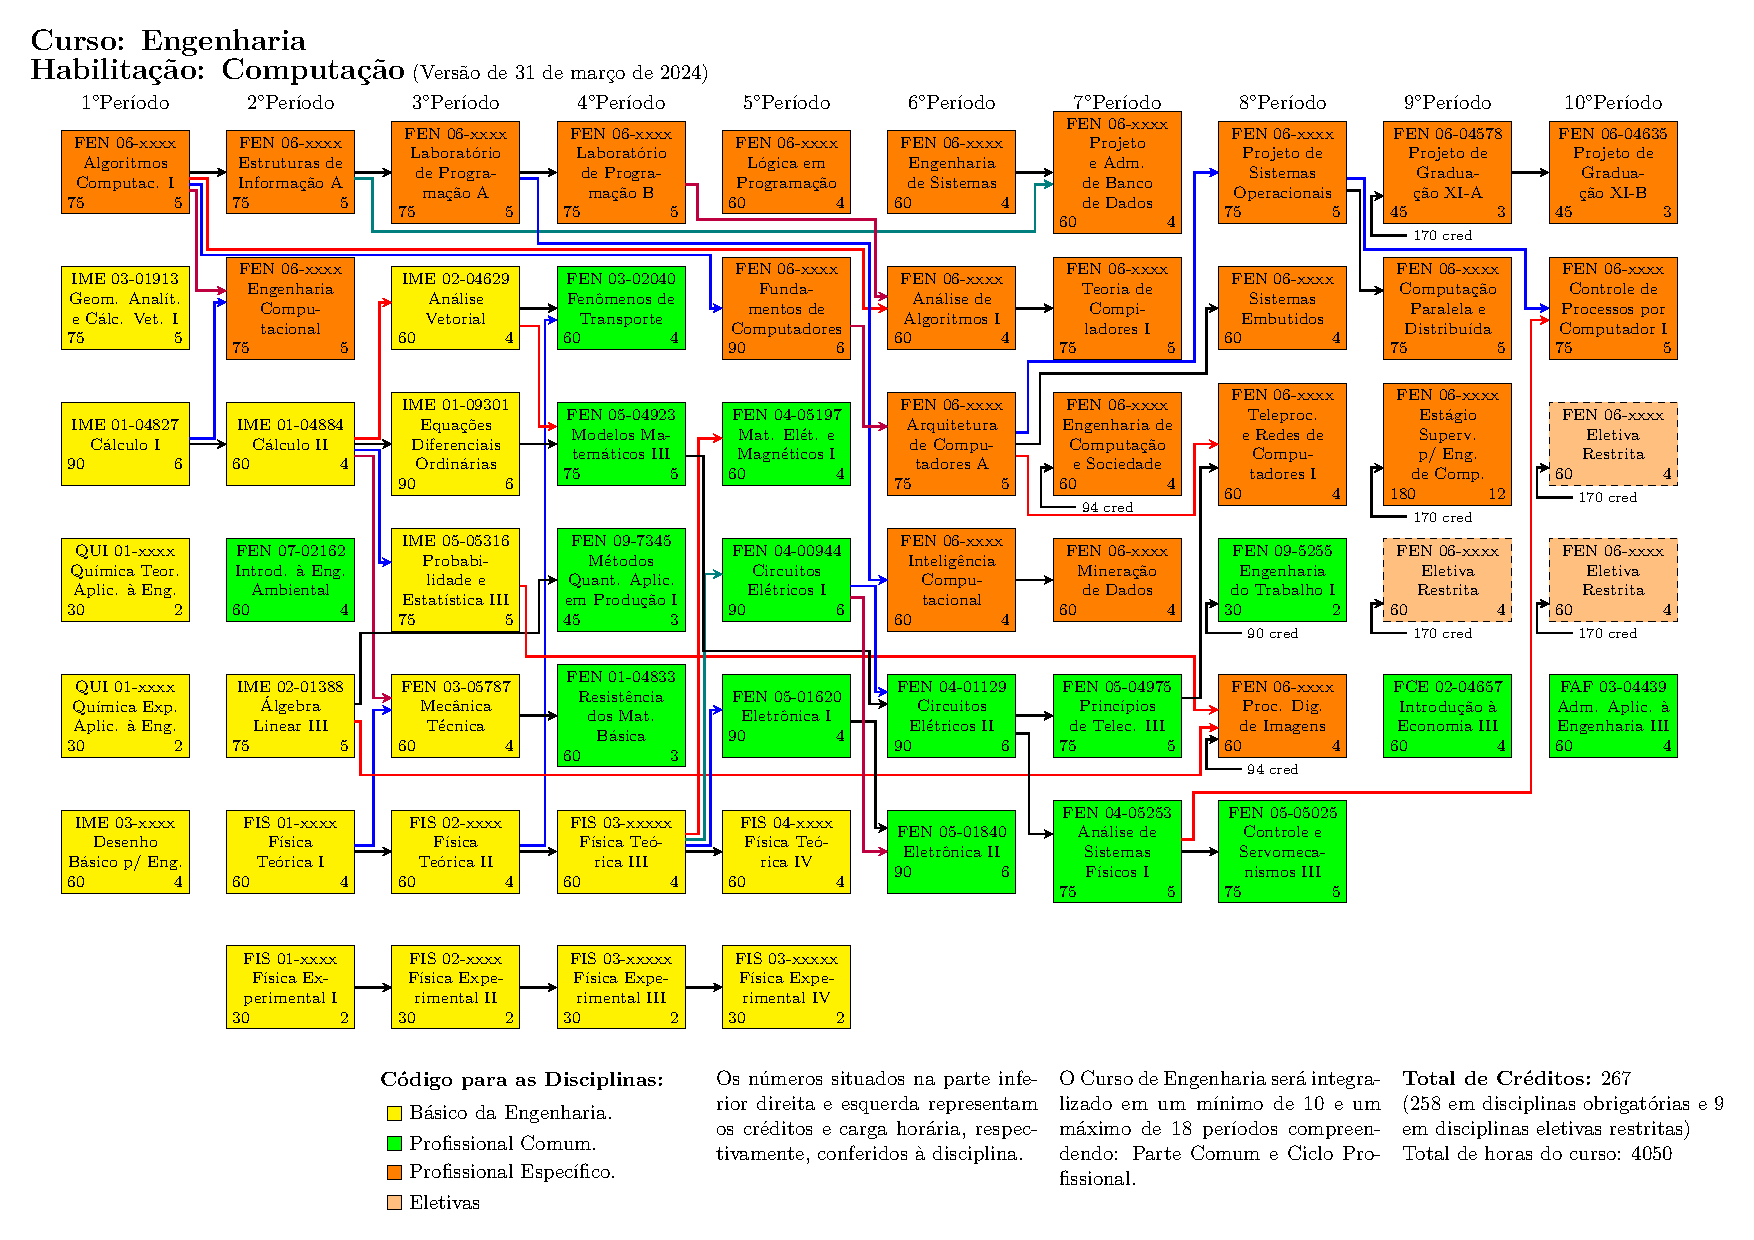
\includepdf[pages=-,angle=90]{fluxogramaEngenhariaComputacao.pdf}
\chapter{Ementas do Curso de Engenharia de Computação}
\label{ementas}
\includepdf[pages=-,addtotoc={1,section,1,{\Adm},},pagecommand={\thispagestyle{fancy}}]{ementasExternas/administracao_financeira_de_projeto.pdf}
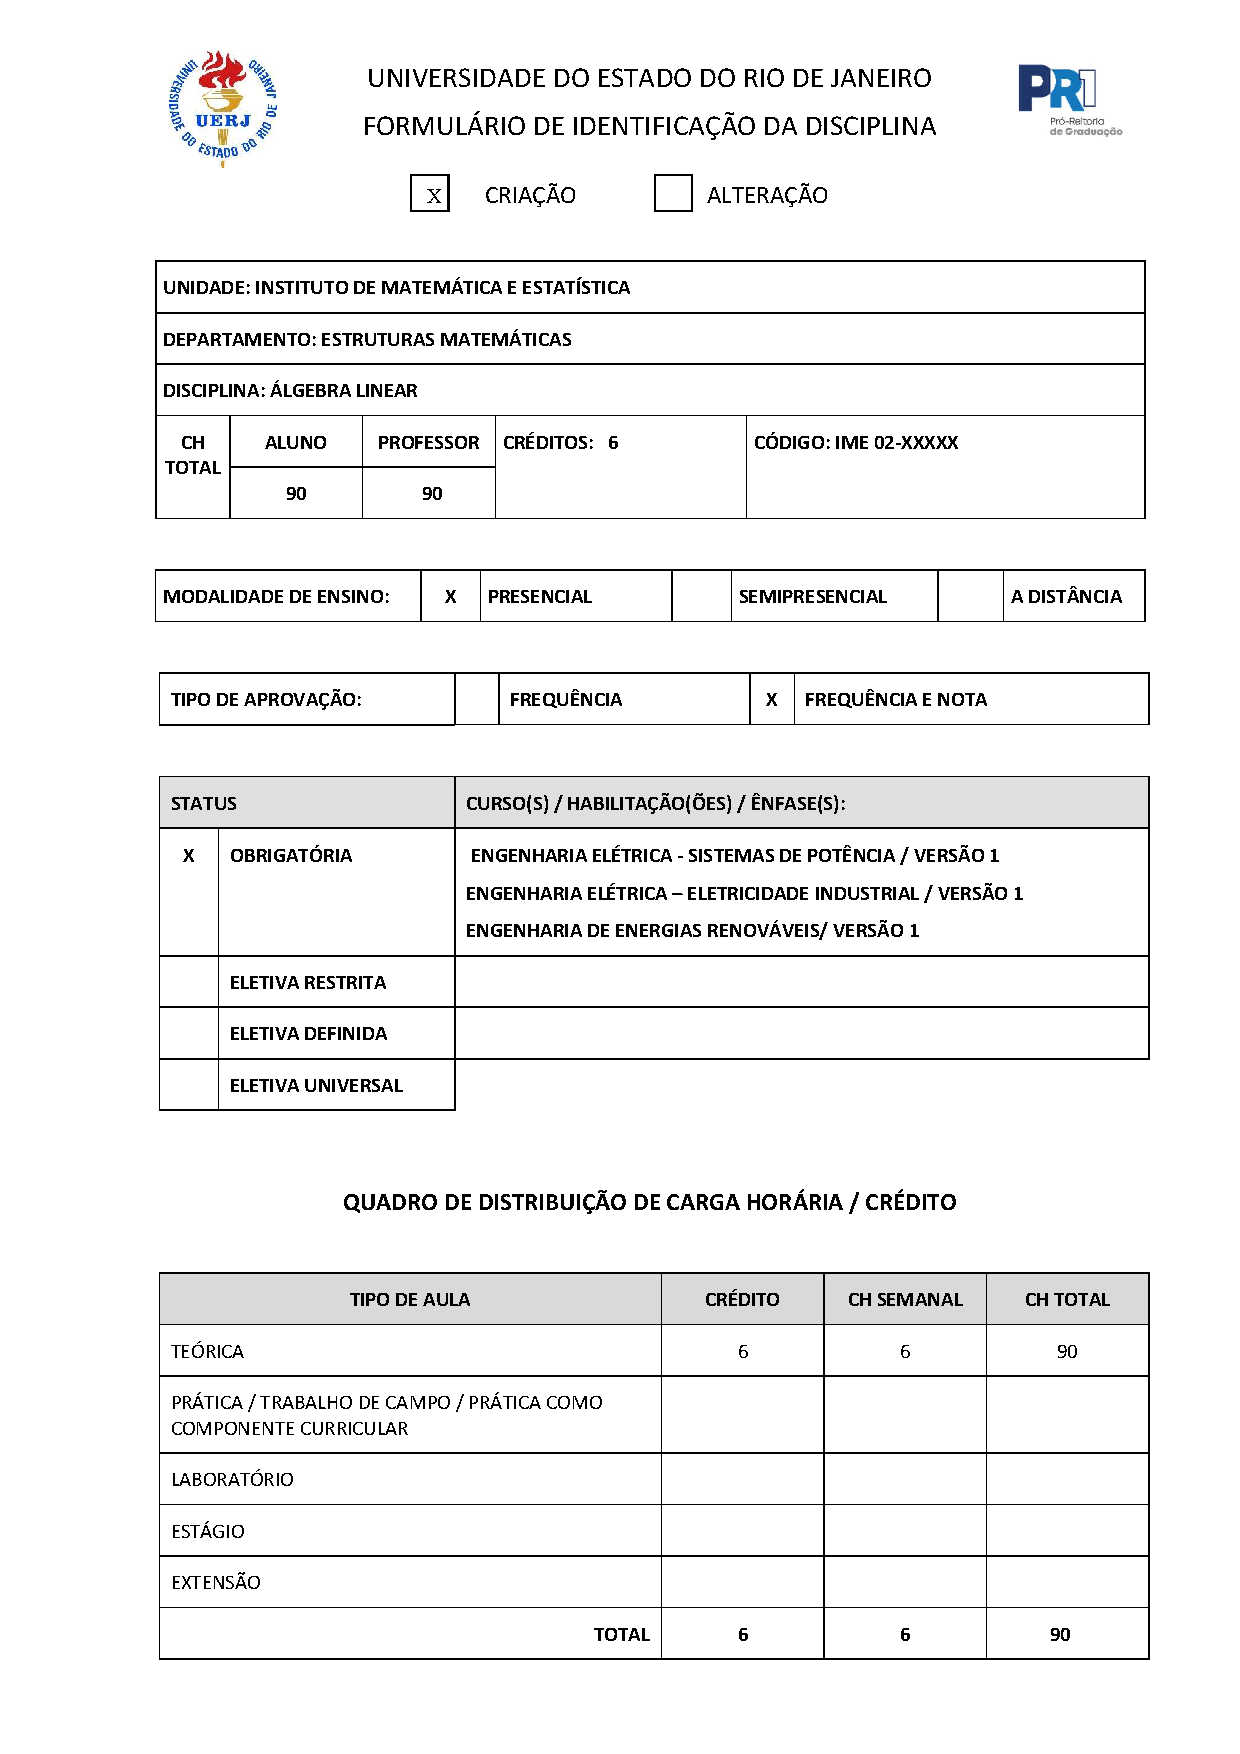
\includepdf[pages=-,addtotoc={1,section,1,{\AlgLin},},pagecommand={\thispagestyle{fancy}}]{ementasExternas/Algebra_Linear_90hs.pdf}
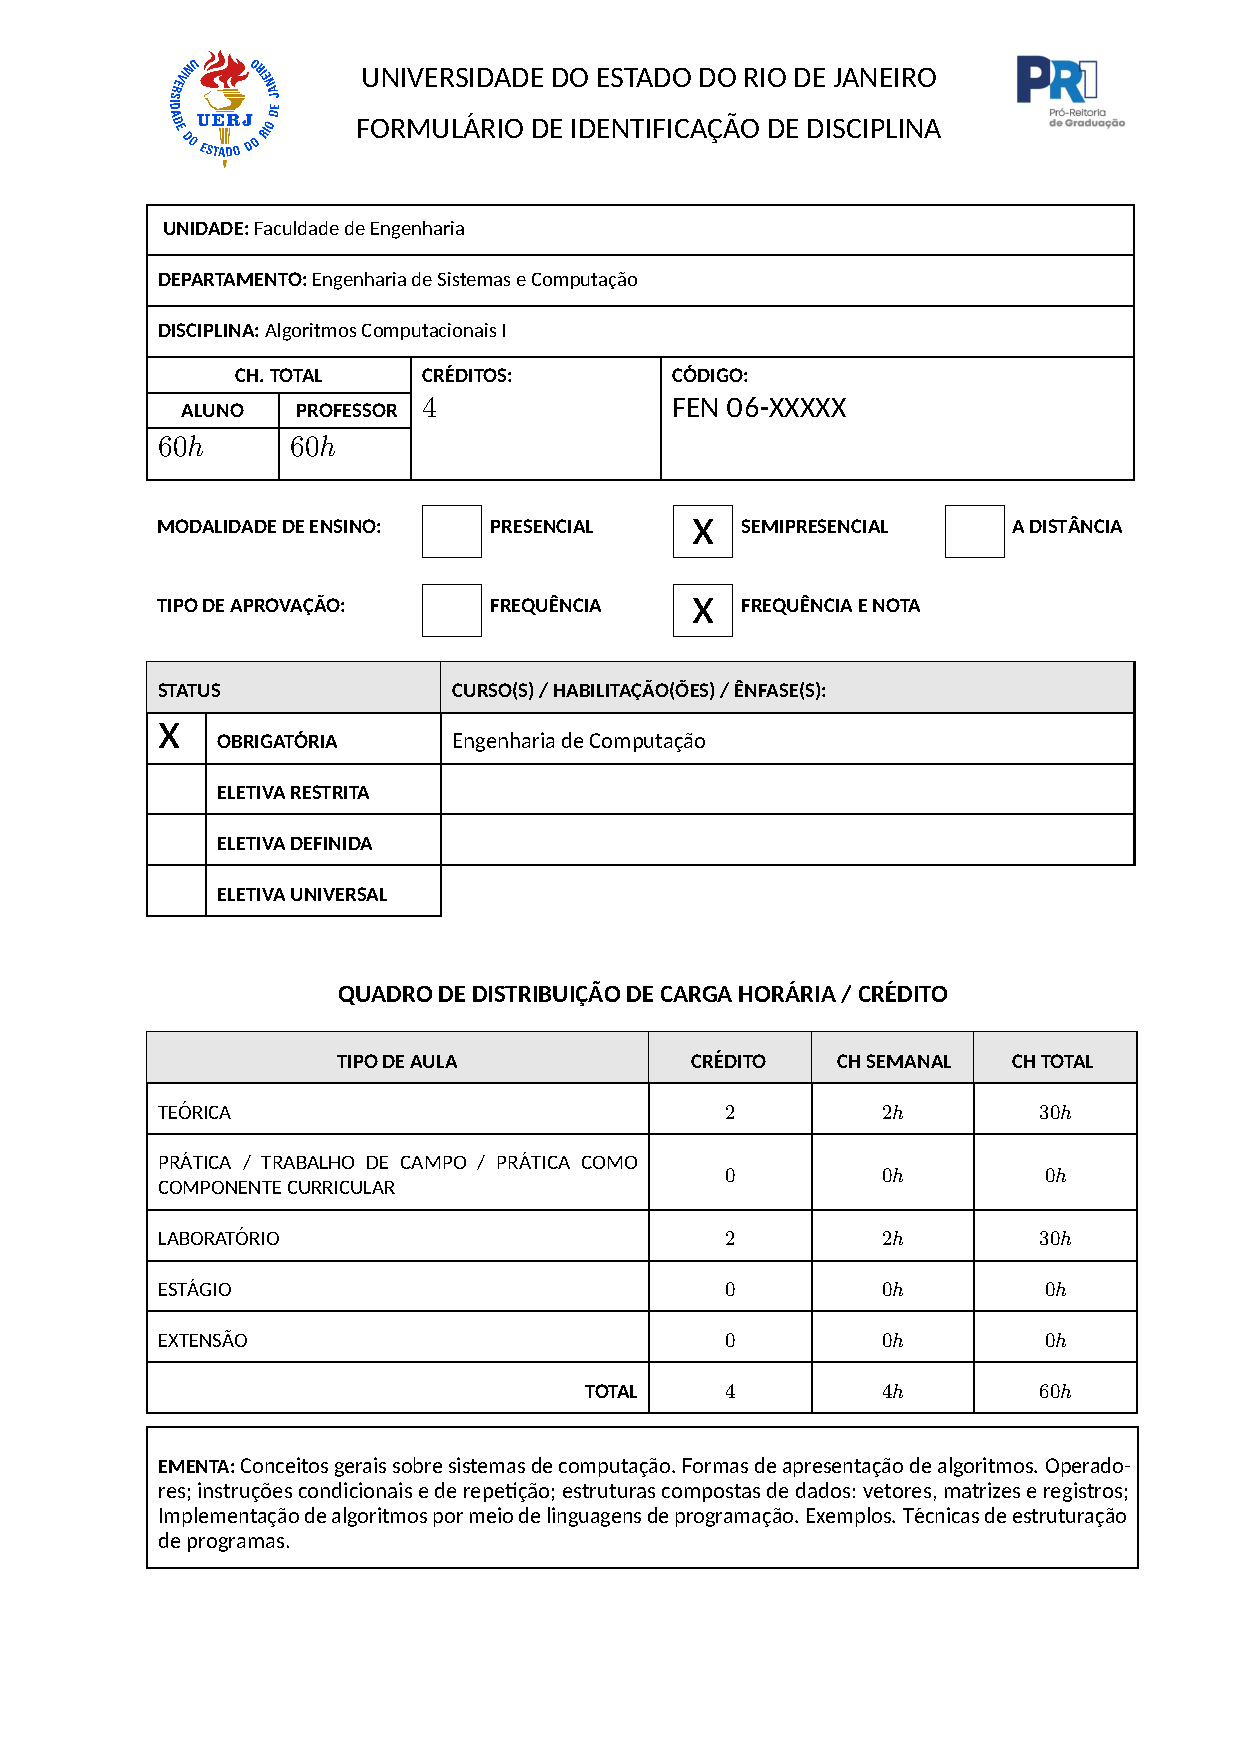
\includepdf[pages=-,addtotoc={1,section,1,{\AlgComp},},pagecommand={\thispagestyle{fancy}}]{ementas/AlgoritmosComputacionais.pdf}
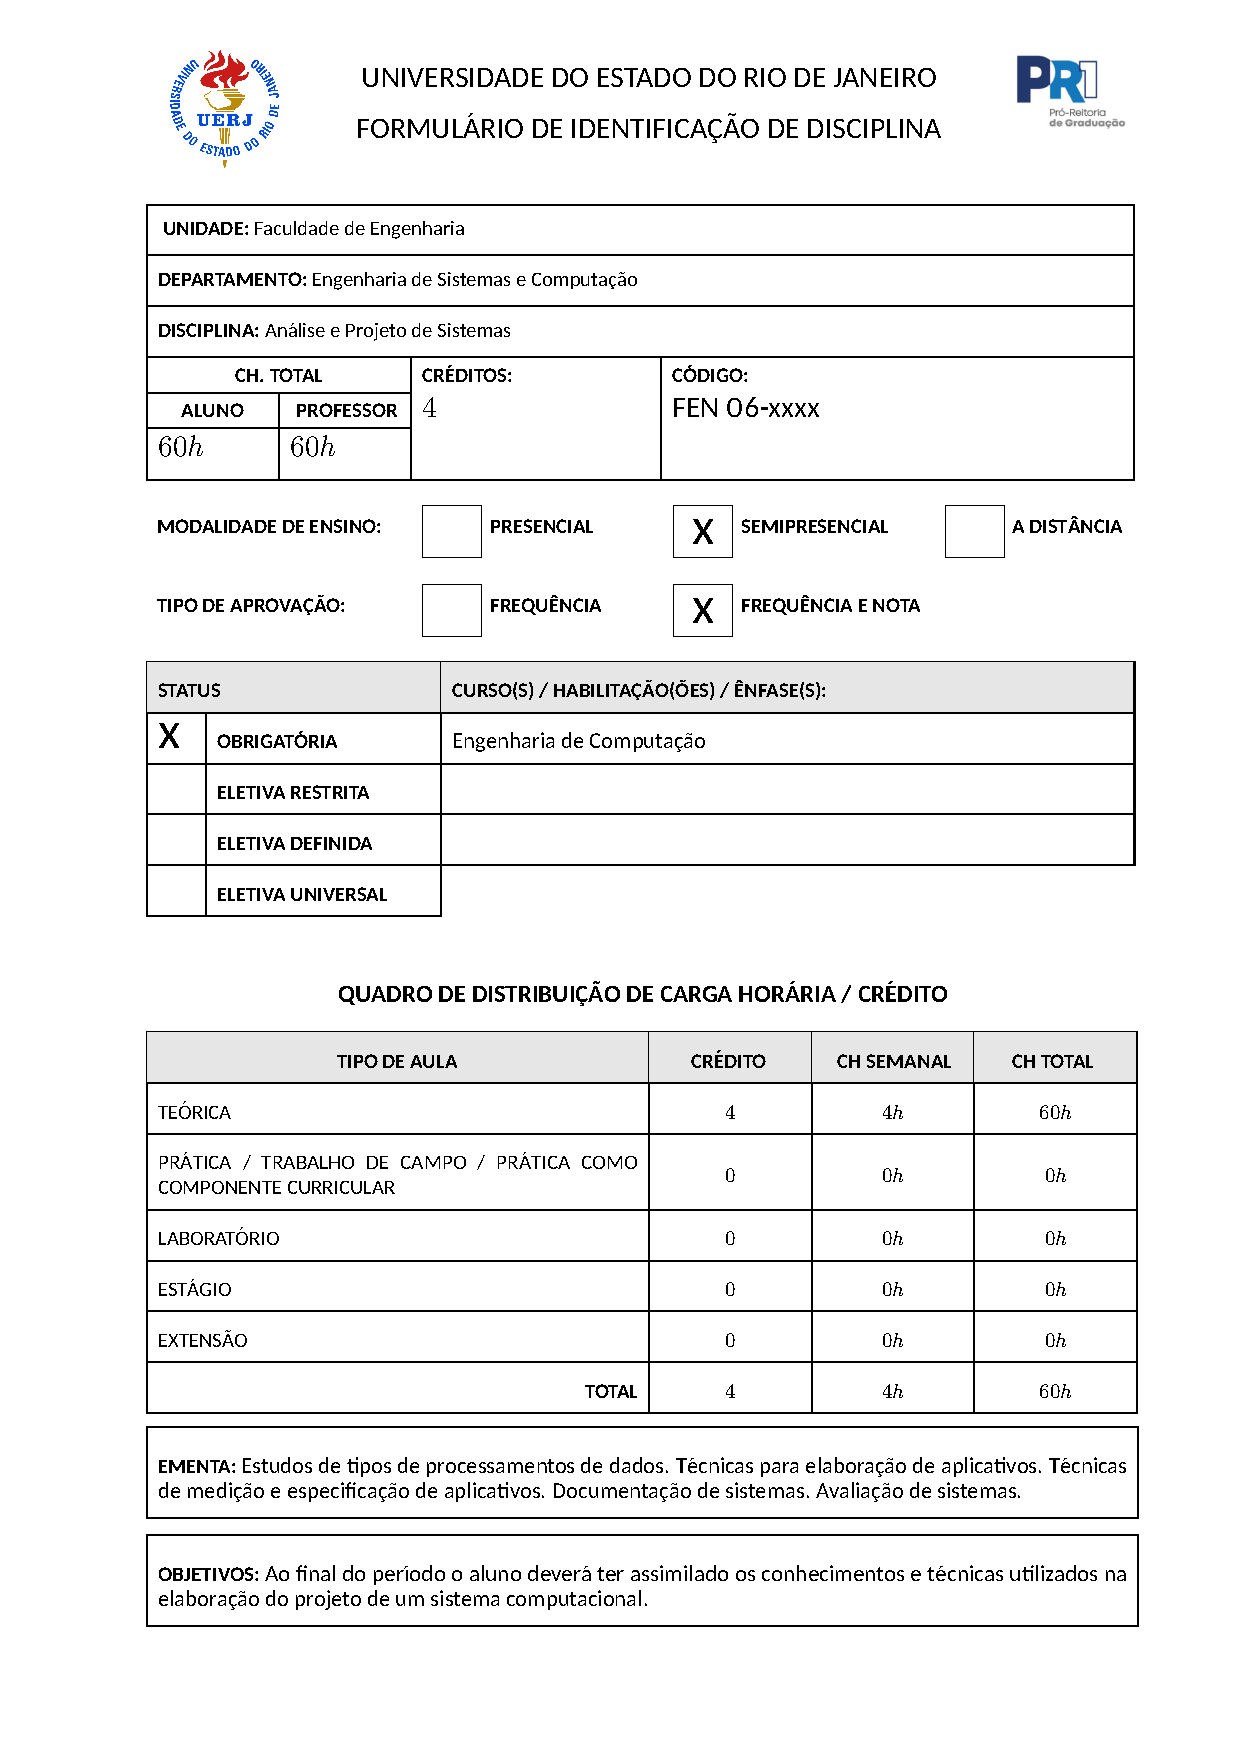
\includepdf[pages=-,addtotoc={1,section,1,{\AnaProjSist},},pagecommand={\thispagestyle{fancy}}]{ementas/analise_e_projeto_de_sistemas.pdf}
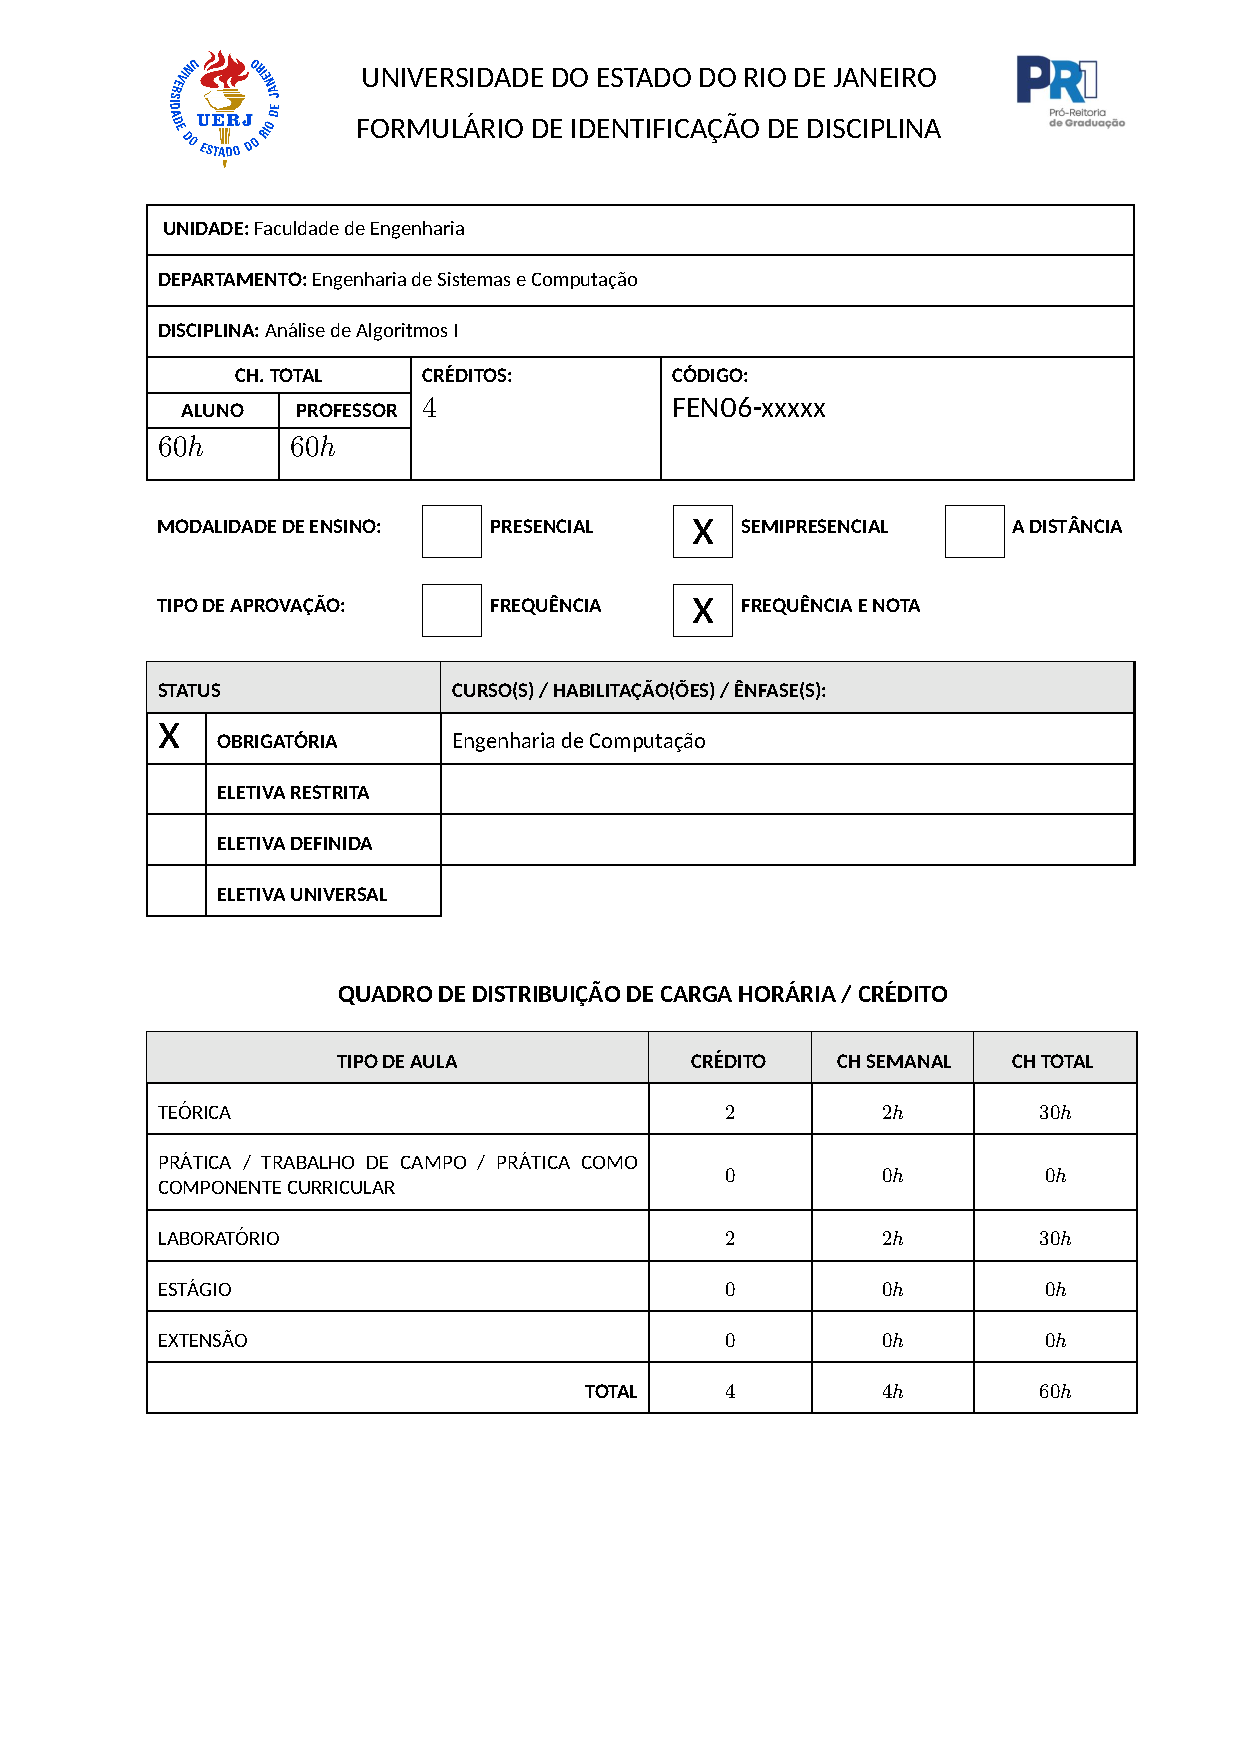
\includepdf[pages=-,addtotoc={1,section,1,{\AnAlg},},pagecommand={\thispagestyle{fancy}}]{ementas/AnaliseDeAlgoritmos.pdf}
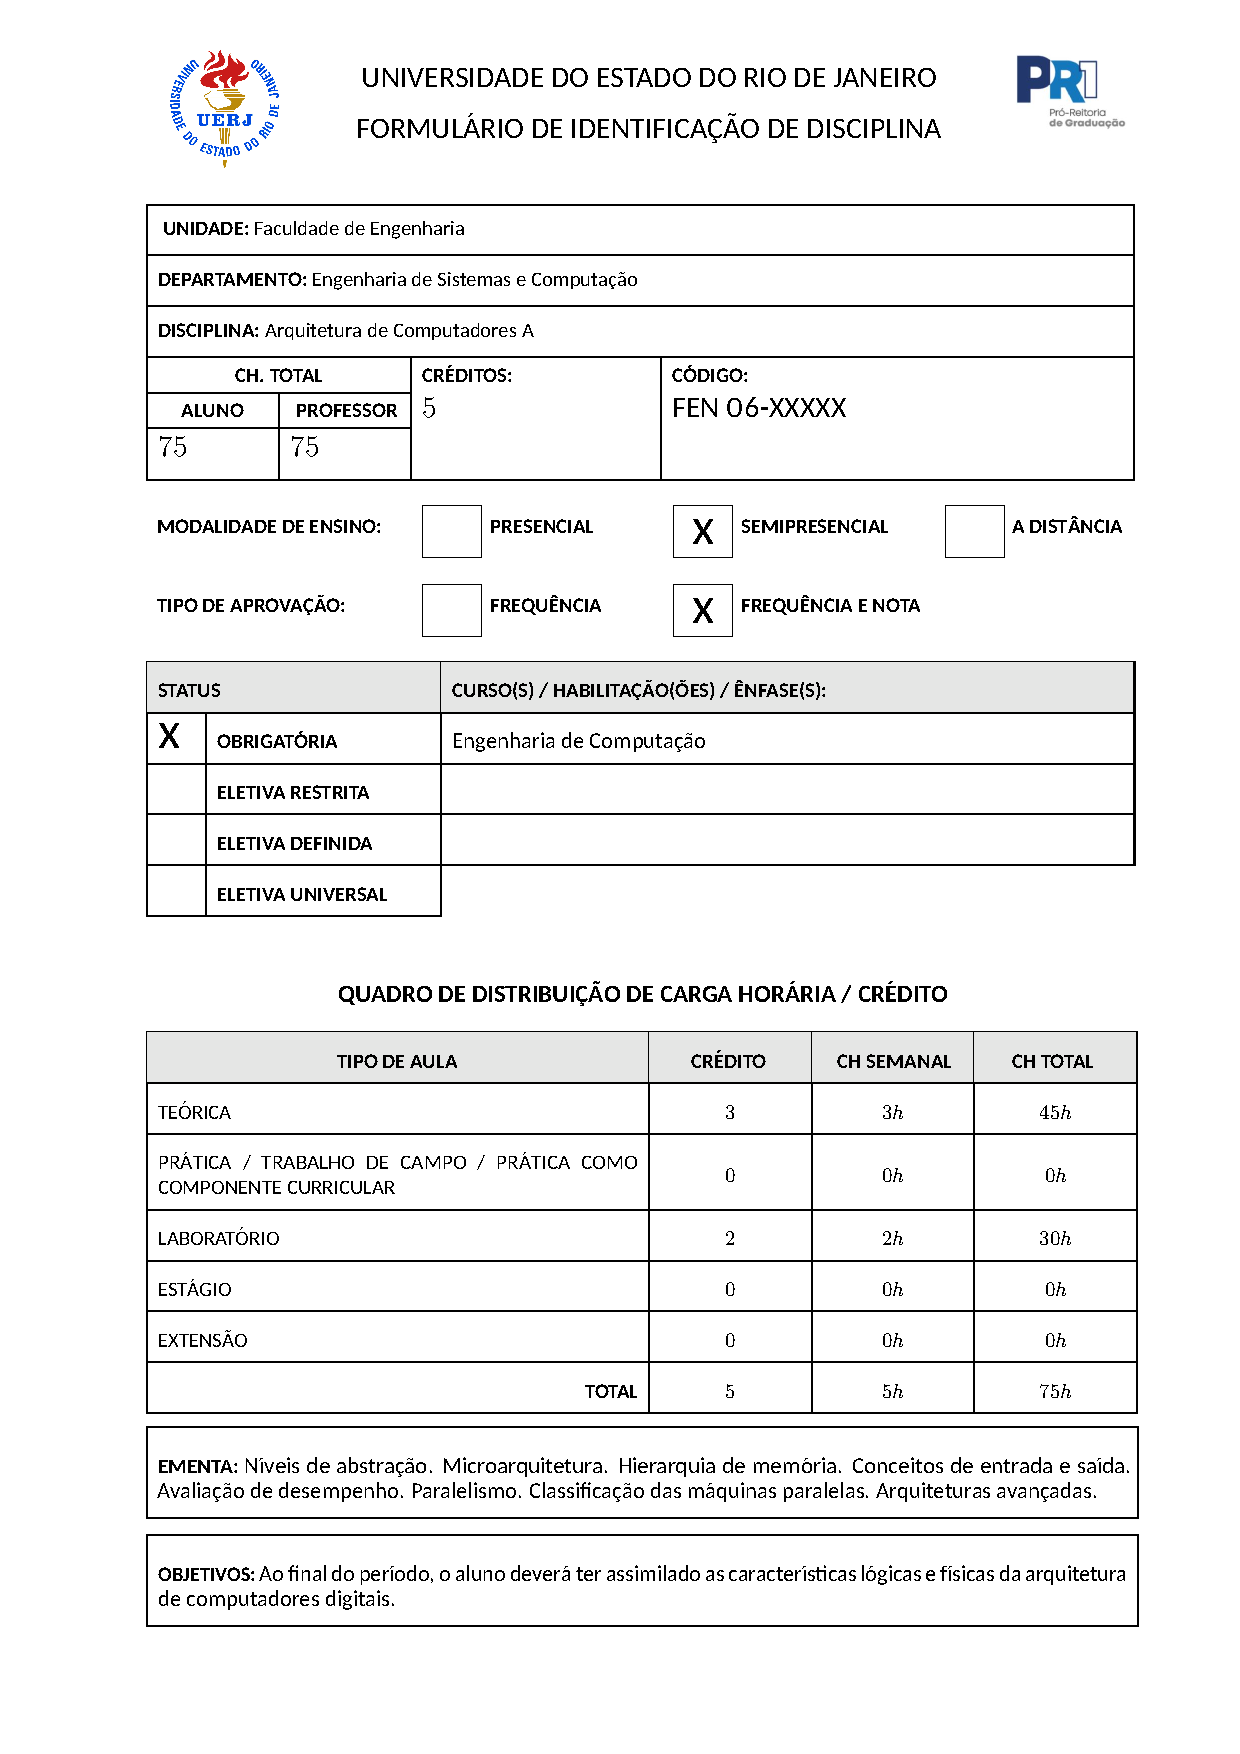
\includepdf[pages=-,addtotoc={1,section,1,{\ArqComp},},pagecommand={\thispagestyle{fancy}}]{ementas/ArquiteturaDeComputadores.pdf}
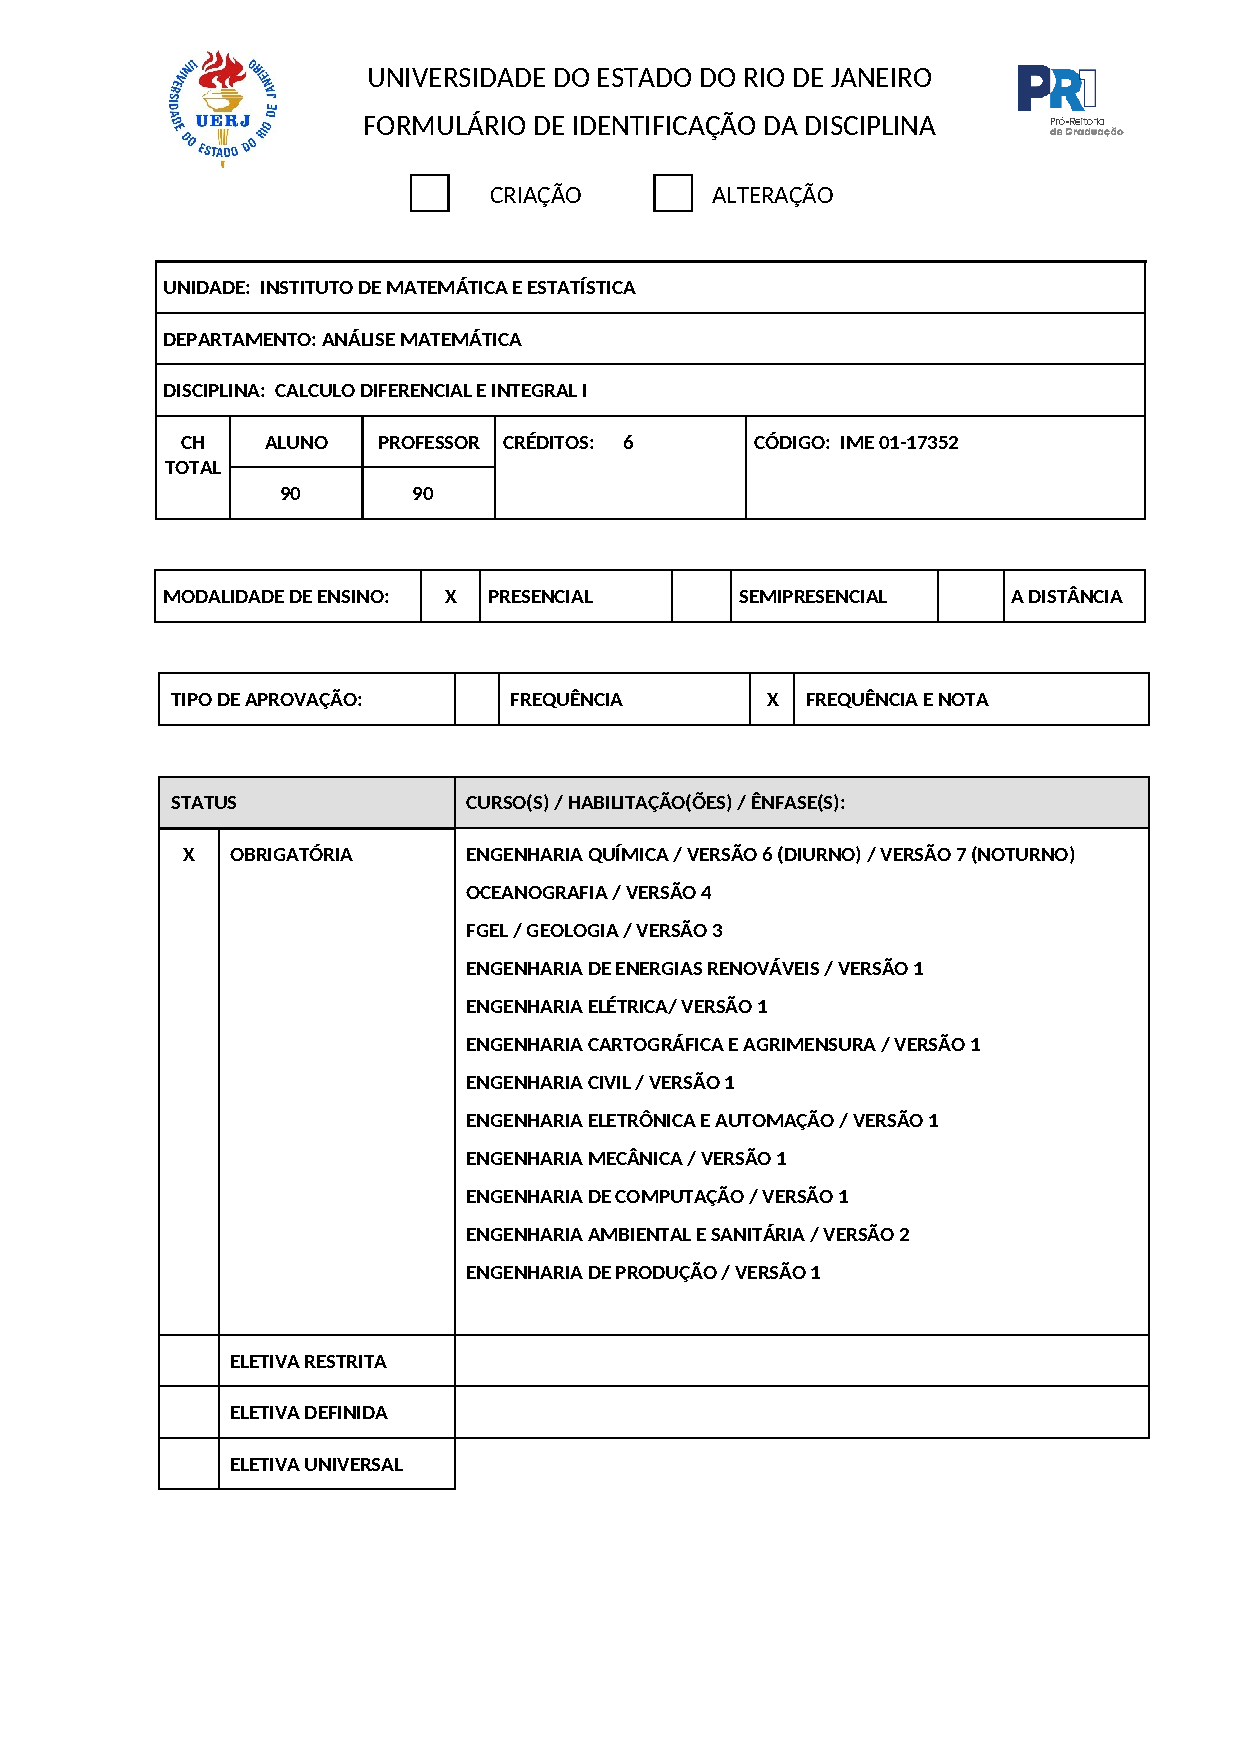
\includepdf[pages=-,addtotoc={1,section,1,{\CalcI},},pagecommand={\thispagestyle{fancy}}]{ementasExternas/calculo_diferencial_e_integral_i.pdf}
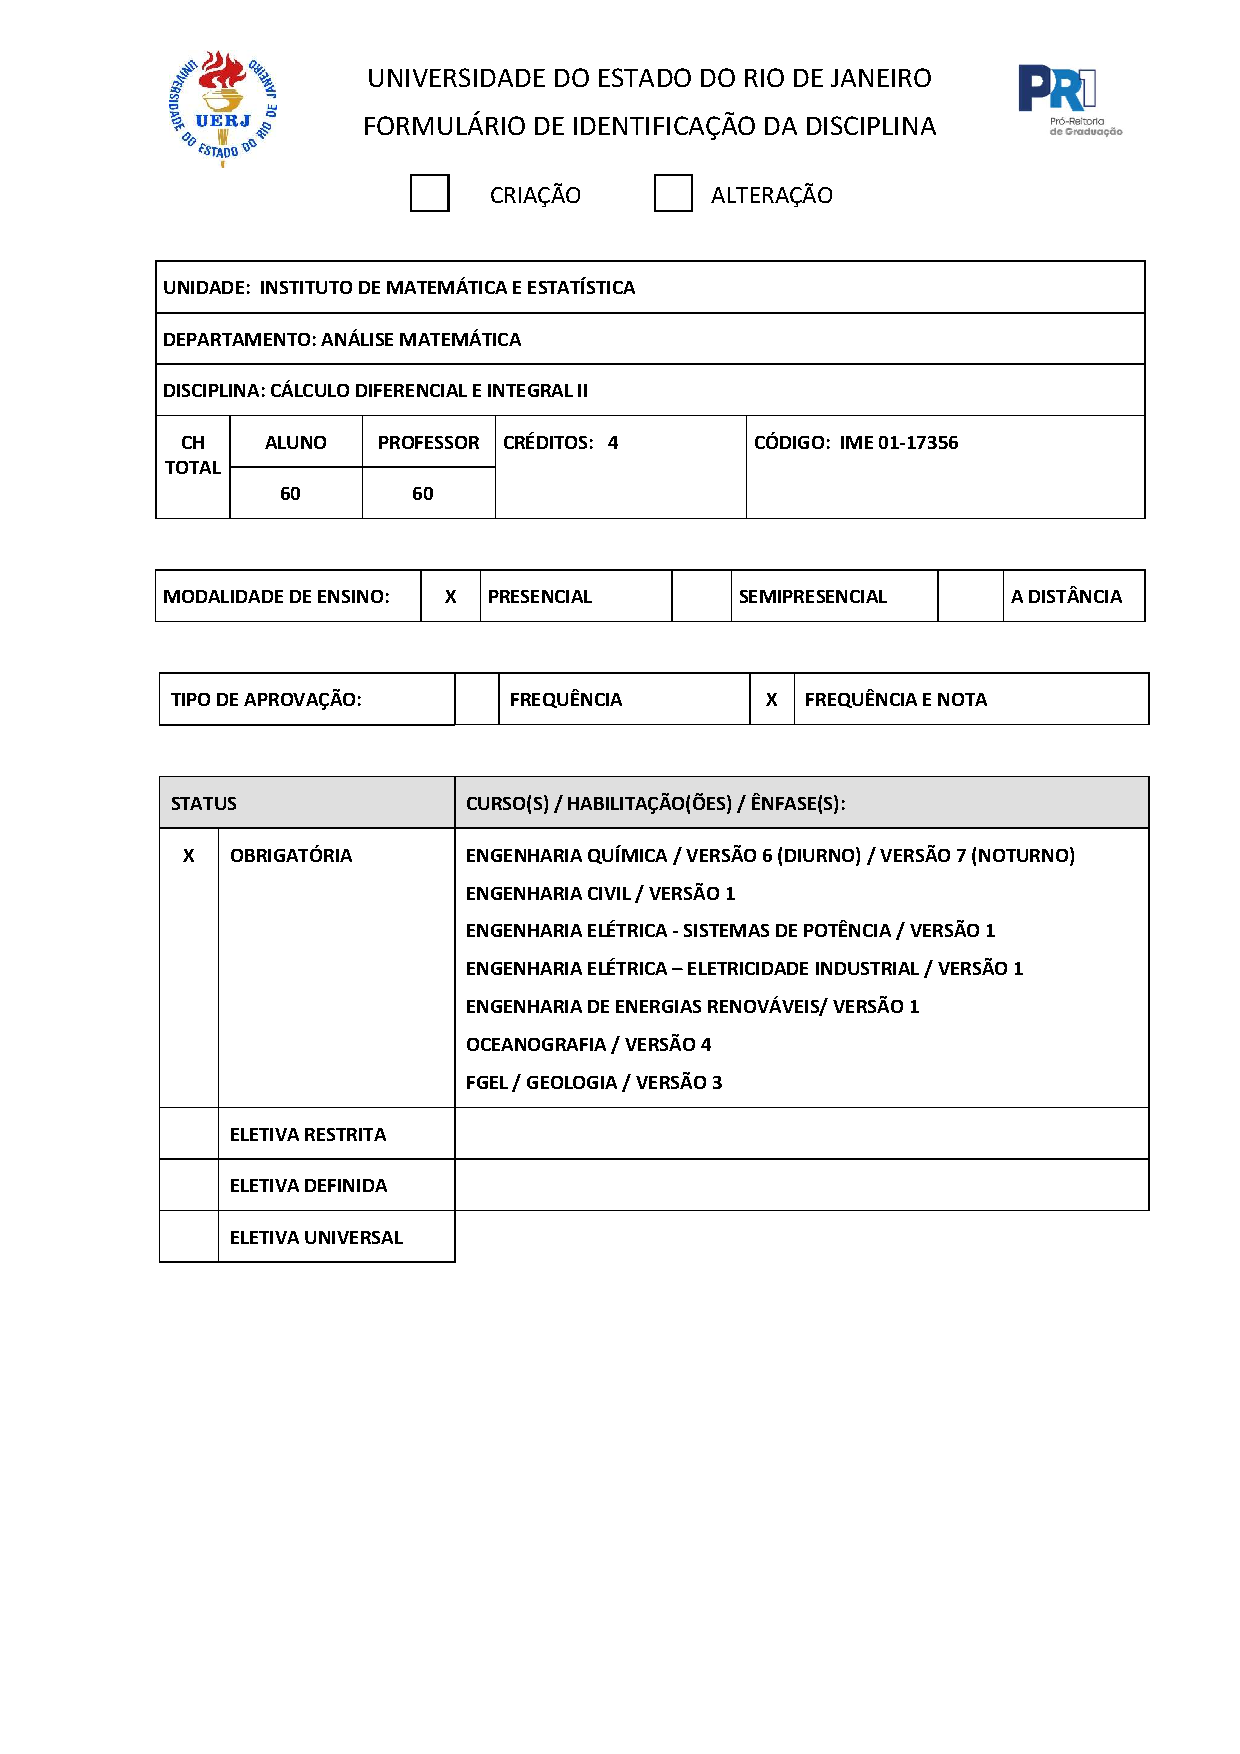
\includepdf[pages=-,addtotoc={1,section,1,{\CalcII},},pagecommand={\thispagestyle{fancy}}]{ementasExternas/calculo_diferencial_e_integral_ii.pdf}
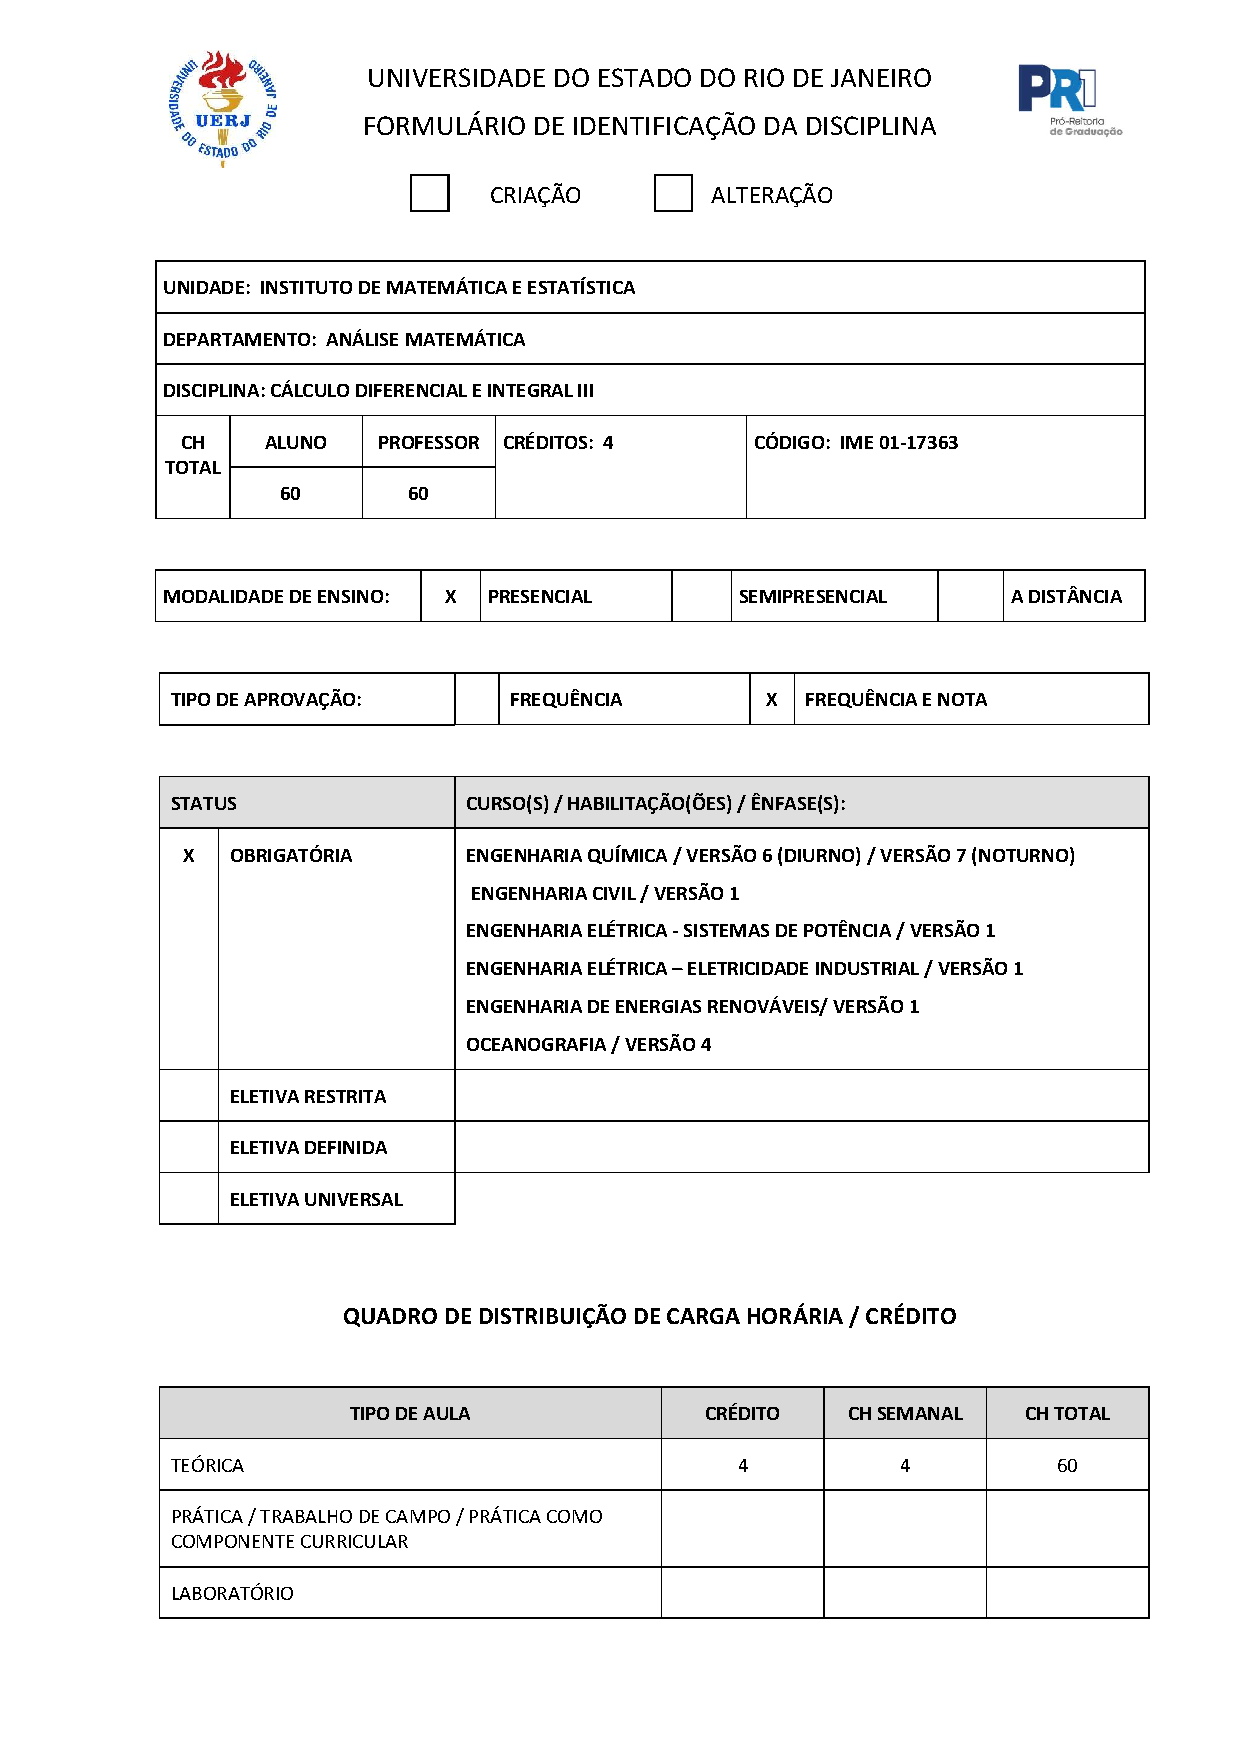
\includepdf[pages=-,addtotoc={1,section,1,{\CalcIII},},pagecommand={\thispagestyle{fancy}}]{ementasExternas/calculo_diferencial_e_integral_iii.pdf}
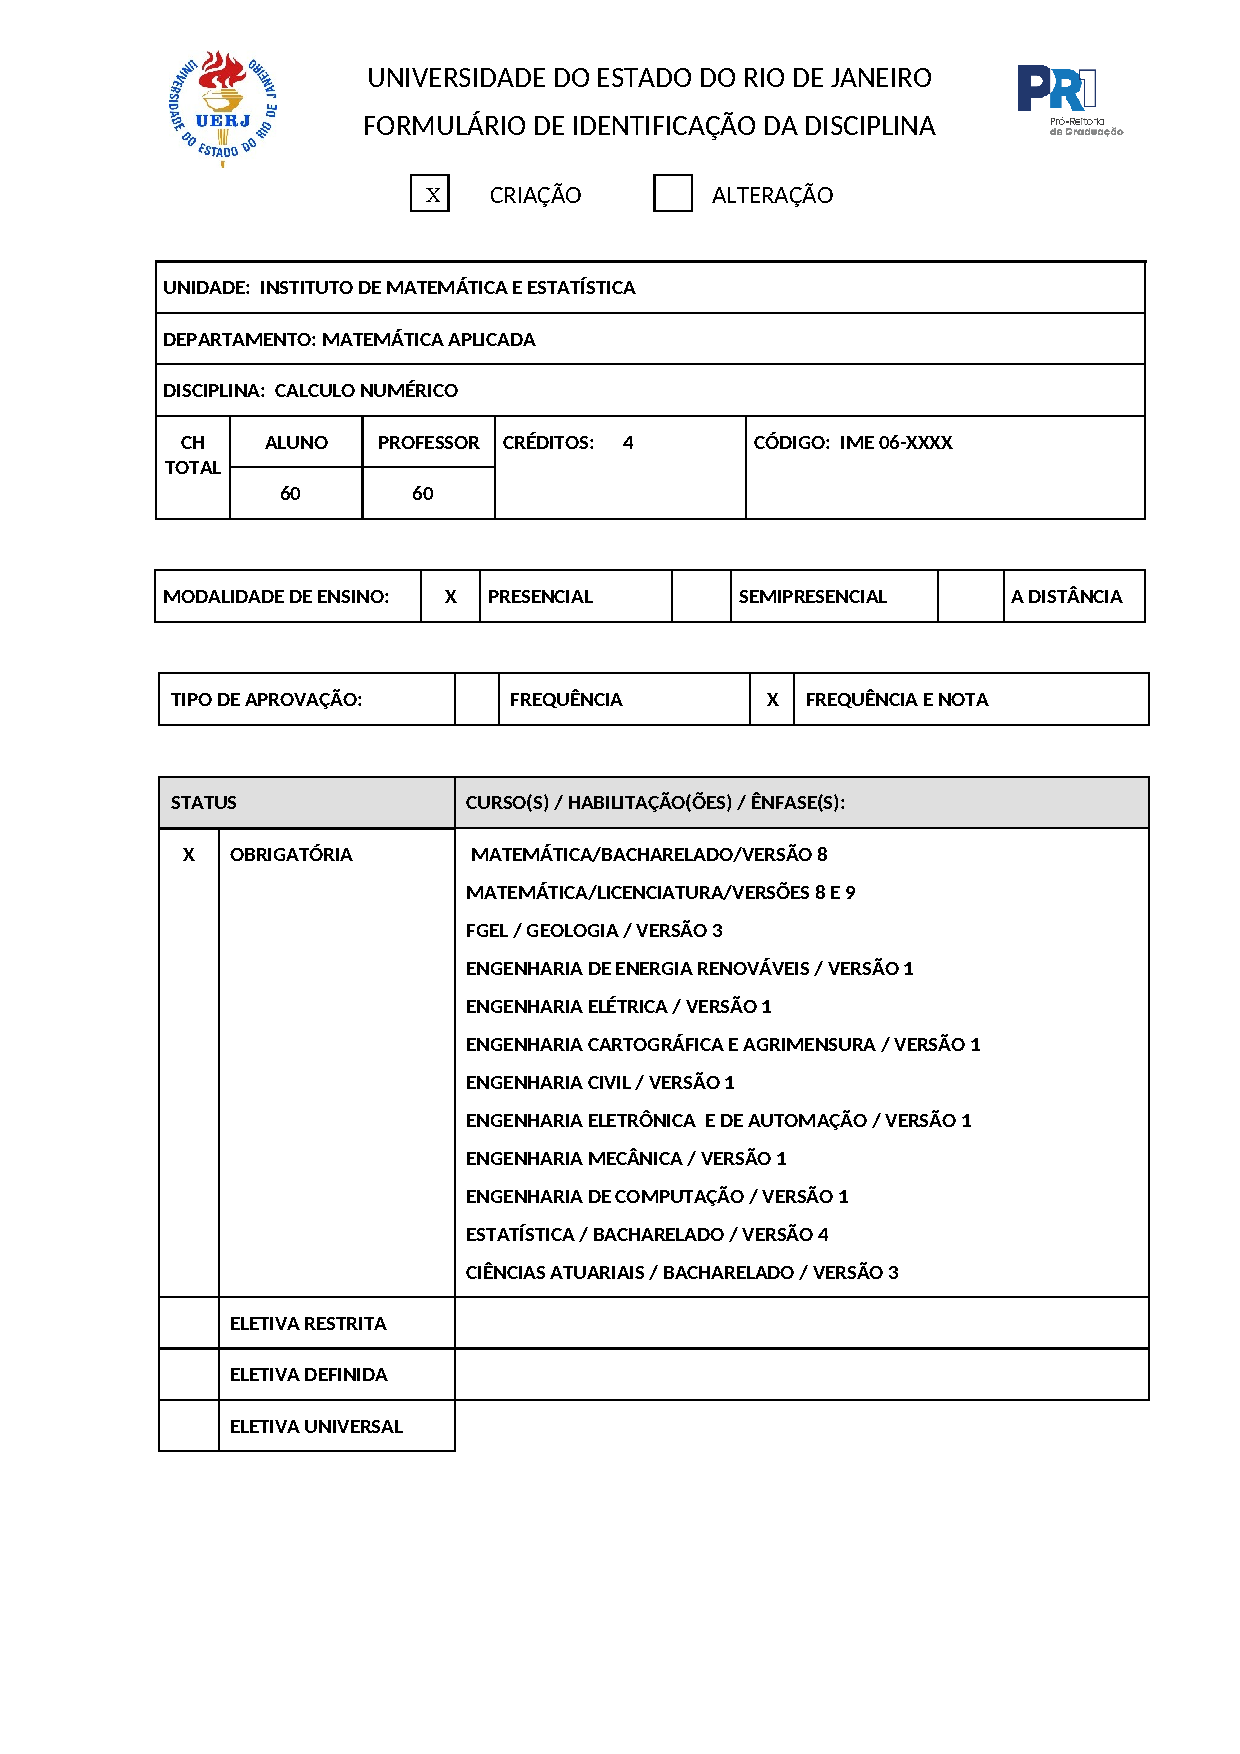
\includepdf[pages=-,addtotoc={1,section,1,{\CalcNum},},pagecommand={\thispagestyle{fancy}}]{ementasExternas/Calculo_Numerico.pdf}
\includepdf[pages=-,addtotoc={1,section,1,{\CalcNum},},pagecommand={\thispagestyle{fancy}}]{ementasExternas/circuitos_eletronicos_i.pdf}% Circuitos Eletrônicos I
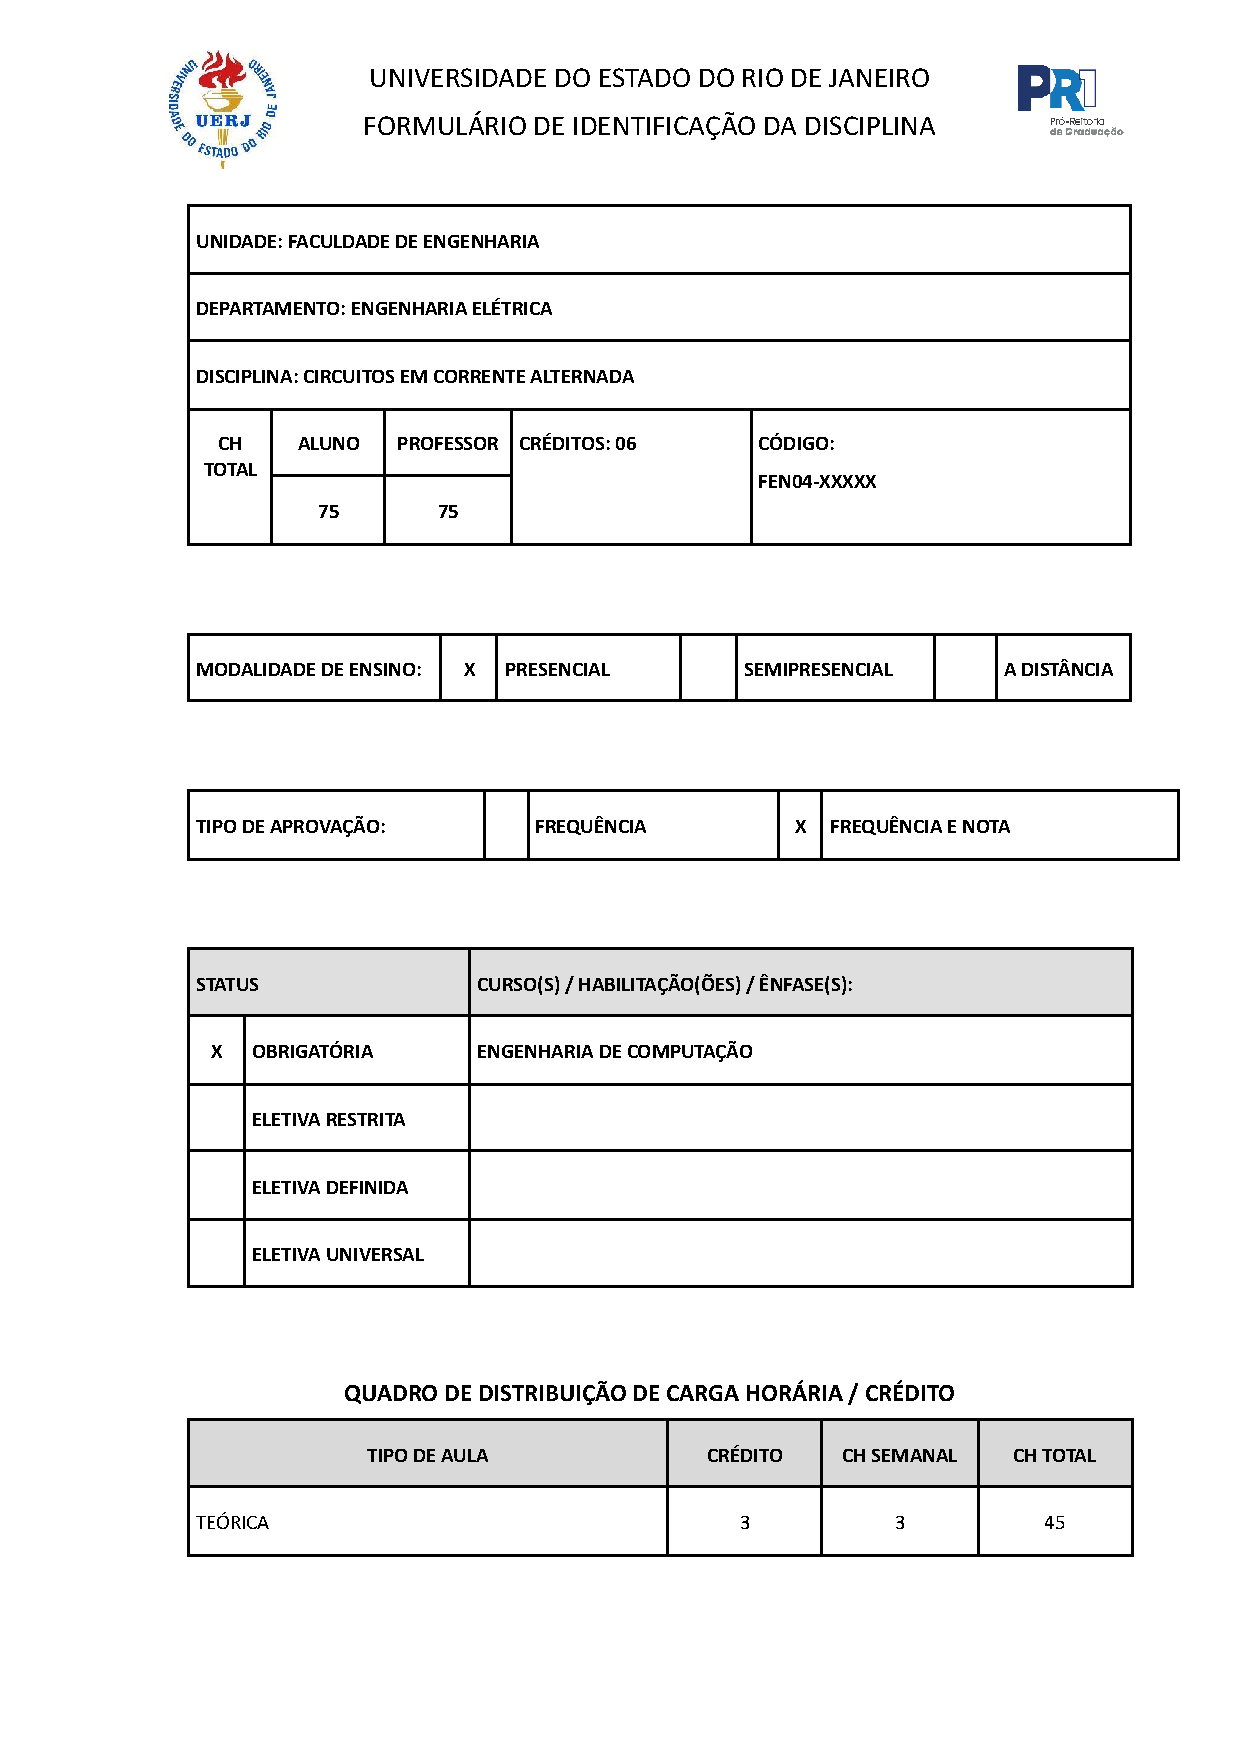
\includepdf[pages=-,addtotoc={1,section,1,{\CCA},},pagecommand={\thispagestyle{fancy}}]{ementasExternas/Eletrica/CircuitosemCorrenteAlternada.pdf}
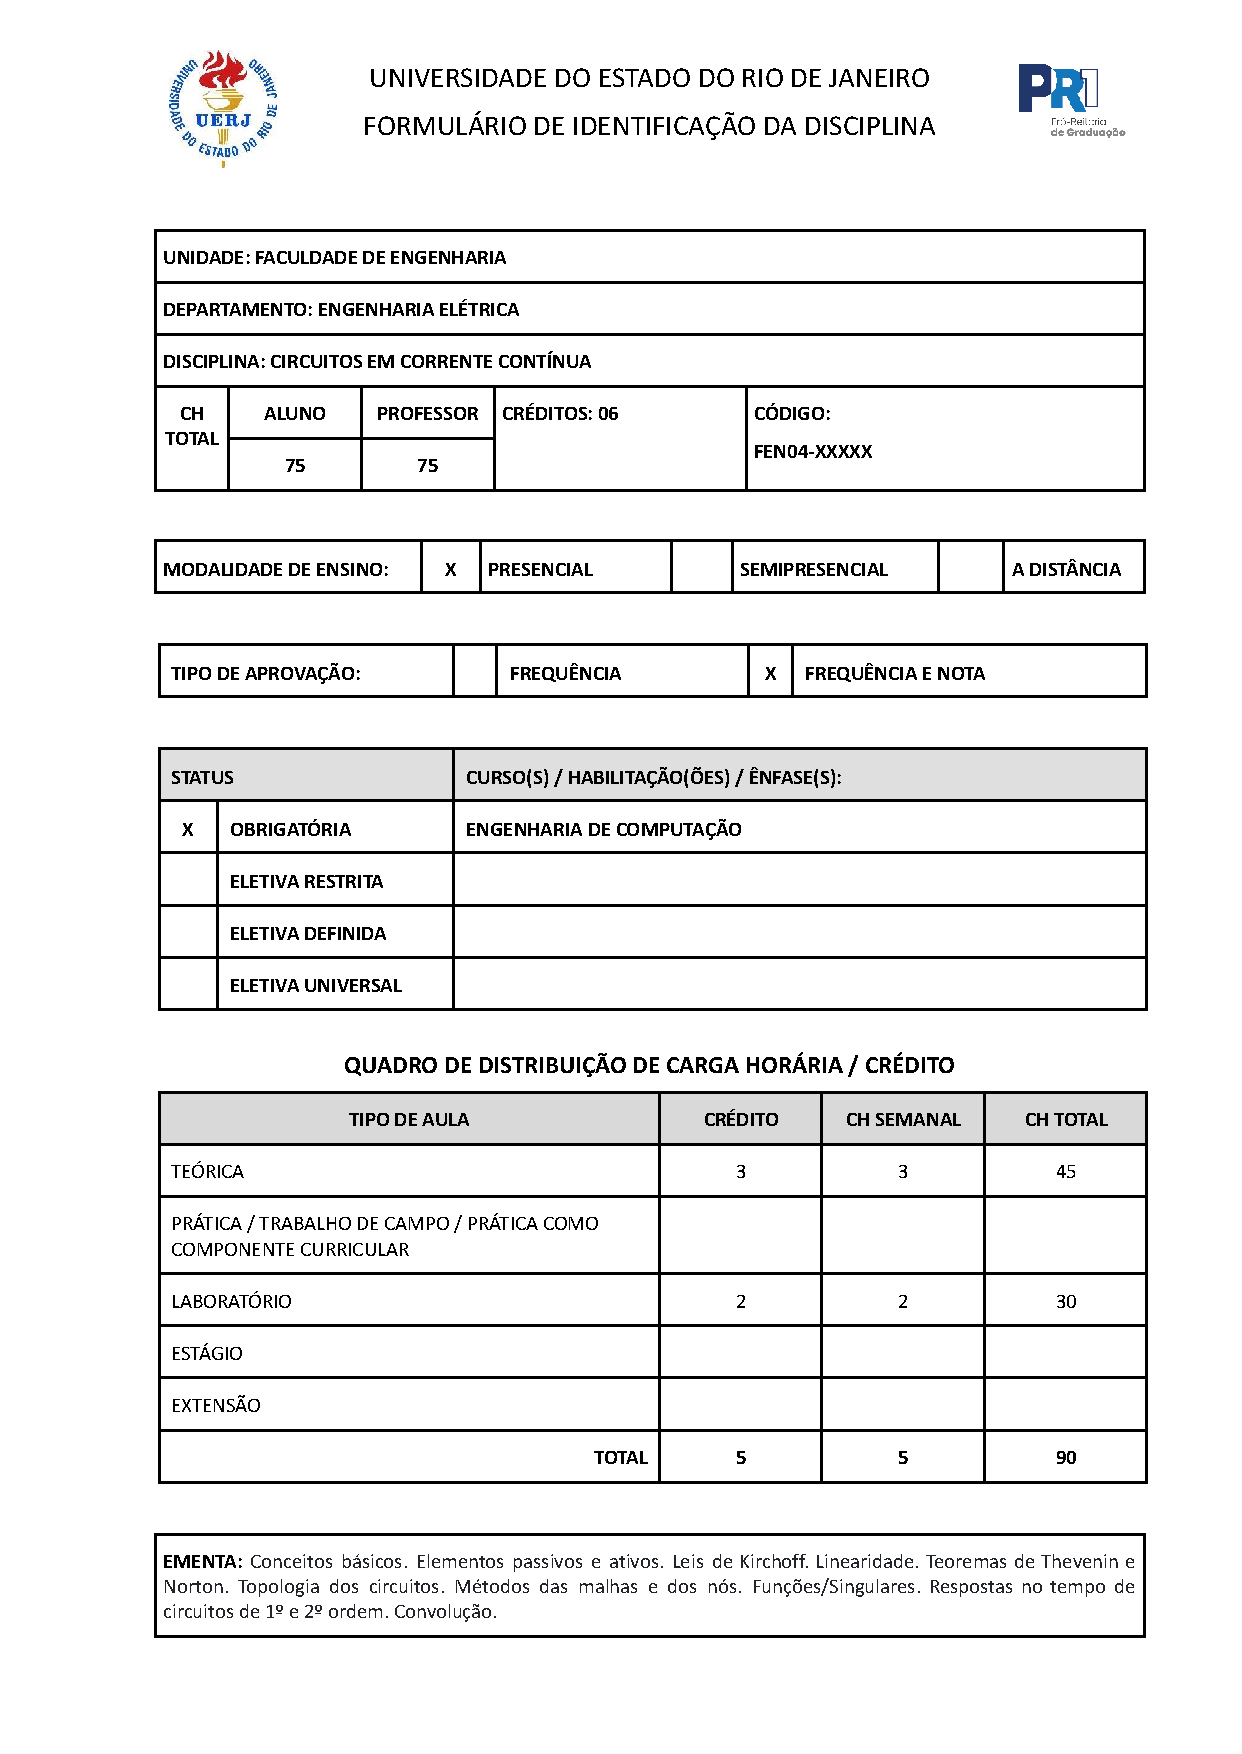
\includepdf[pages=-,addtotoc={1,section,1,{\CCC},},pagecommand={\thispagestyle{fancy}}]{ementasExternas/Eletrica/CircuitosemCorrenteContinua.pdf}
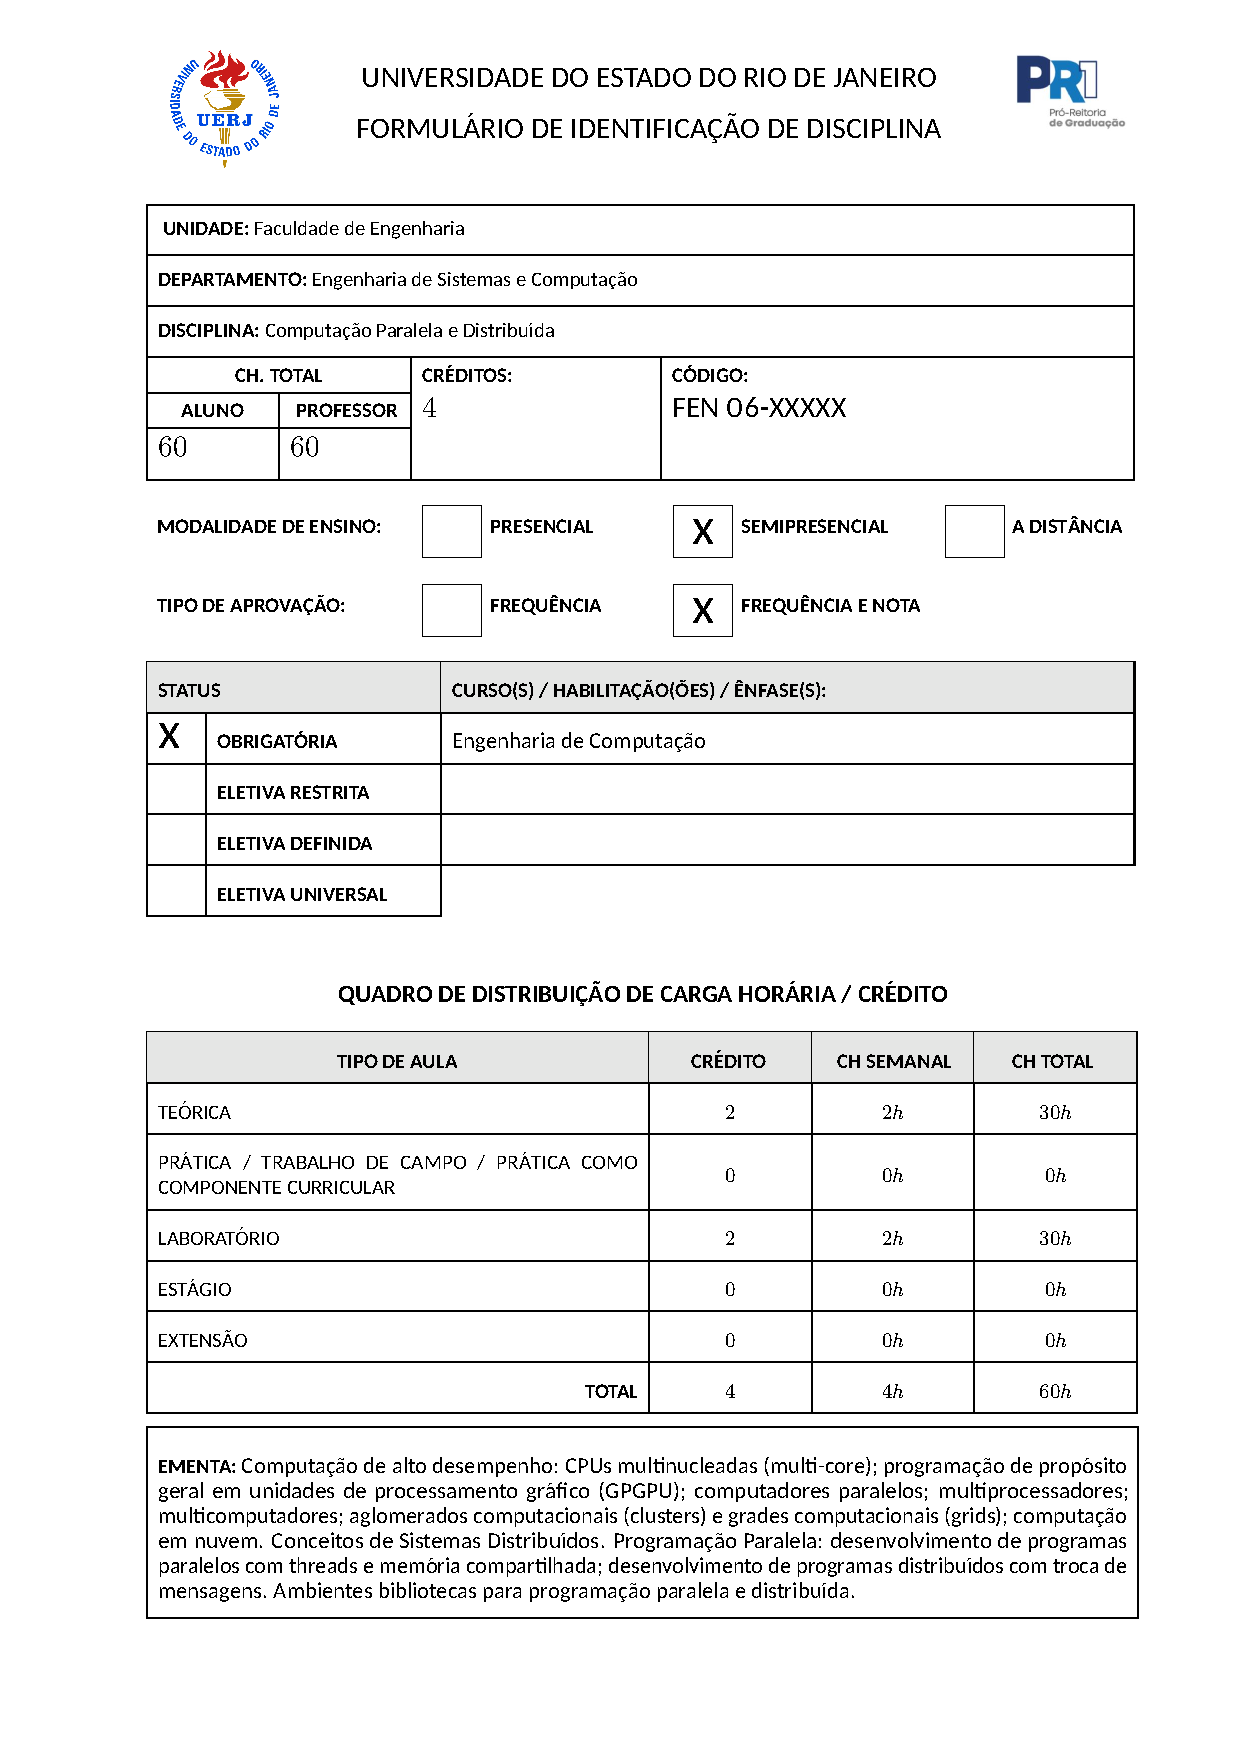
\includepdf[pages=-,addtotoc={1,section,1,{\CompParal},},pagecommand={\thispagestyle{fancy}}]{ementas/ComputacaoParalela.pdf}
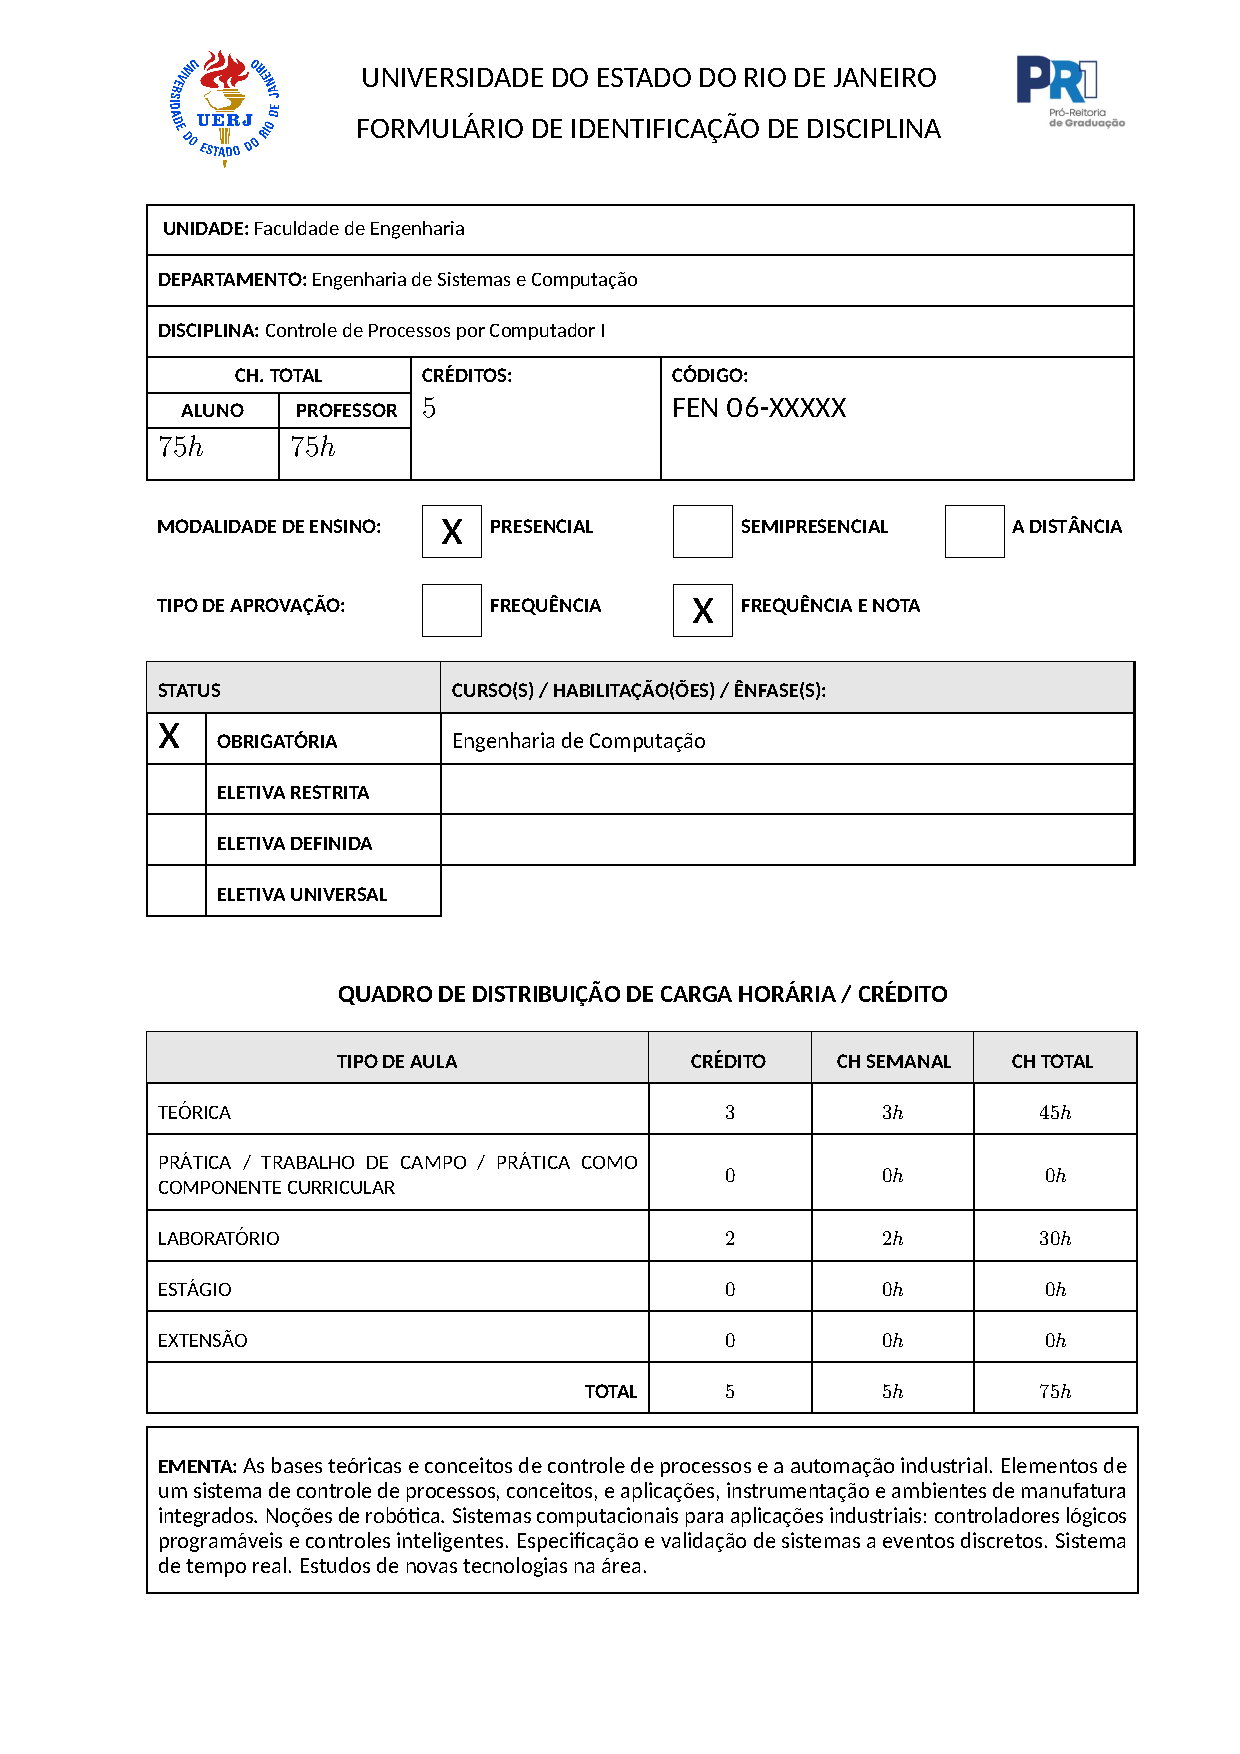
\includepdf[pages=-,addtotoc={1,section,1,{\Control},},pagecommand={\thispagestyle{fancy}}]{ementas/ControleDeProcessosPorComputador.pdf}
\includepdf[pages=-,addtotoc={1,section,1,{\FisIII},},pagecommand={\thispagestyle{fancy}}]{ementasExternas/eletromagnetismo_basico_experimental.pdf}
\includepdf[pages=-,addtotoc={1,section,1,{\FisEIII},},pagecommand={\thispagestyle{fancy}}]{ementasExternas/eletromagnetismo_basico_teorico.pdf}
\includepdf[pages=-,addtotoc={1,section,1,{\Empre},},pagecommand={\thispagestyle{fancy}}]{ementasExternas/empreendedorismo_na_engenharia.pdf}
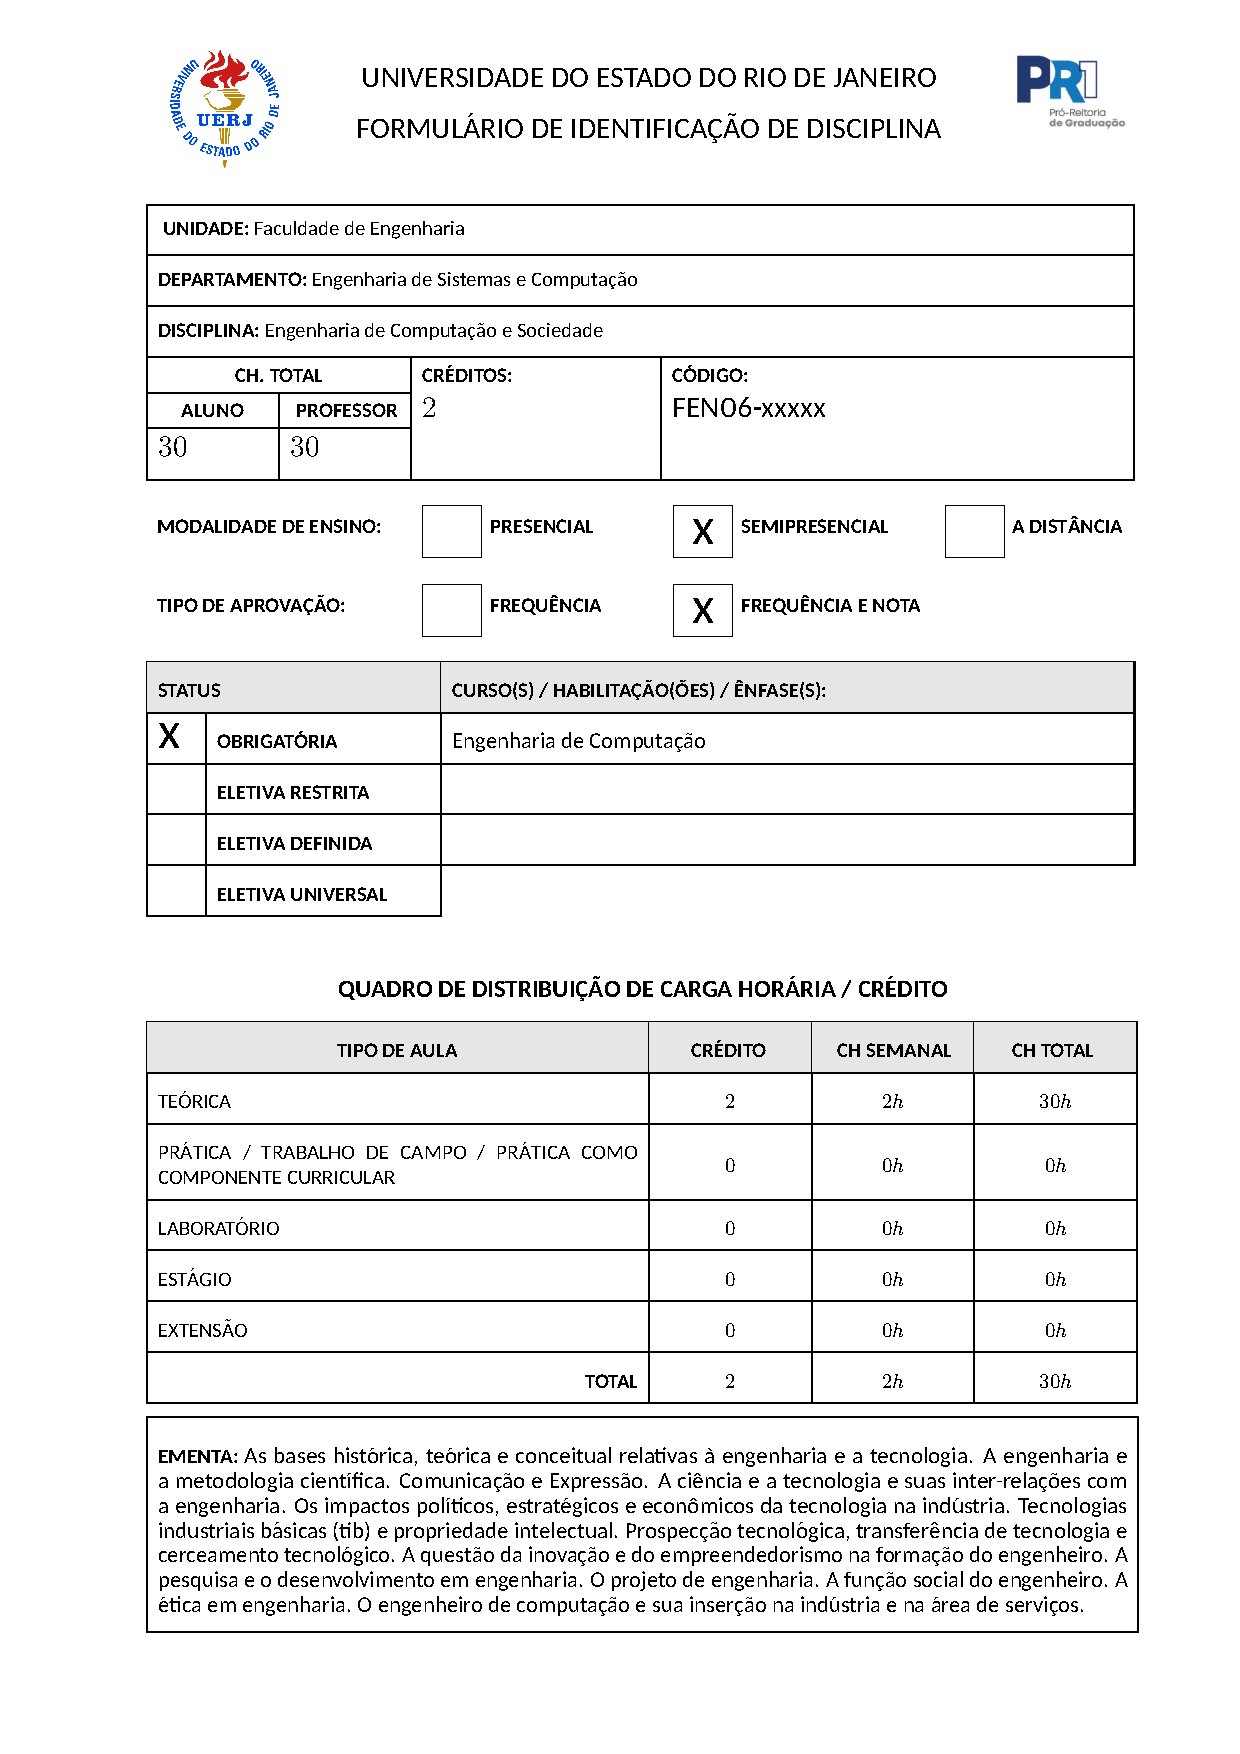
\includepdf[pages=-,addtotoc={1,section,1,{\EngCompSoc},},pagecommand={\thispagestyle{fancy}}]{ementas/EngenhariaDeComputacaoESociedade.pdf}
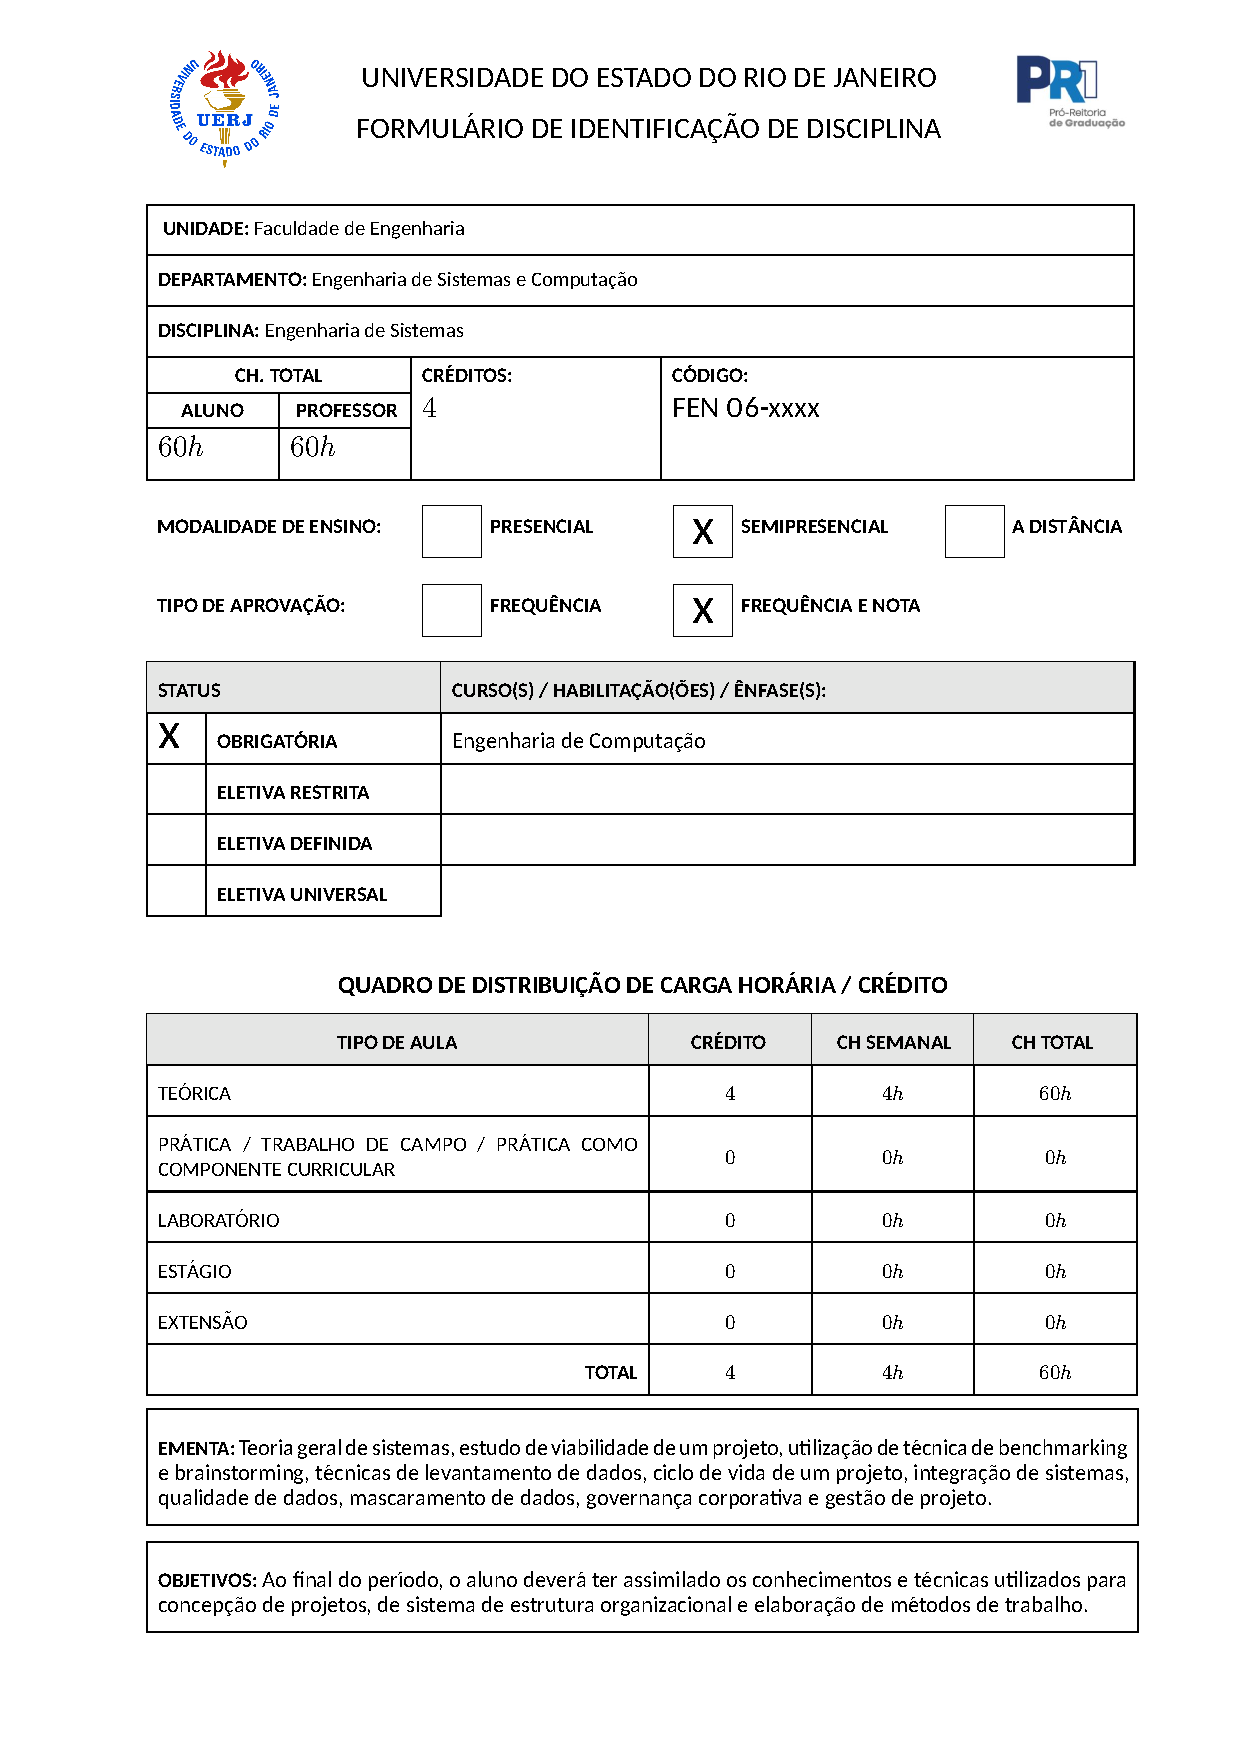
\includepdf[pages=-,addtotoc={1,section,1,{\EngSistA},},pagecommand={\thispagestyle{fancy}}]{ementas/EngenhariaDeSistemas.pdf}
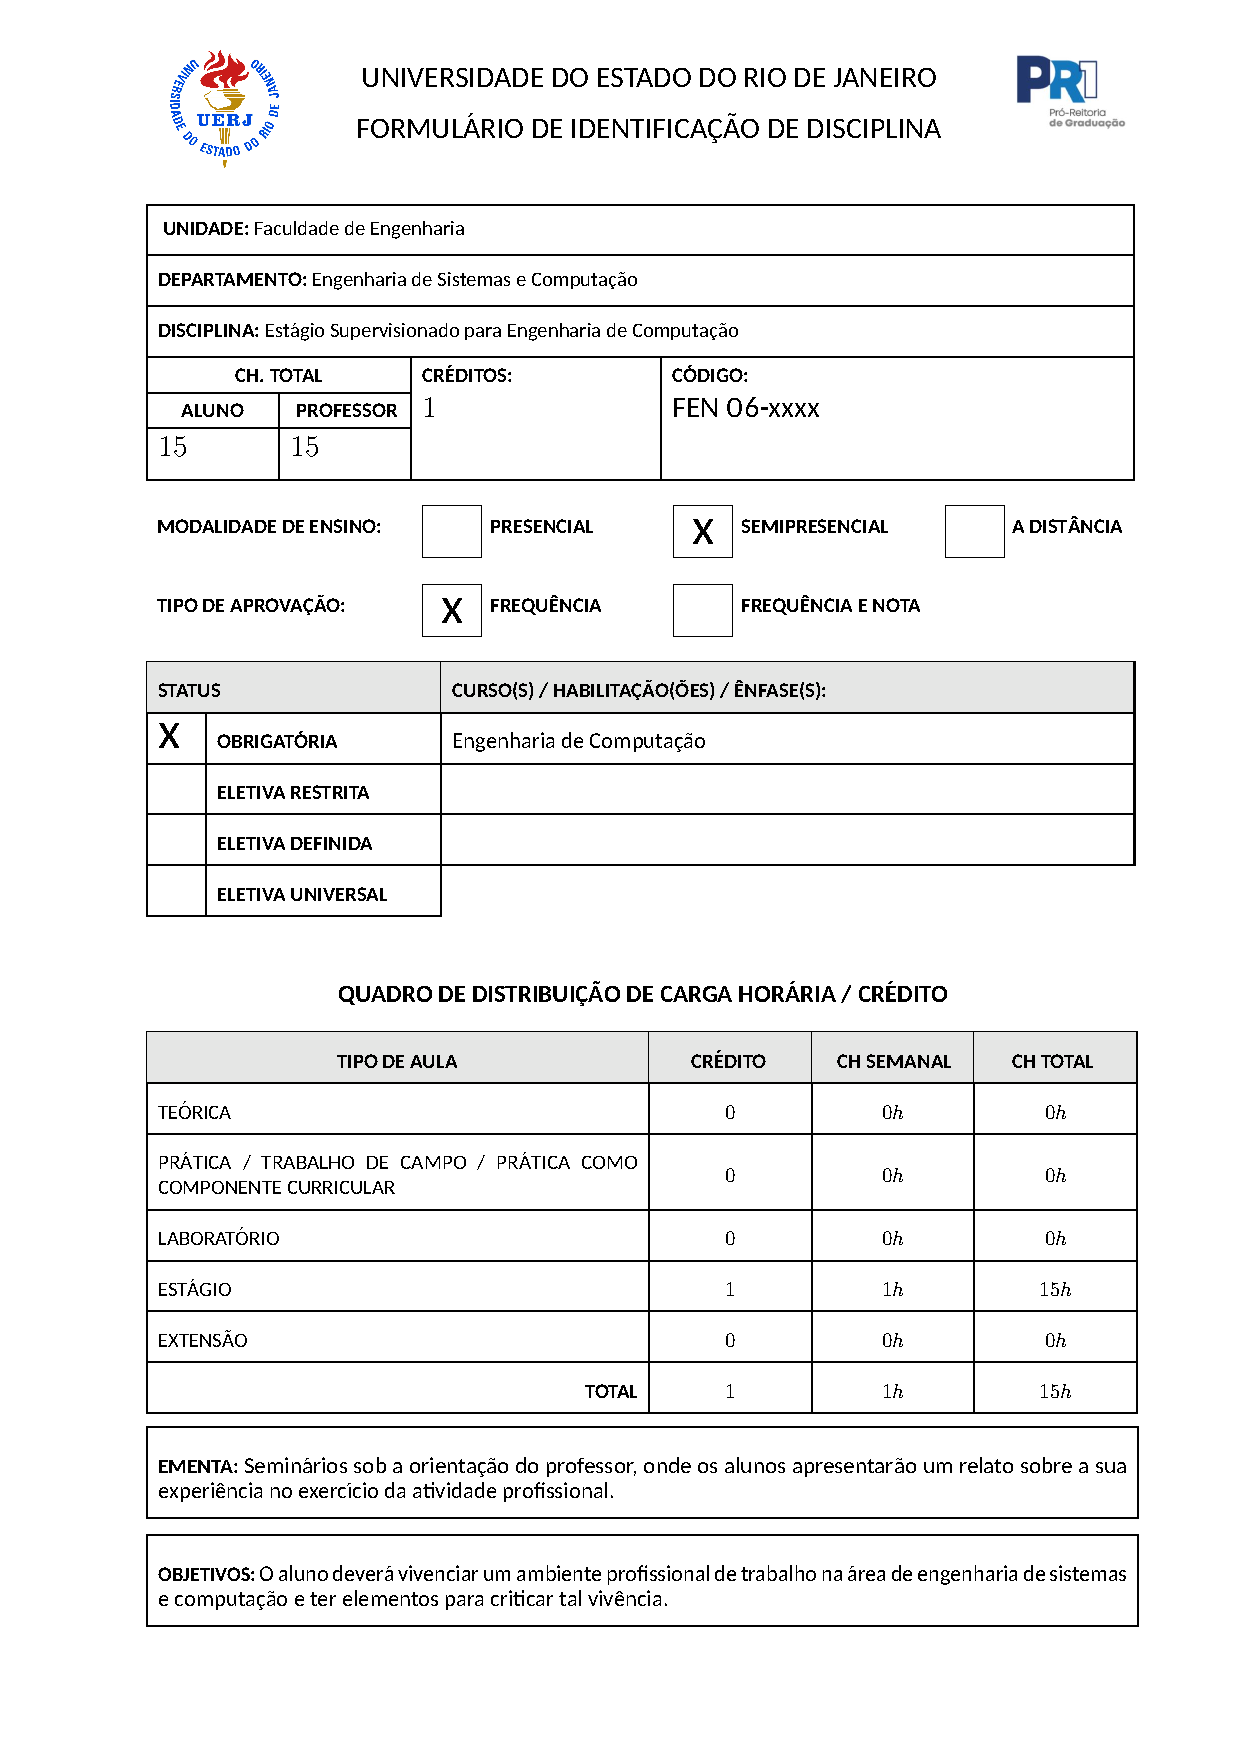
\includepdf[pages=-,addtotoc={1,section,1,{\EstSup},},pagecommand={\thispagestyle{fancy}}]{ementas/EstagioSupervisionadoXIA.pdf}
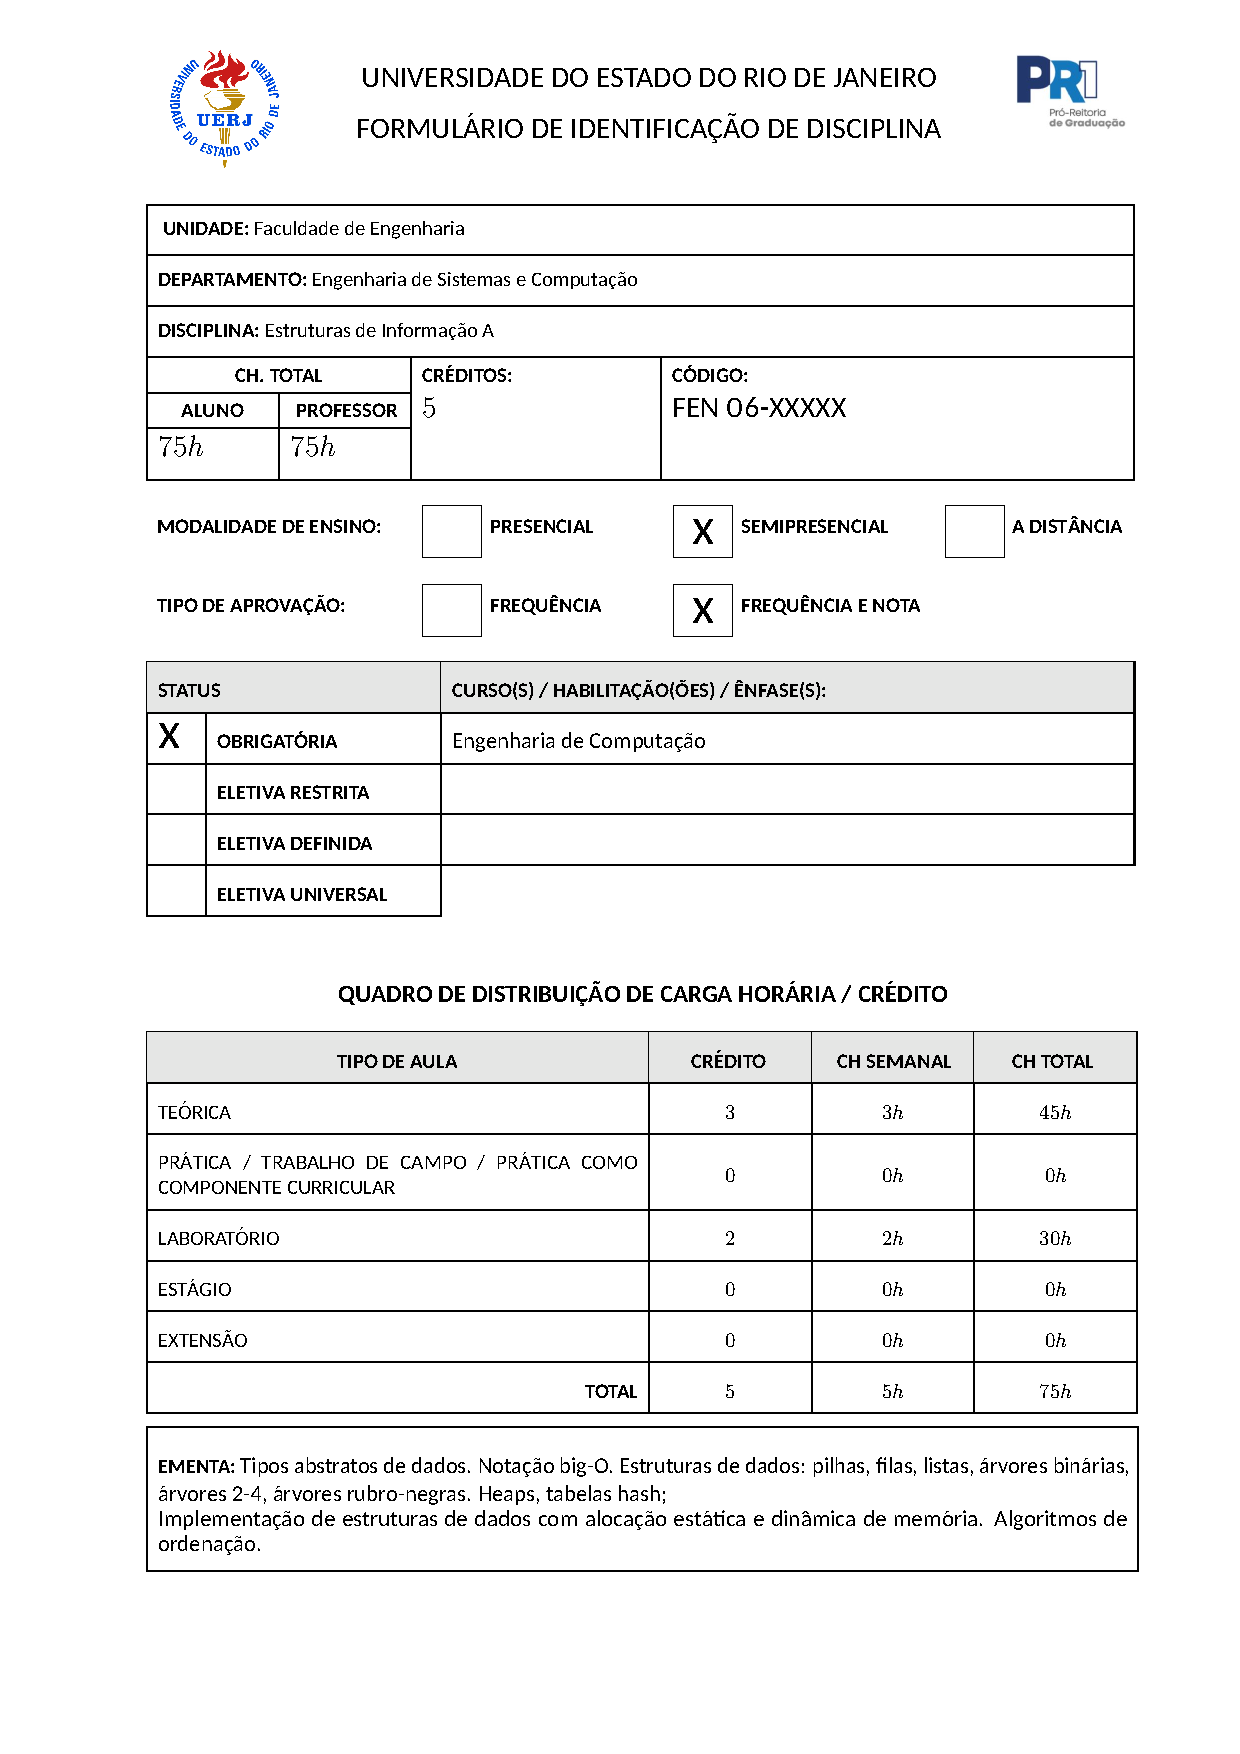
\includepdf[pages=-,addtotoc={1,section,1,{\EstrInf},},pagecommand={\thispagestyle{fancy}}]{ementas/EstruturasDeInformacao.pdf}
\includepdf[pages=-,addtotoc={1,section,1,{\FisEI},},pagecommand={\thispagestyle{fancy}}]{ementasExternas/fisica_experimental_i.pdf}
\includepdf[pages=-,addtotoc={1,section,1,{\FisEII},},pagecommand={\thispagestyle{fancy}}]{ementasExternas/fisica_experimental_ii.pdf}
\includepdf[pages=-,addtotoc={1,section,1,{\FisEIV},},pagecommand={\thispagestyle{fancy}}]{ementasExternas/fisica_experimental_iv.pdf}
\includepdf[pages=-,addtotoc={1,section,1,{\FisI},},pagecommand={\thispagestyle{fancy}}]{ementasExternas/fisica_teorica_i.pdf}
\includepdf[pages=-,addtotoc={1,section,1,{\FisII},},pagecommand={\thispagestyle{fancy}}]{ementasExternas/fisica_teorica_ii.pdf}
\includepdf[pages=-,addtotoc={1,section,1,{\FisIV},},pagecommand={\thispagestyle{fancy}}]{ementasExternas/fisica_teorica_iv.pdf}
% Eletromagnetismo Básico Teórico era 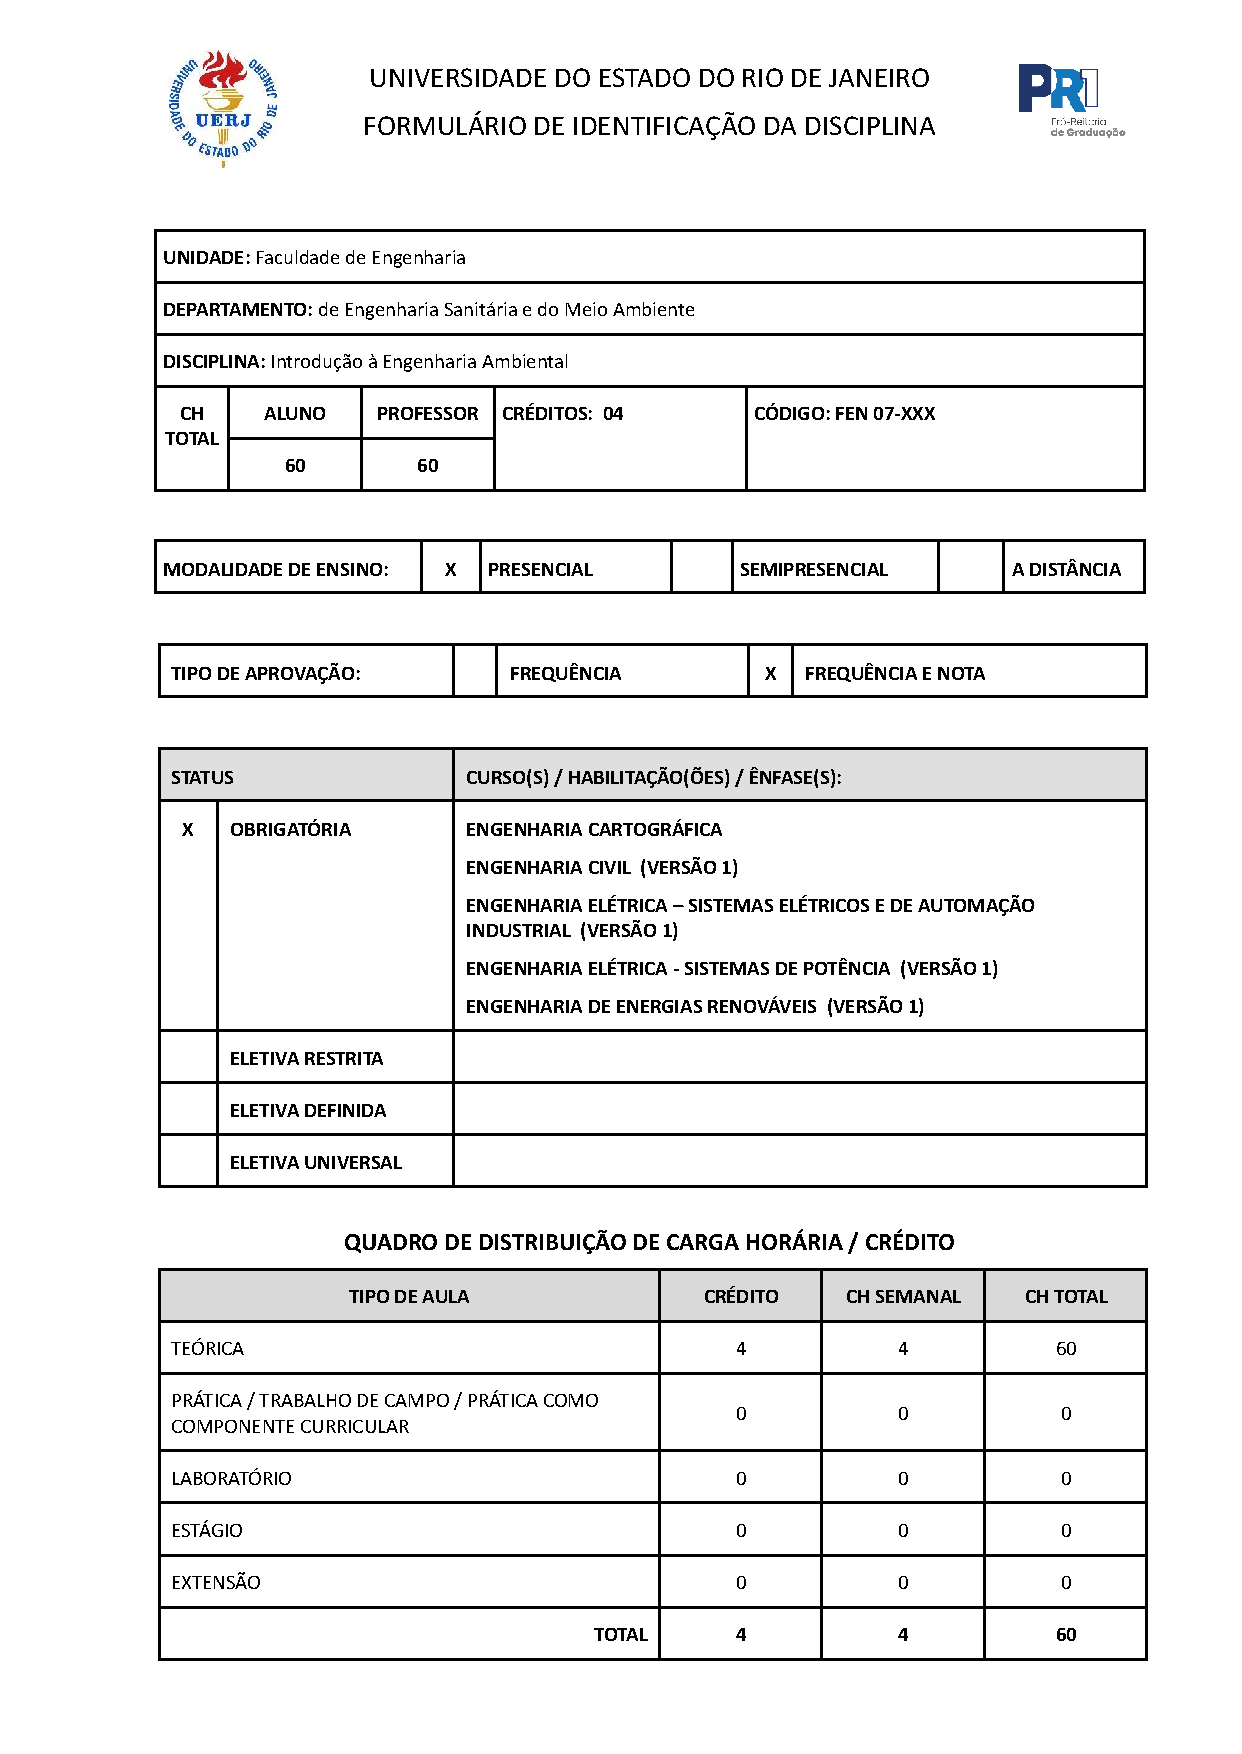
\includepdf[pages=-,addtotoc={1,section,1,{\IntAmb},},pagecommand={\thispagestyle{fancy}}]{ementasExternas/Introducao_a_Engenharia_Ambiental.pdf}
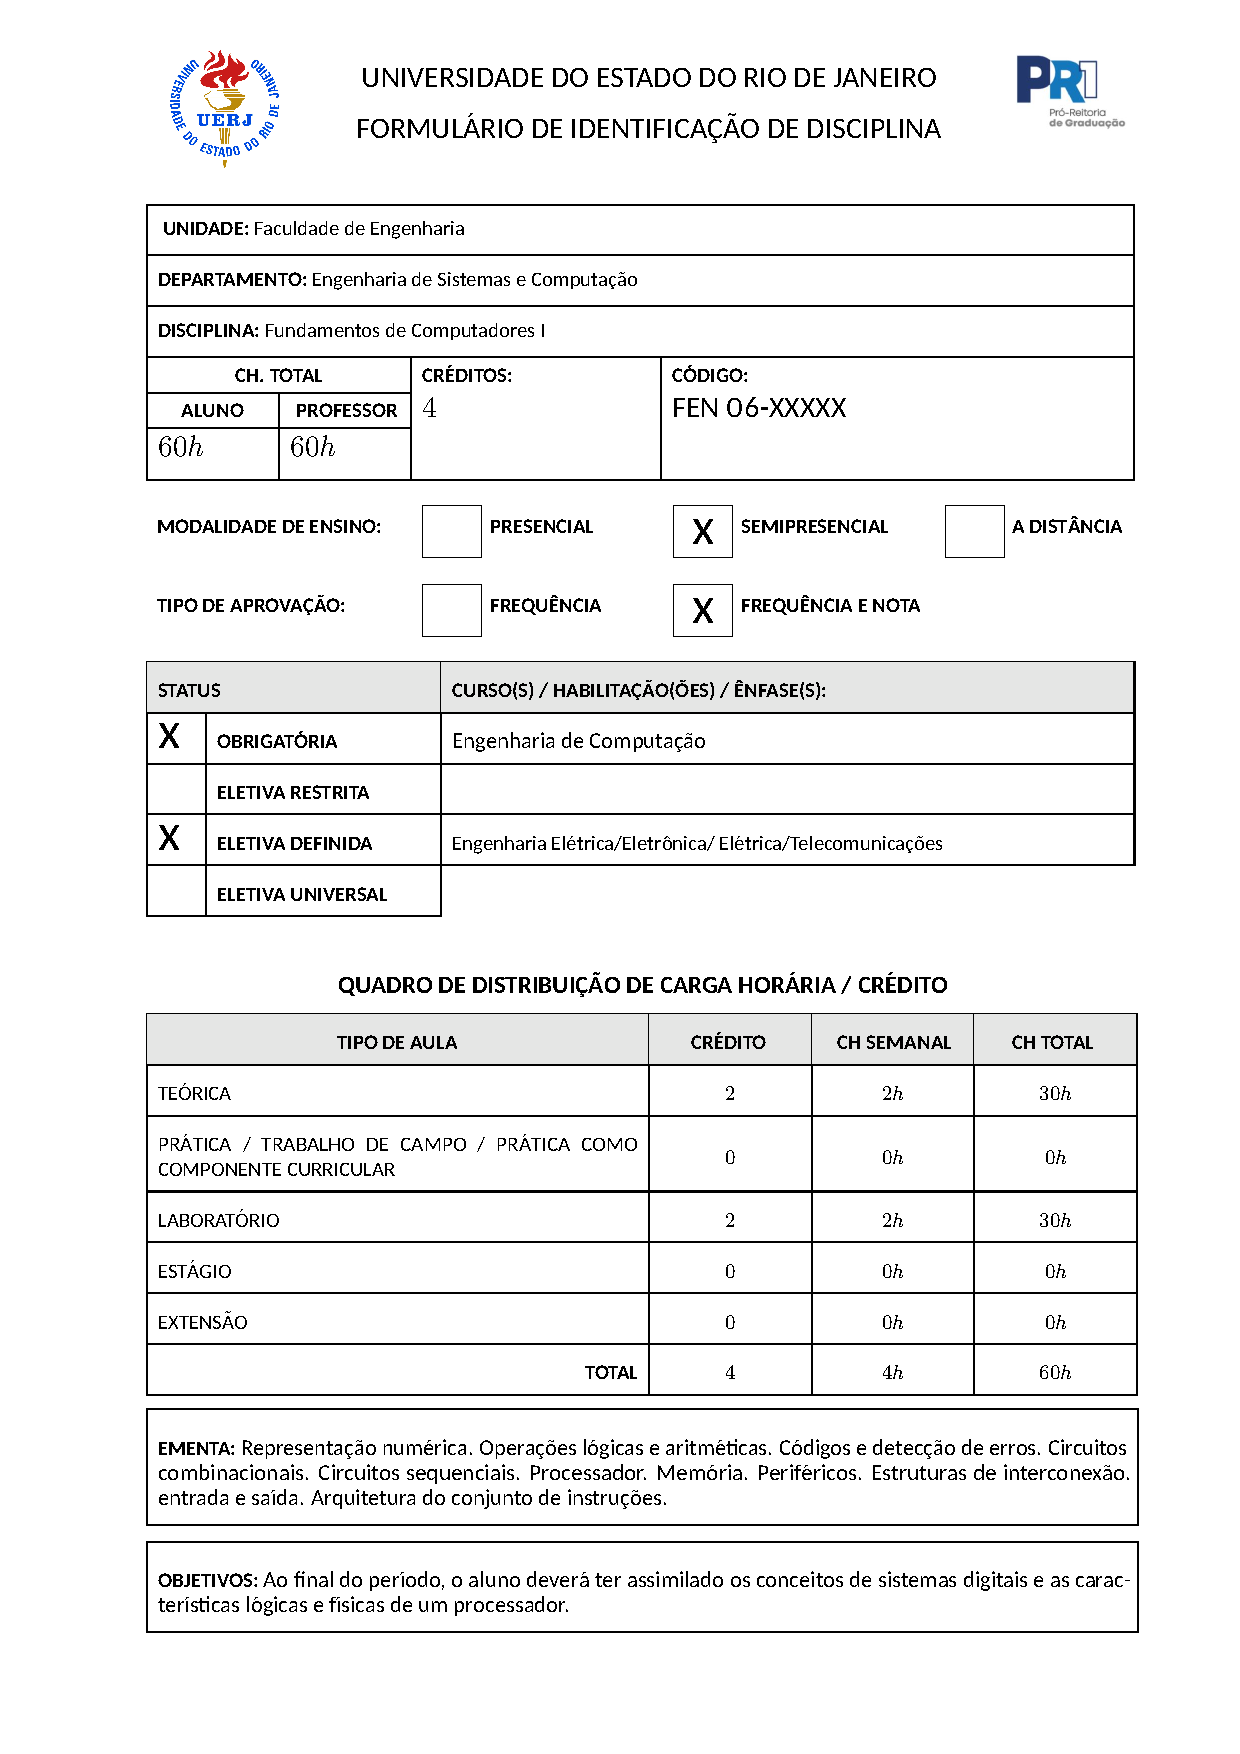
\includepdf[pages=-,addtotoc={1,section,1,{\FundComp},},pagecommand={\thispagestyle{fancy}}]{ementas/FundamentosDeComputadores.pdf}
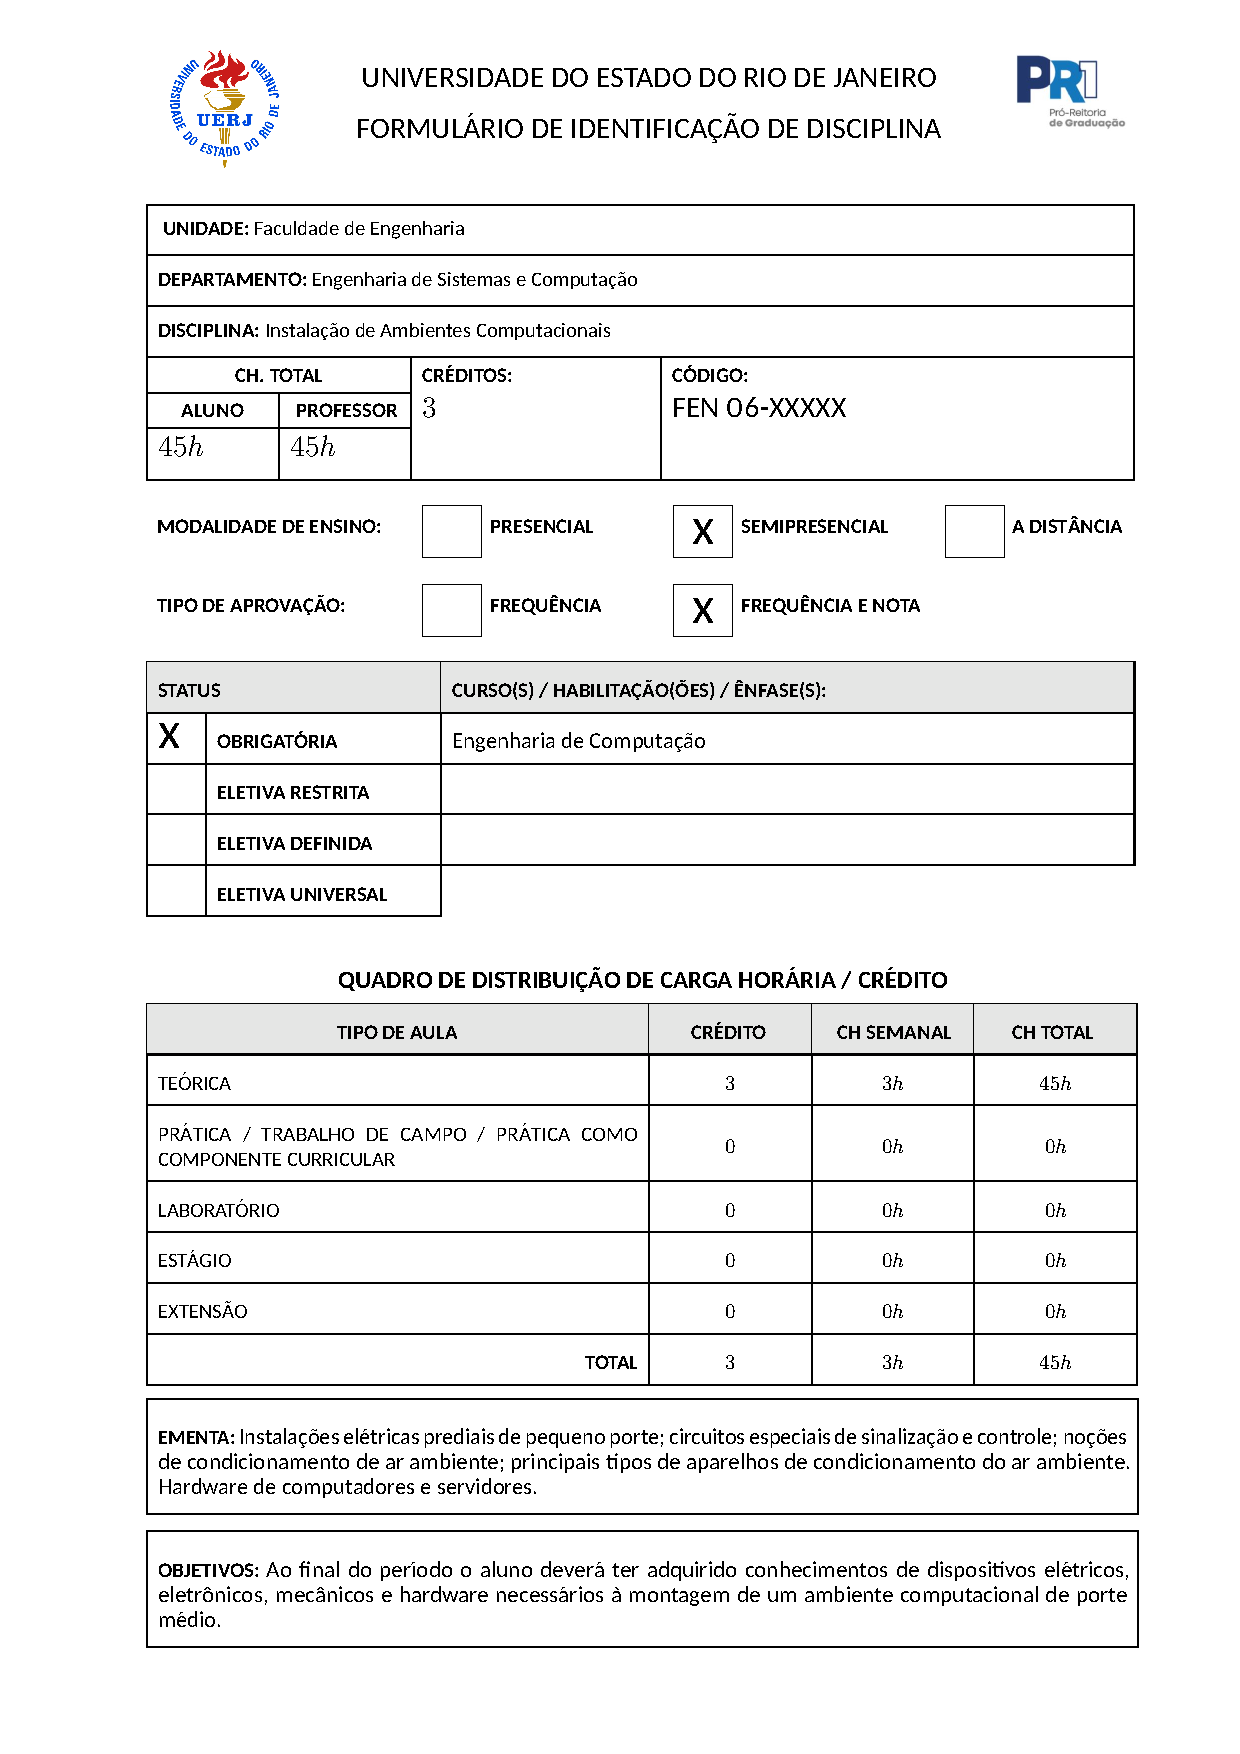
\includepdf[pages=-,addtotoc={1,section,1,{\Instala},},pagecommand={\thispagestyle{fancy}}]{ementas/instalacao_de_ambientes_computacionais.pdf}
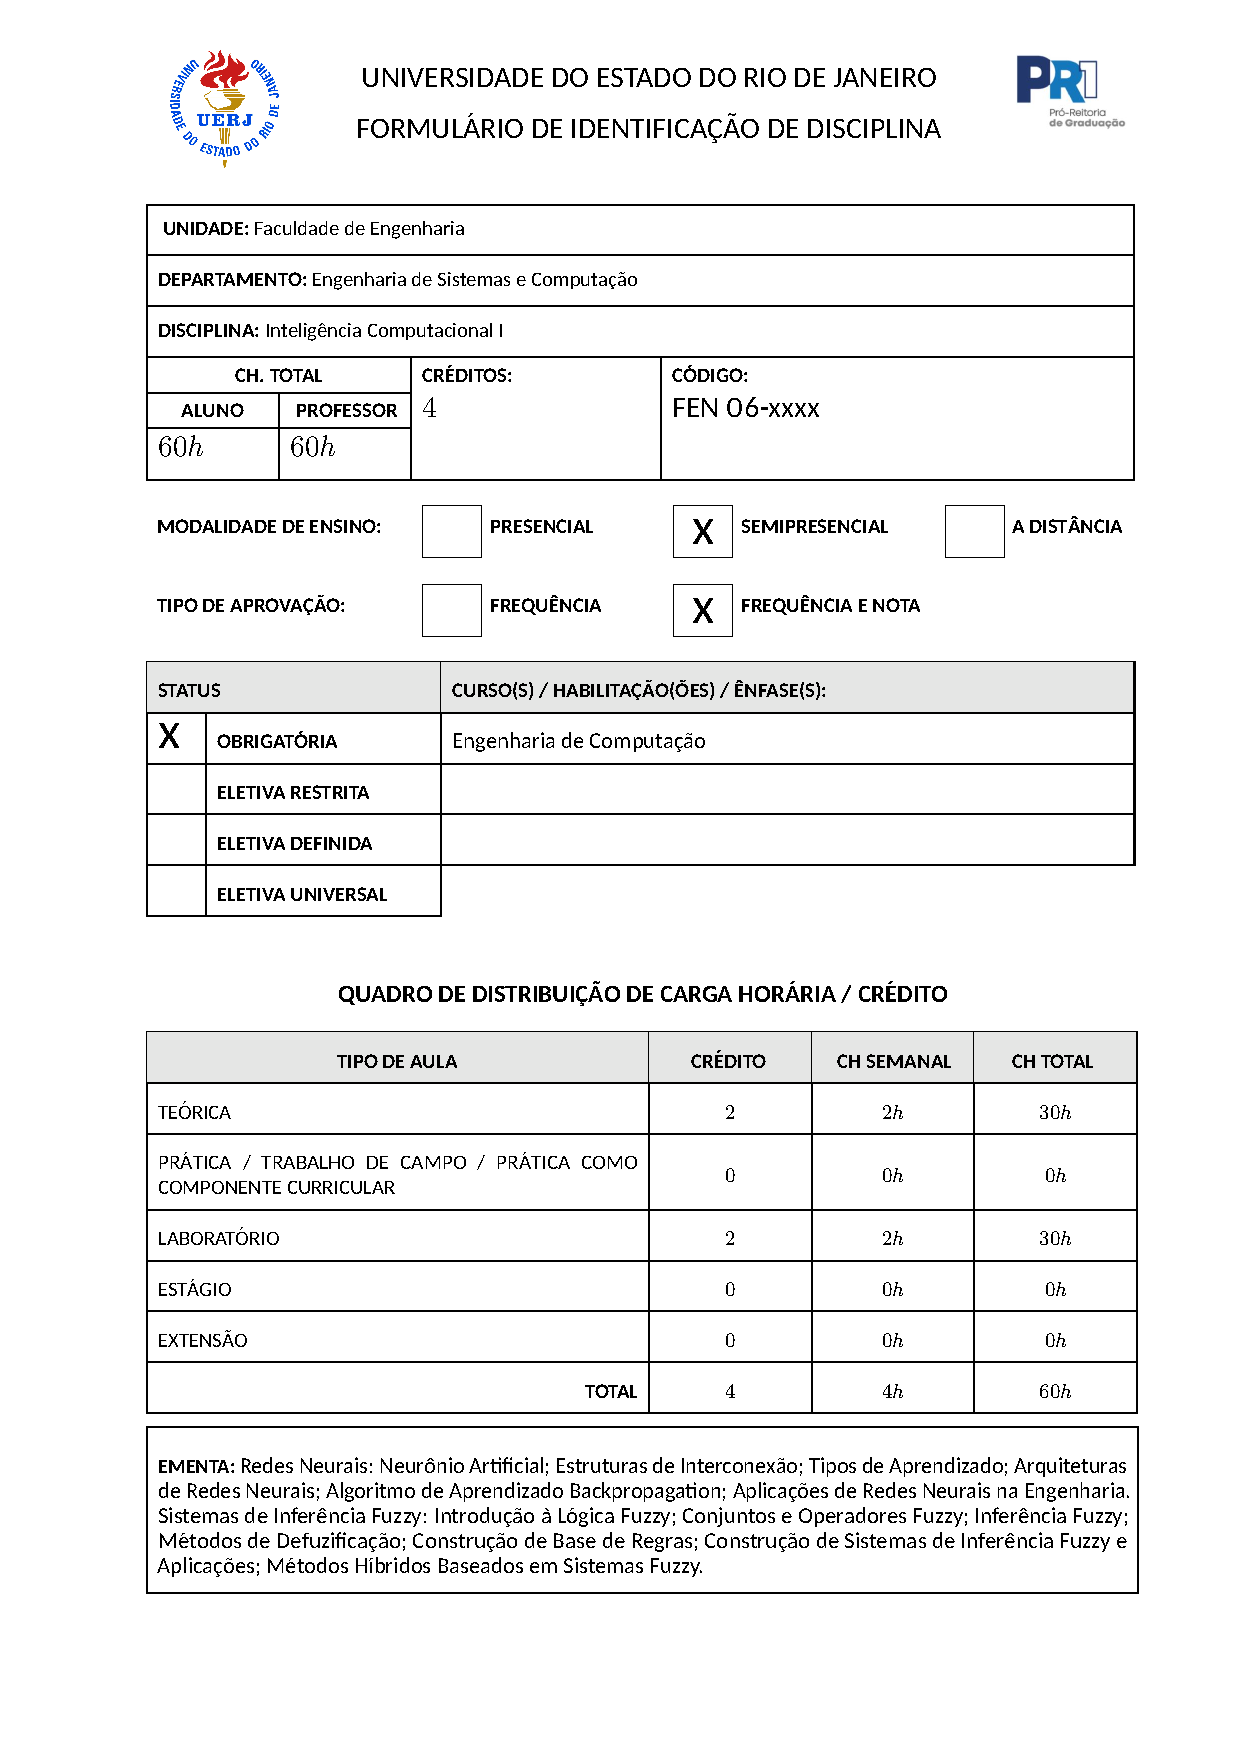
\includepdf[pages=-,addtotoc={1,section,1,{\IC},},pagecommand={\thispagestyle{fancy}}]{ementas/InteligenciaComputacional1.pdf}
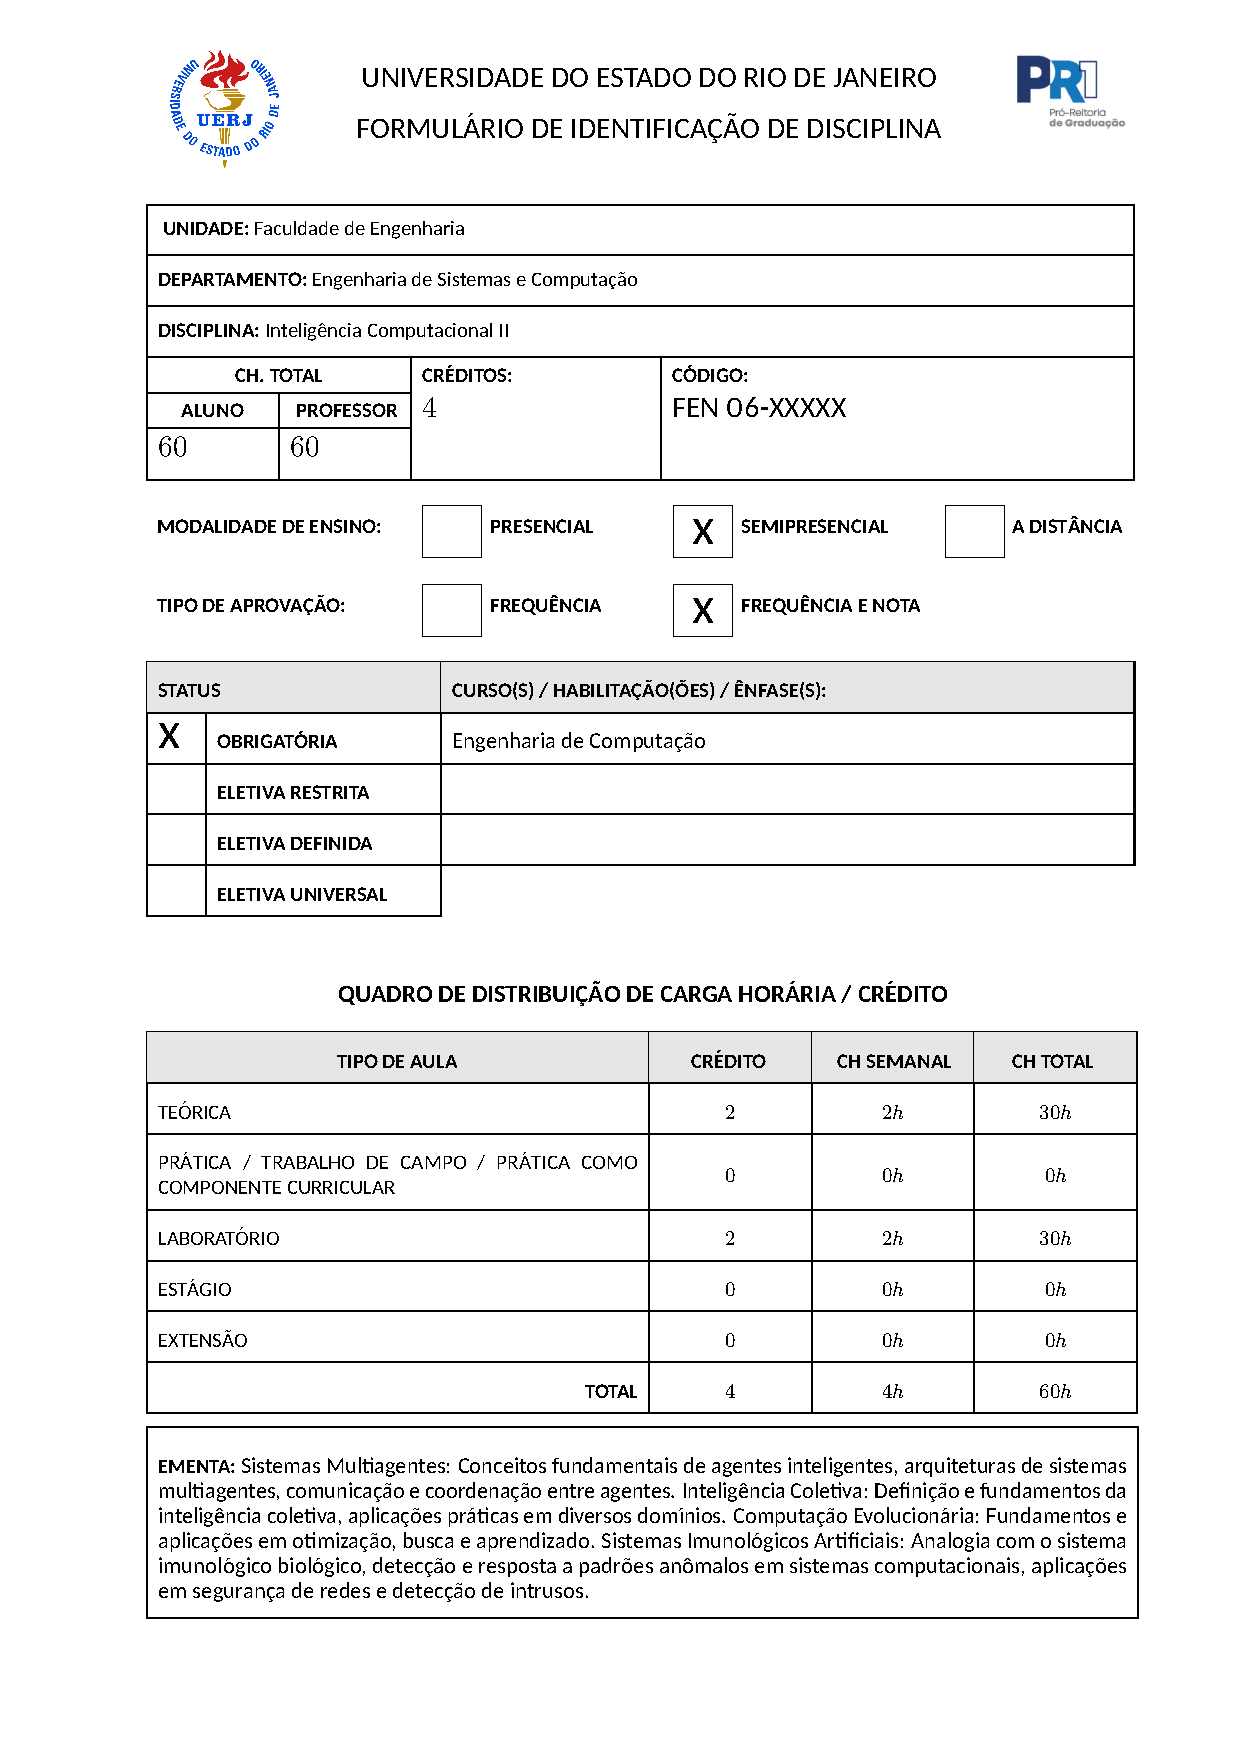
\includepdf[pages=-,addtotoc={1,section,1,{\ICII},},pagecommand={\thispagestyle{fancy}}]{ementas/InteligenciaComputacional2.pdf}
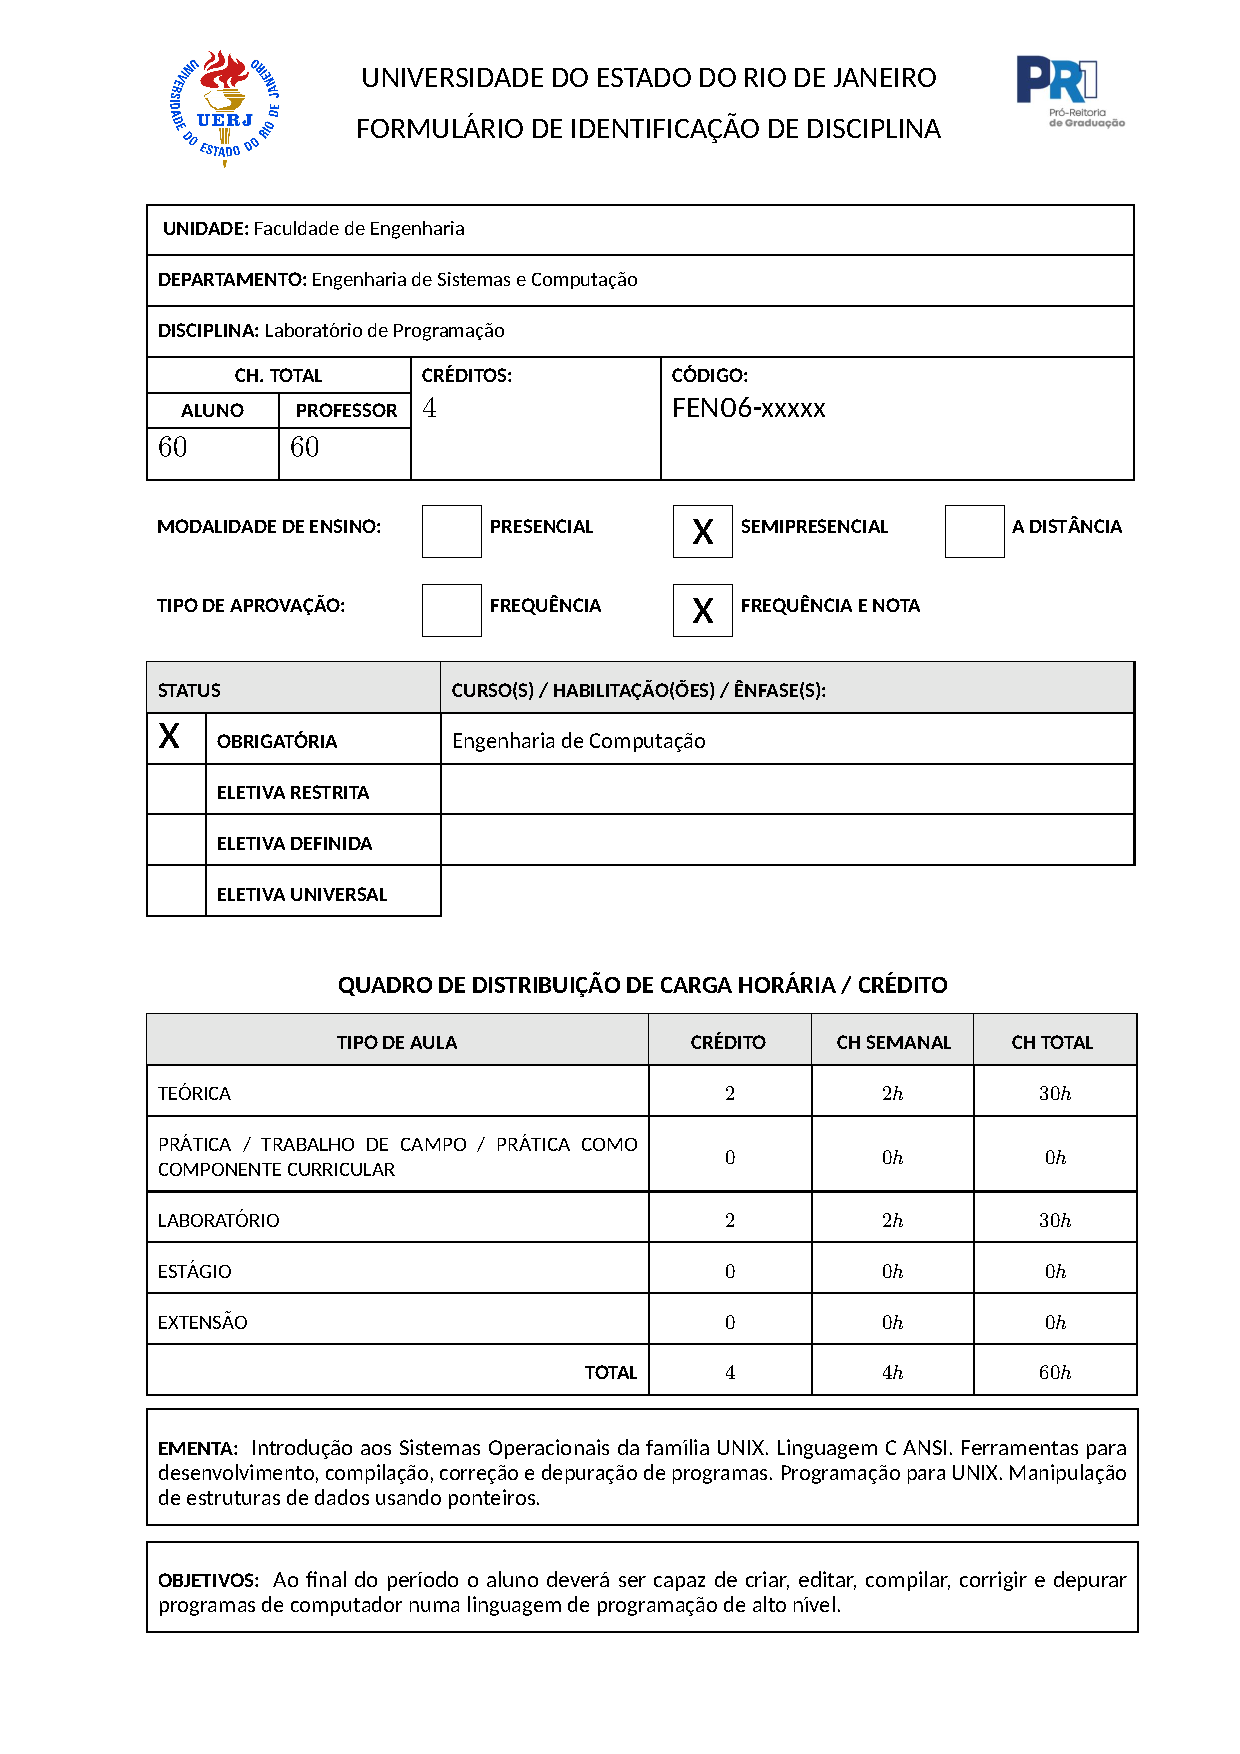
\includepdf[pages=-,addtotoc={1,section,1,{\LabProgA},},pagecommand={\thispagestyle{fancy}}]{ementas/LaboratorioDeProgramacaoA.pdf}
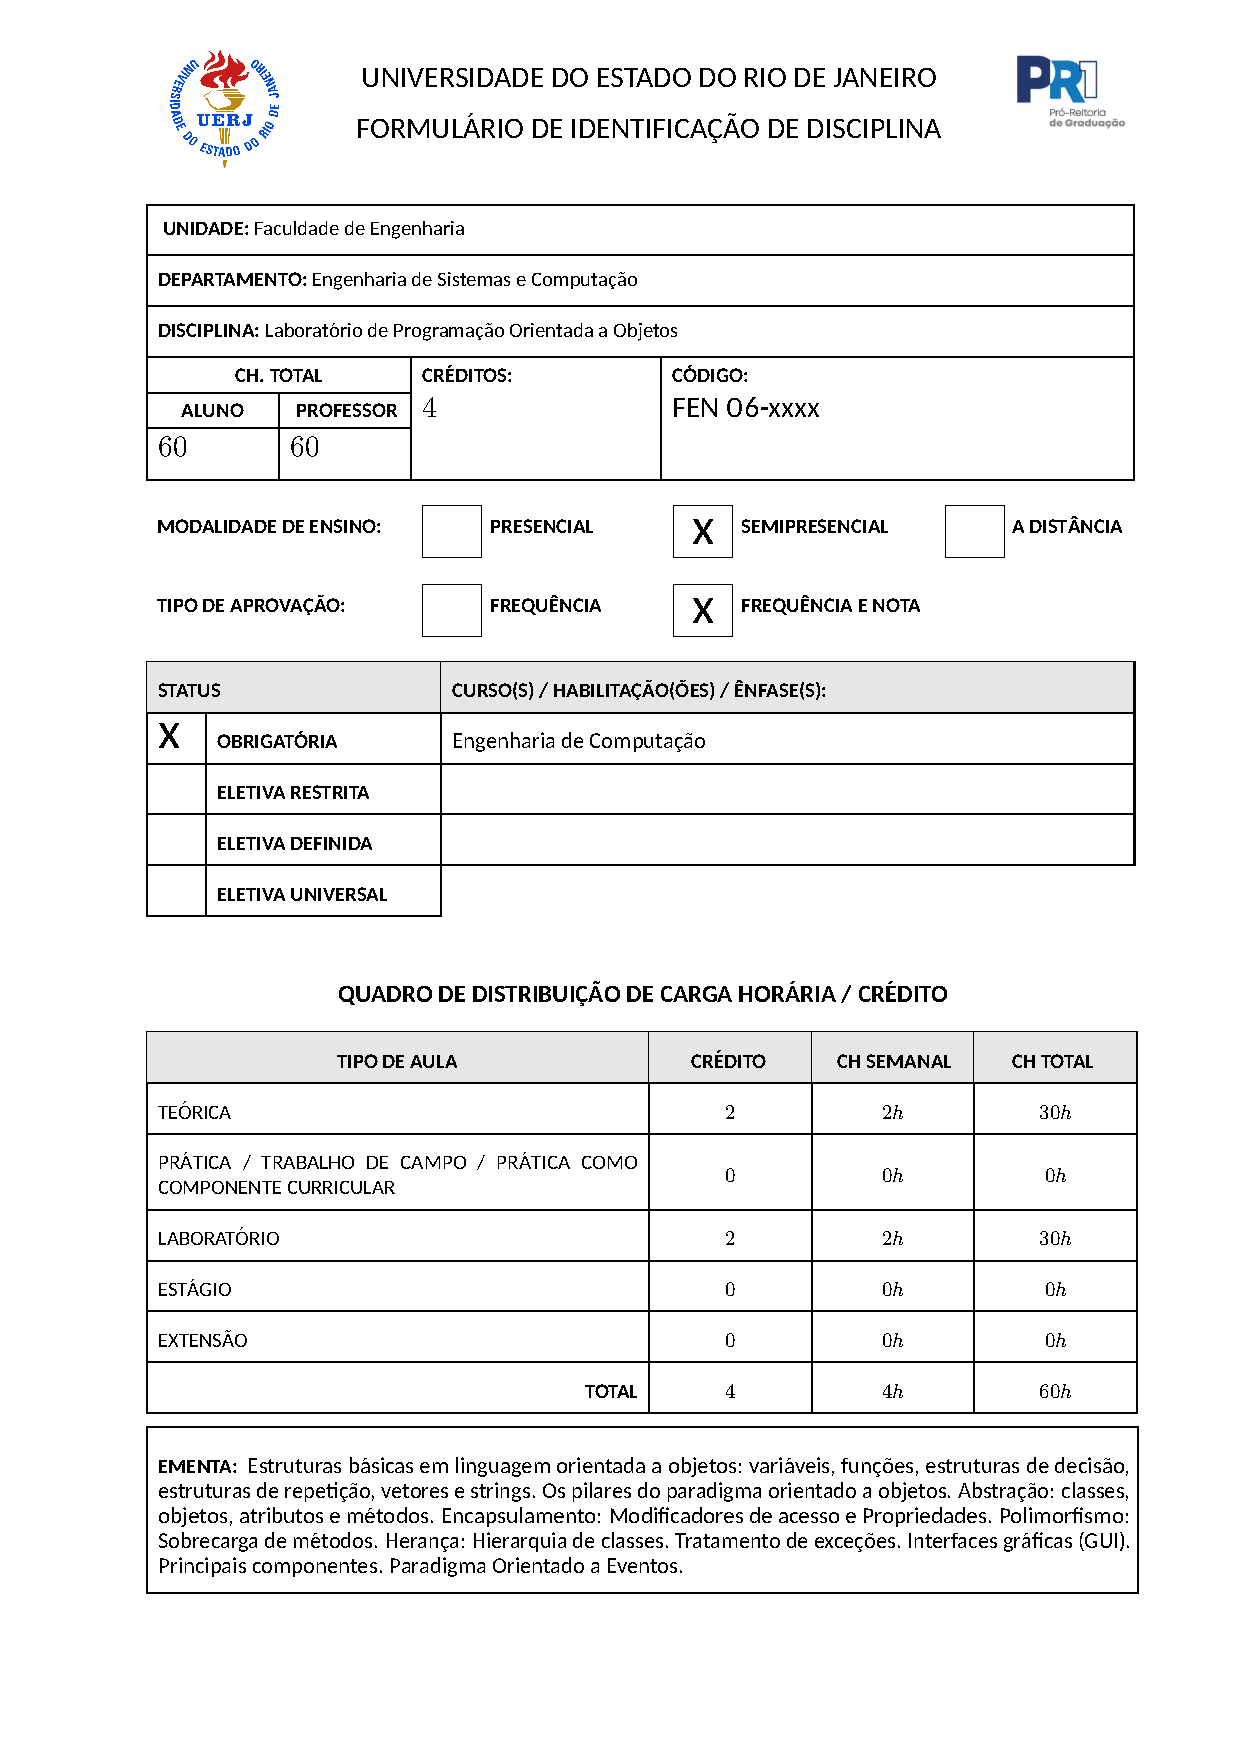
\includepdf[pages=-,addtotoc={1,section,1,{\LabProgPOO},},pagecommand={\thispagestyle{fancy}}]{ementas/LaboratorioDeProgramacaoB.pdf}
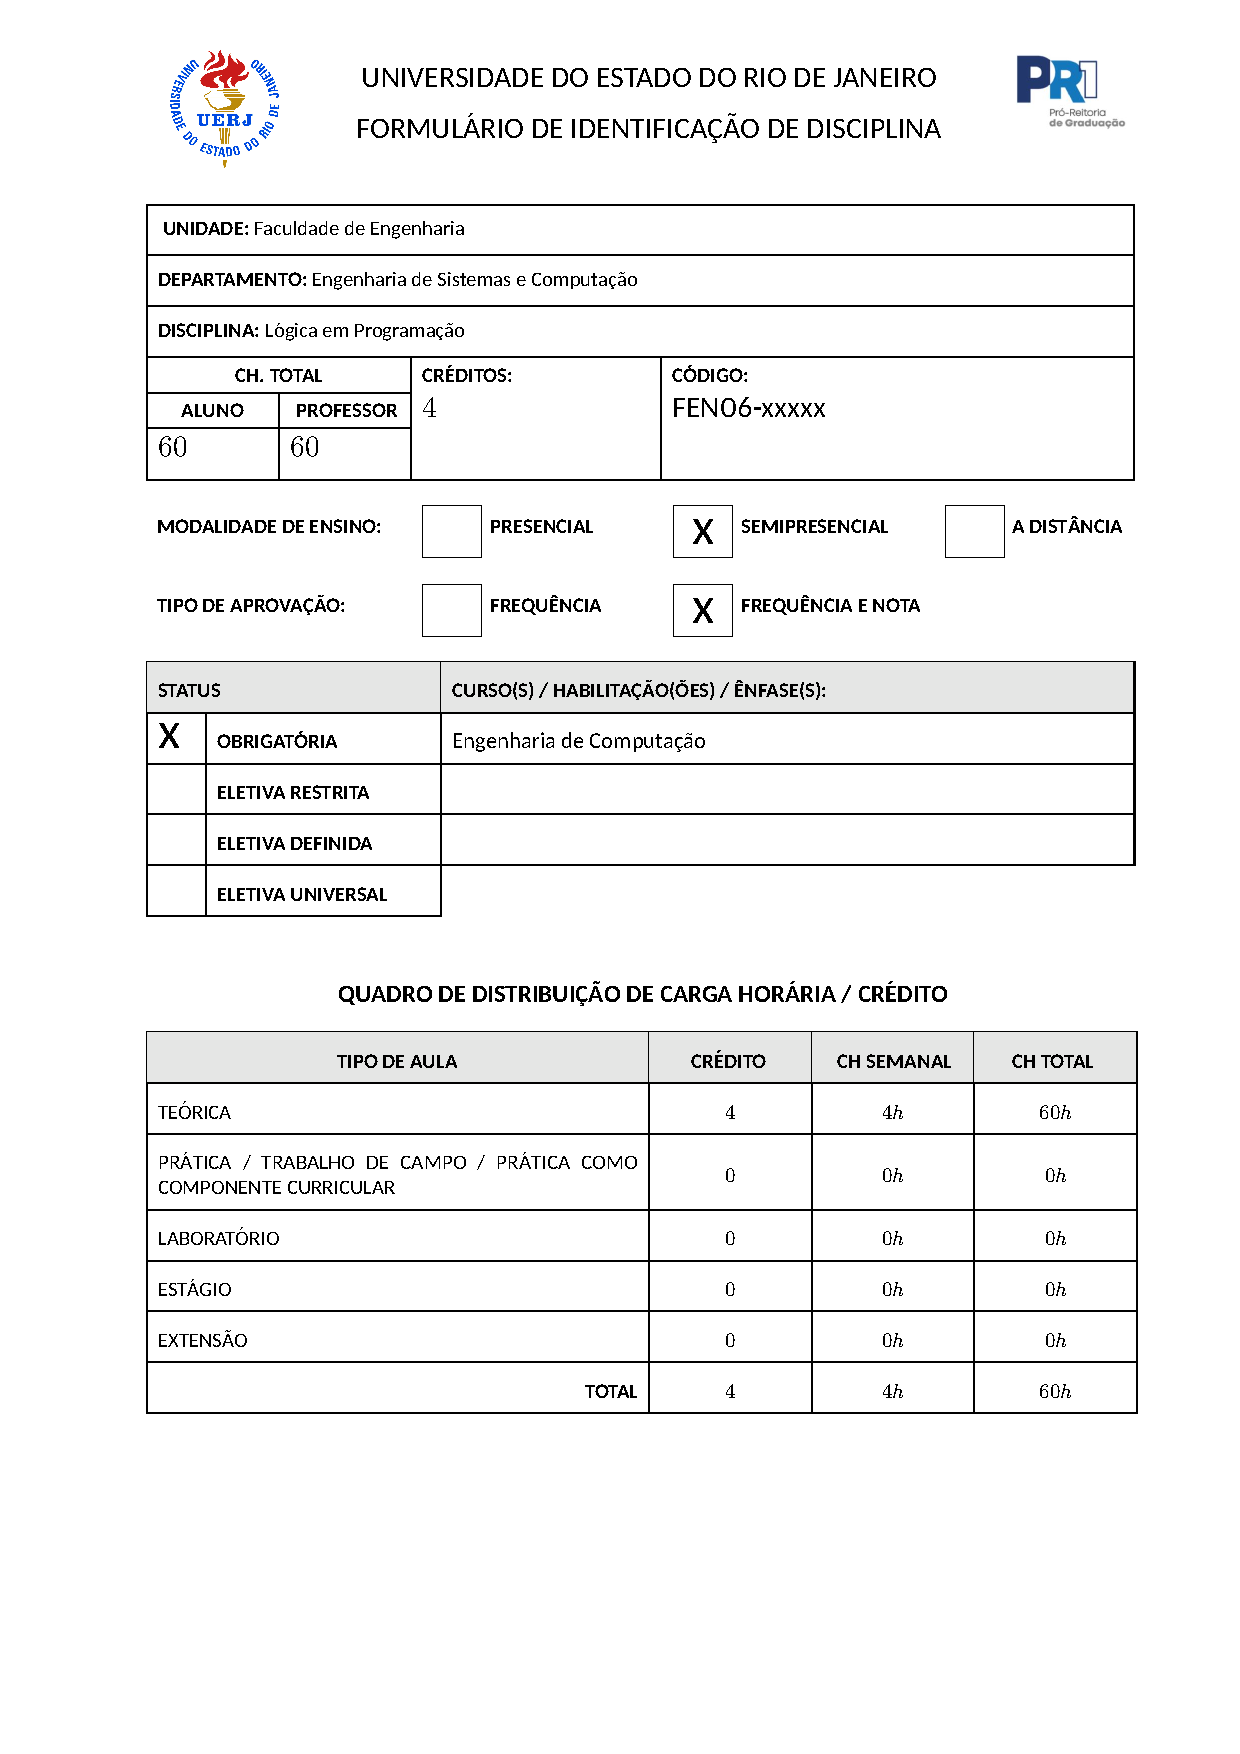
\includepdf[pages=-,addtotoc={1,section,1,{\LogProg},},pagecommand={\thispagestyle{fancy}}]{ementas/LogicaEmProgramacao.pdf}
\includepdf[pages=-,addtotoc={1,section,1,{\MacroEco},},pagecommand={\thispagestyle{fancy}}]{ementasExternas/macroeconomia.pdf} % Macroeconomia
% Materiais Elétricos e Eletrônicos era 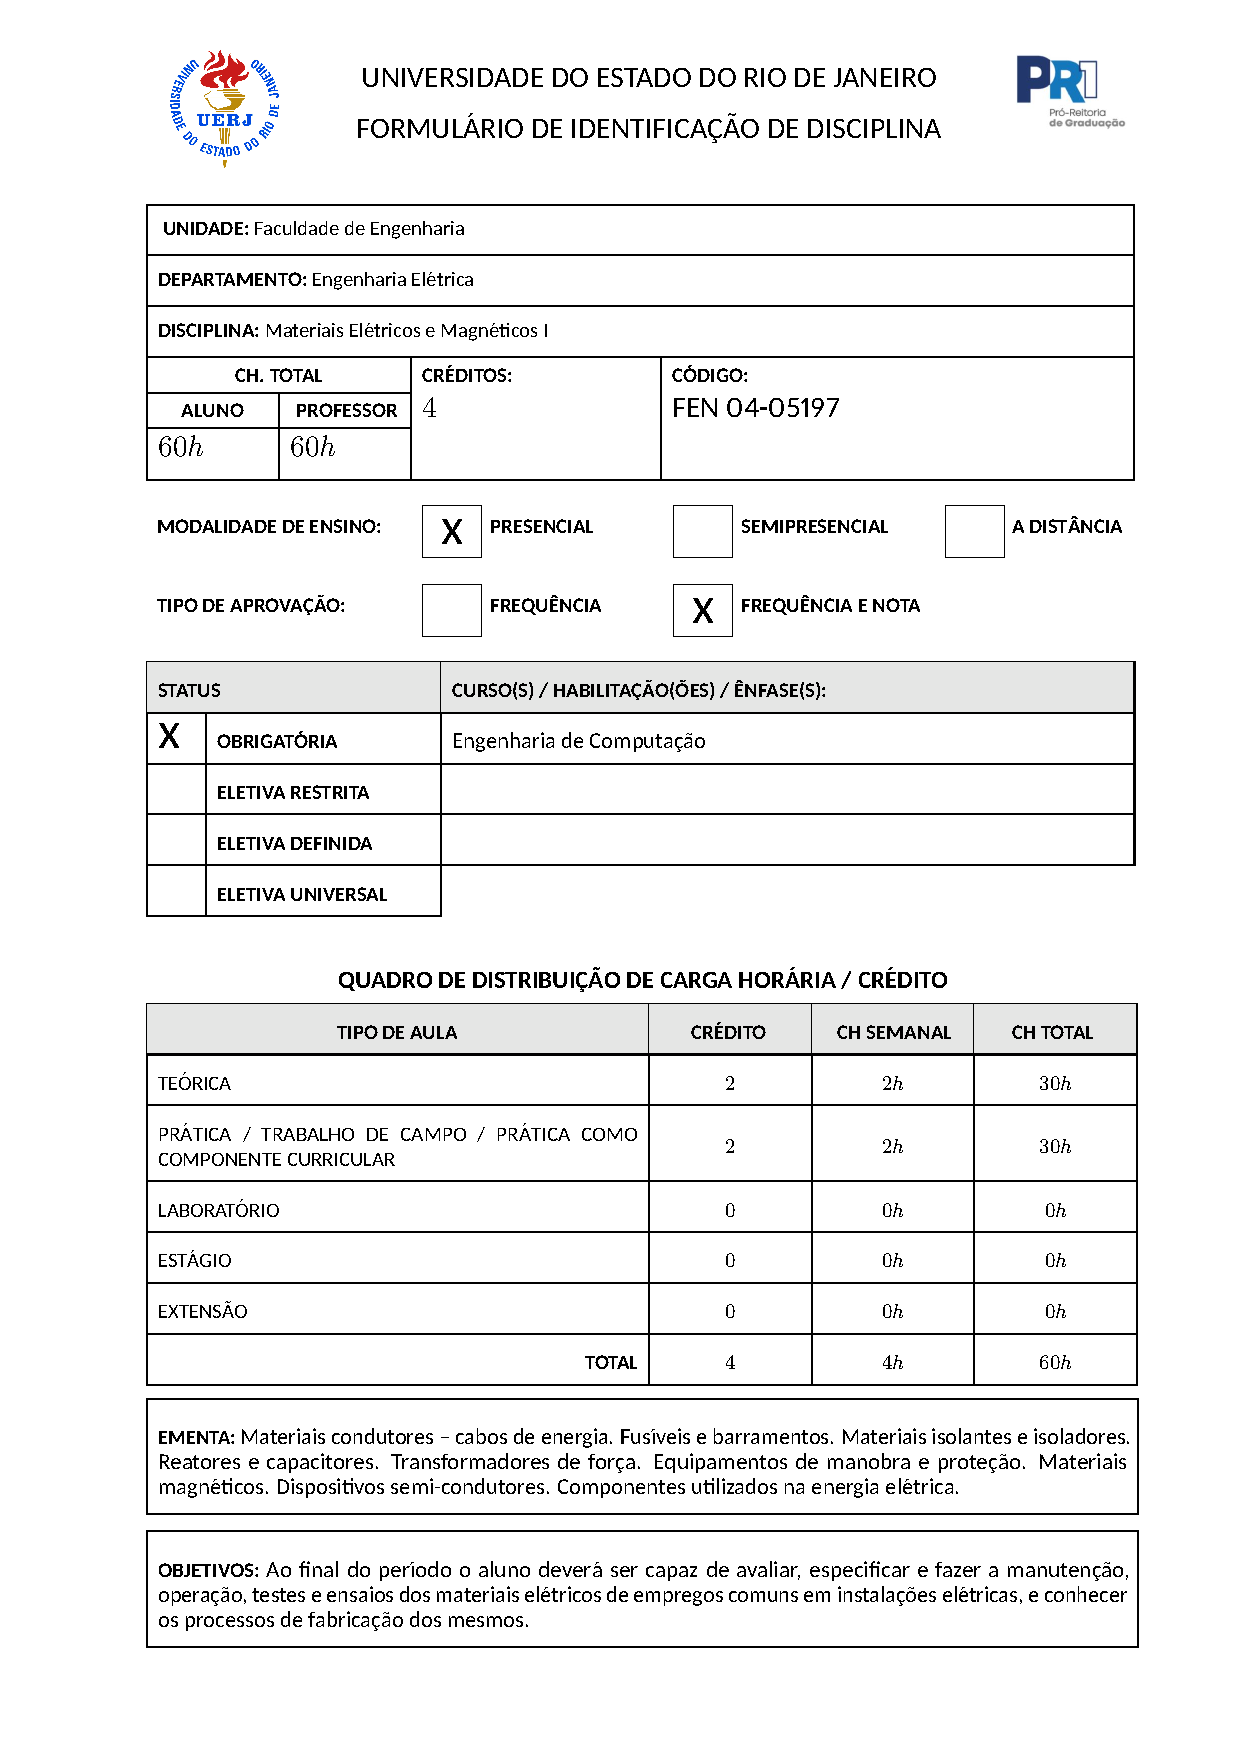
\includepdf[pages=-,addtotoc={1,section,1,{\MatEle},},pagecommand={\thispagestyle{fancy}}]{ementas/MateriaisEletricosEMagneticos.pdf}
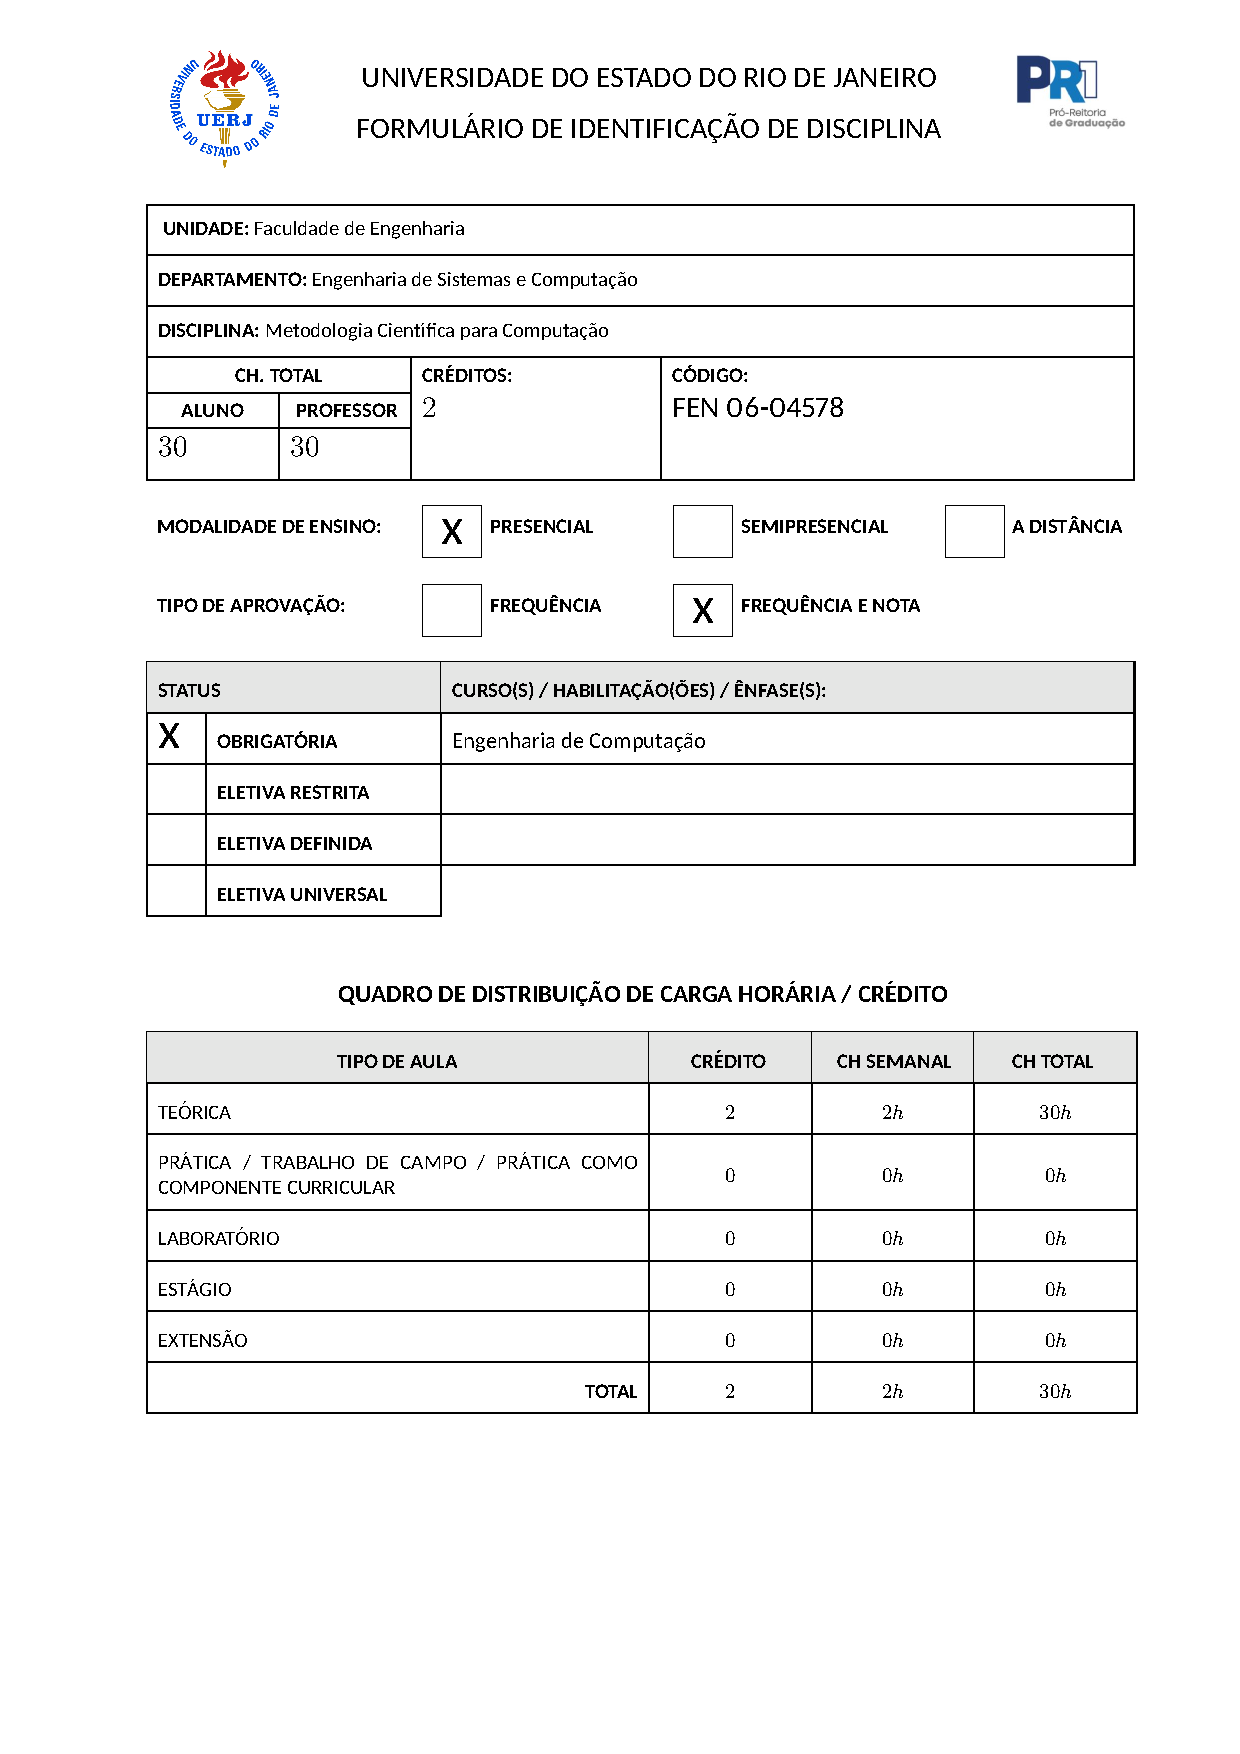
\includepdf[pages=-,addtotoc={1,section,1,{\ProjA},},pagecommand={\thispagestyle{fancy}}]{ementas/ProjetoXIA.pdf} %  Metodo de Projeto 
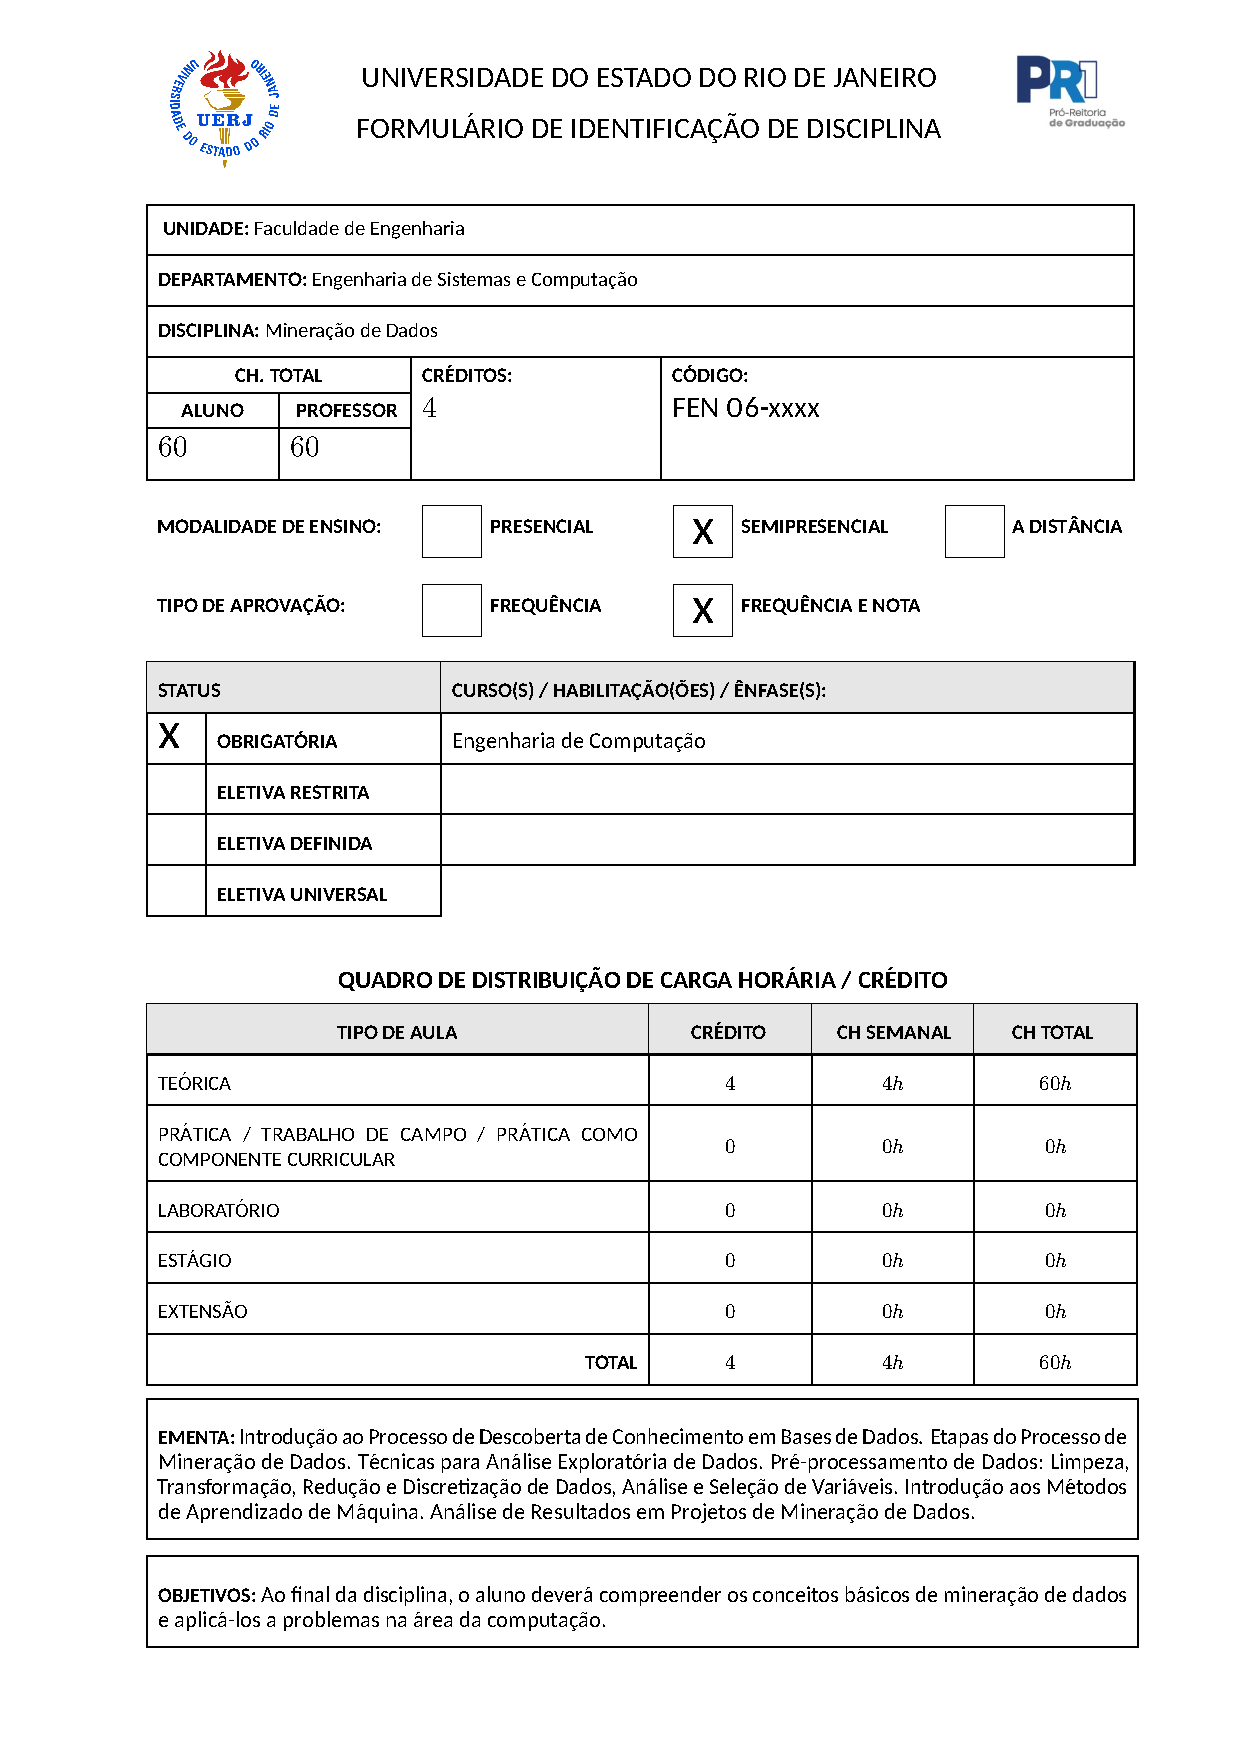
\includepdf[pages=-,addtotoc={1,section,1,{\MineraDados},},pagecommand={\thispagestyle{fancy}}]{ementas/MineracaoDeDados.pdf}
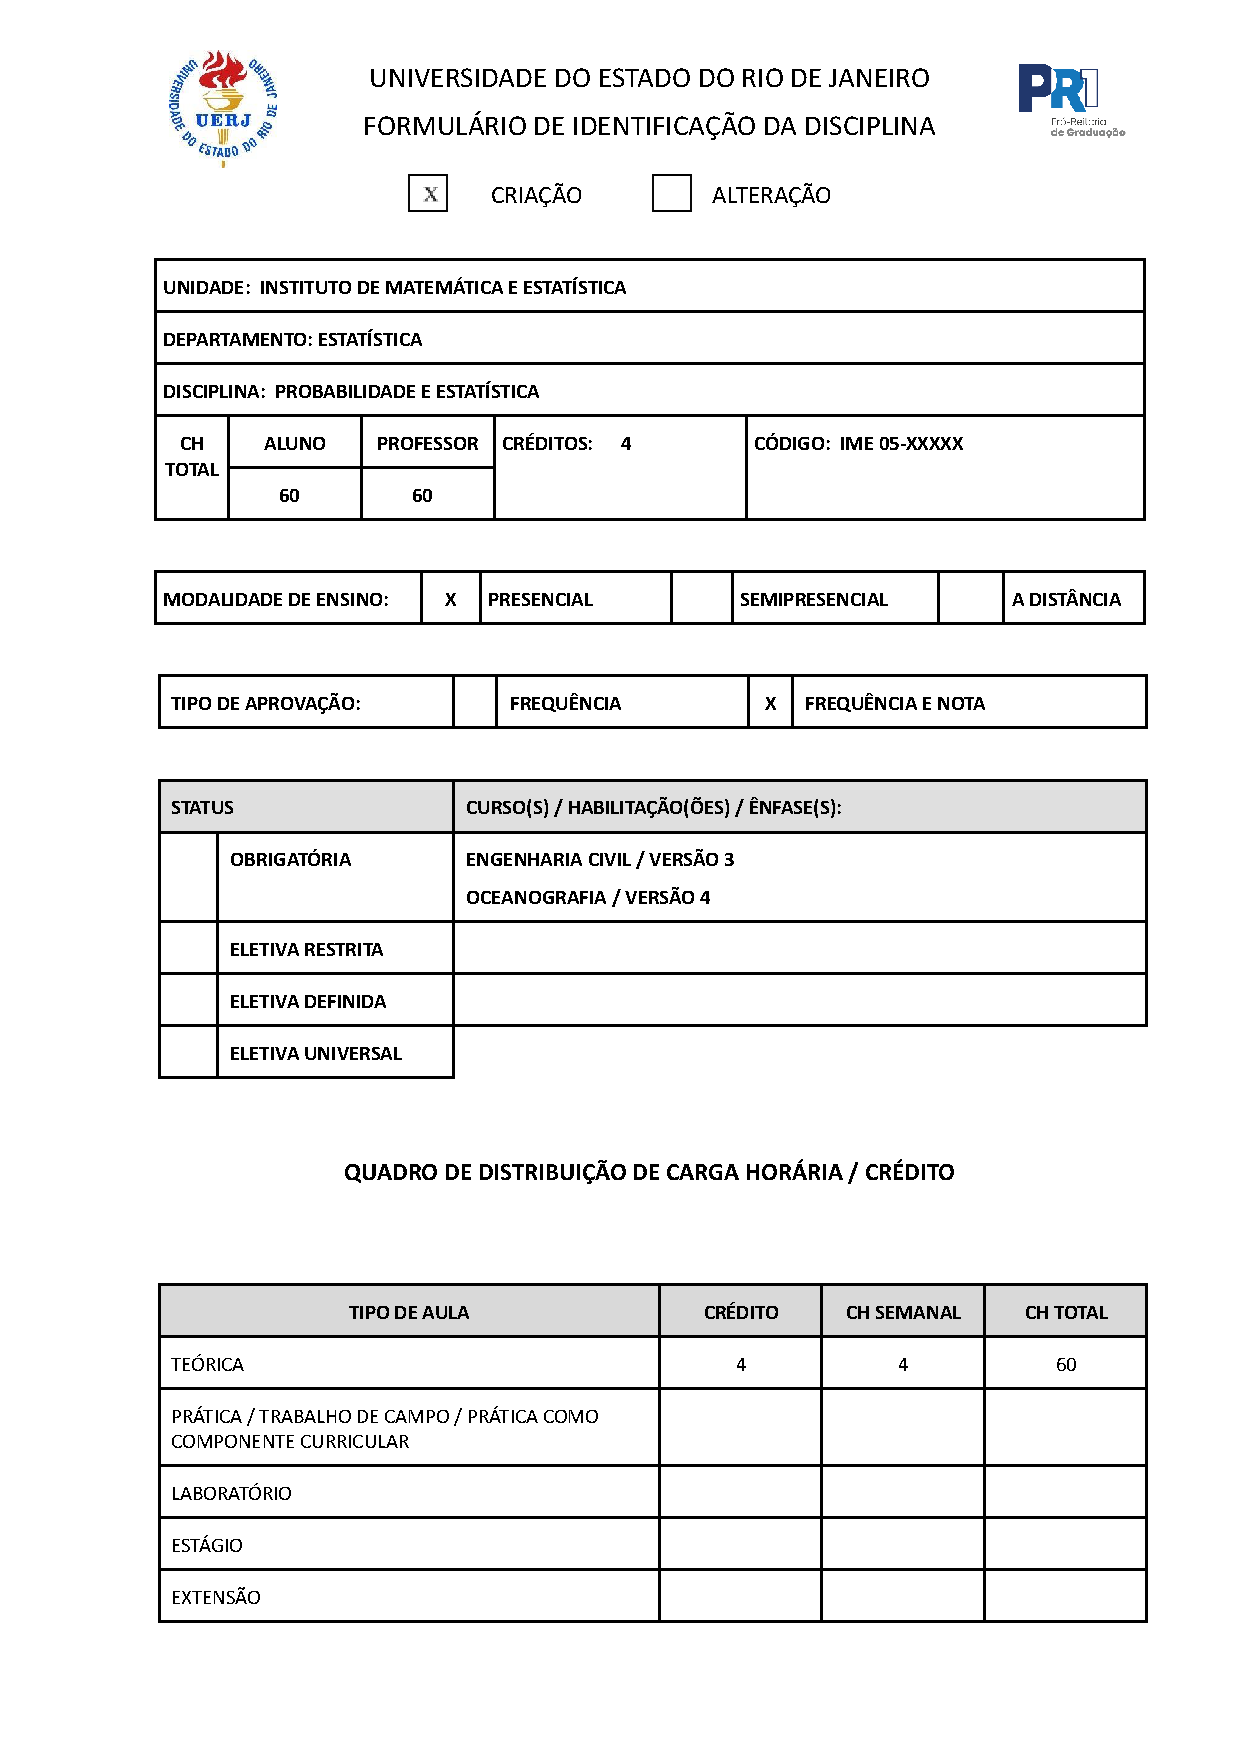
\includepdf[pages=-,addtotoc={1,section,1,{\ProbEst},},pagecommand={\thispagestyle{fancy}}]{ementasExternas/Probabilidade_e_Estatistica.pdf}
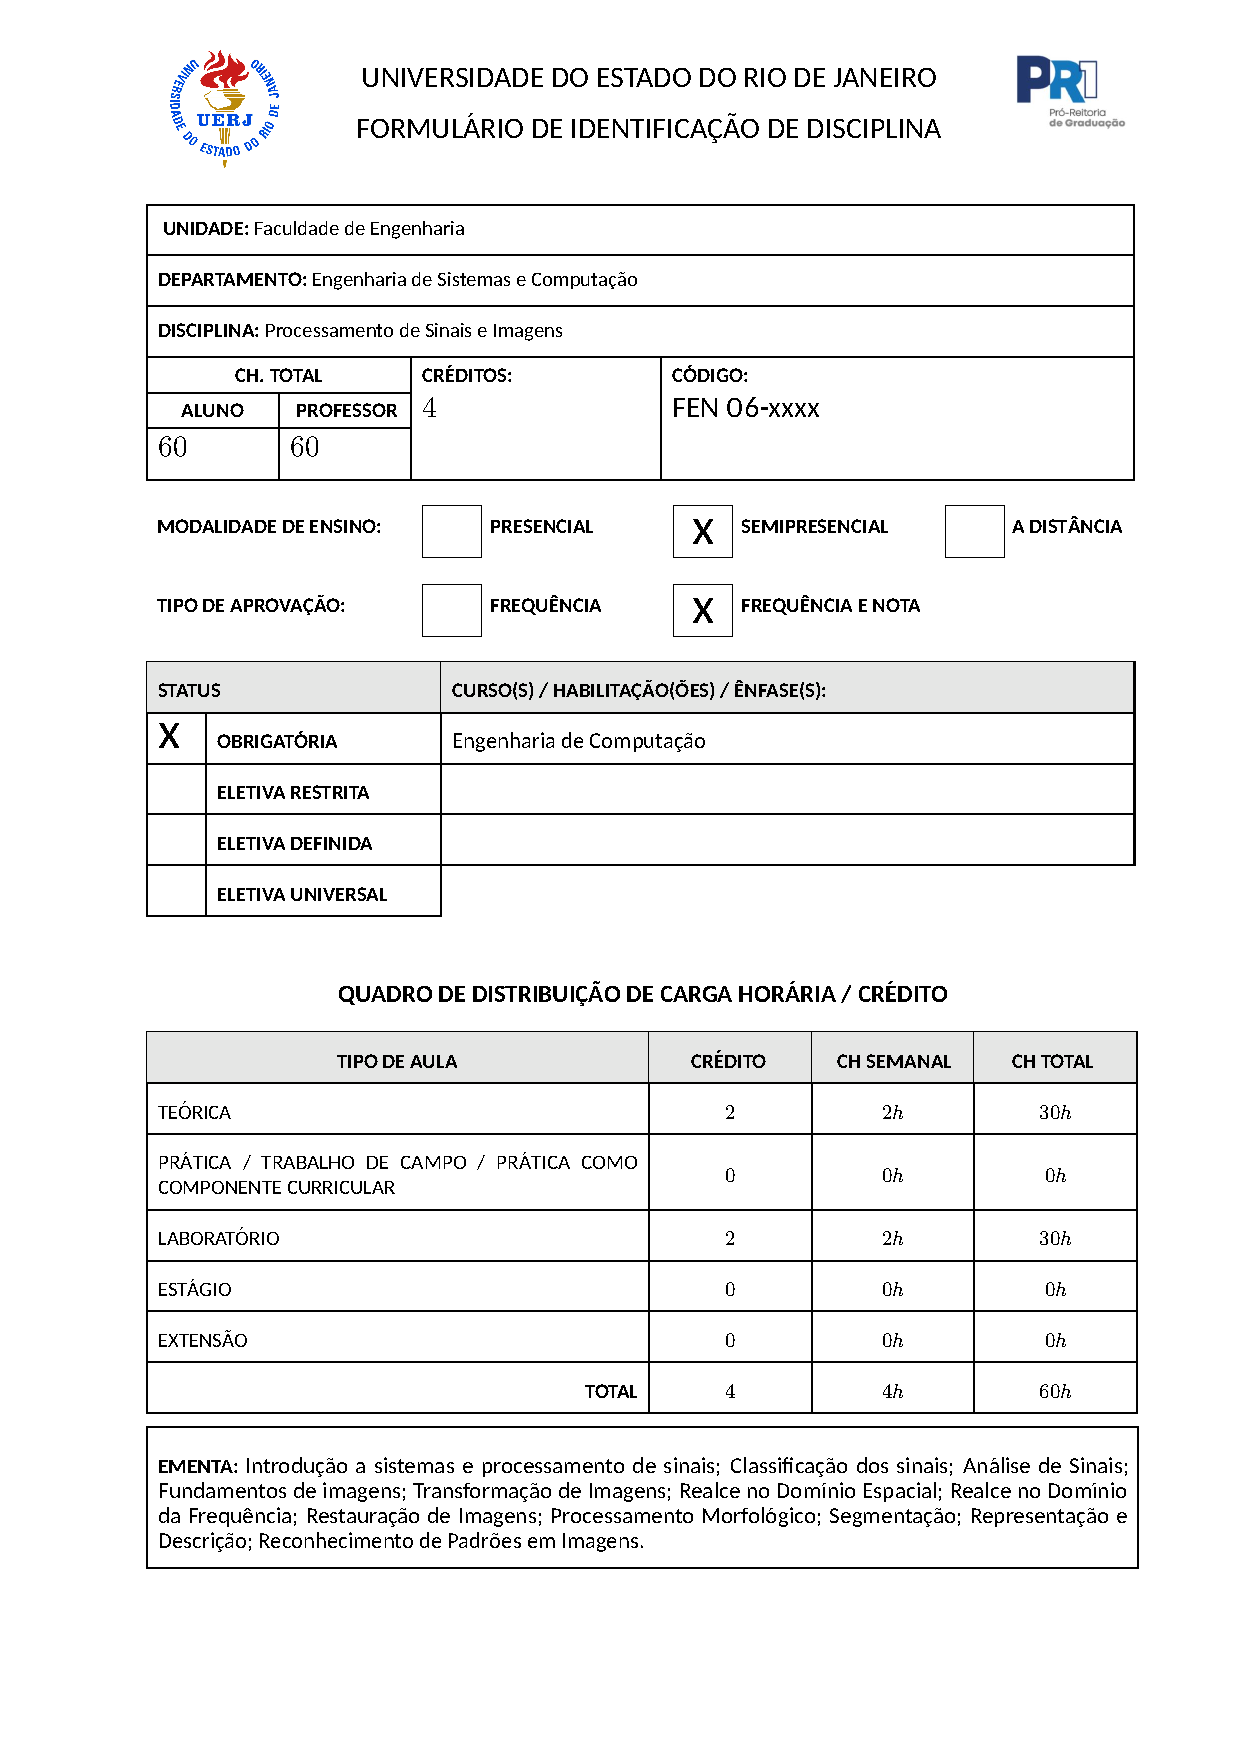
\includepdf[pages=-,addtotoc={1,section,1,{\ProcImag},},pagecommand={\thispagestyle{fancy}}]{ementas/ProcessamentoDeImagens.pdf}
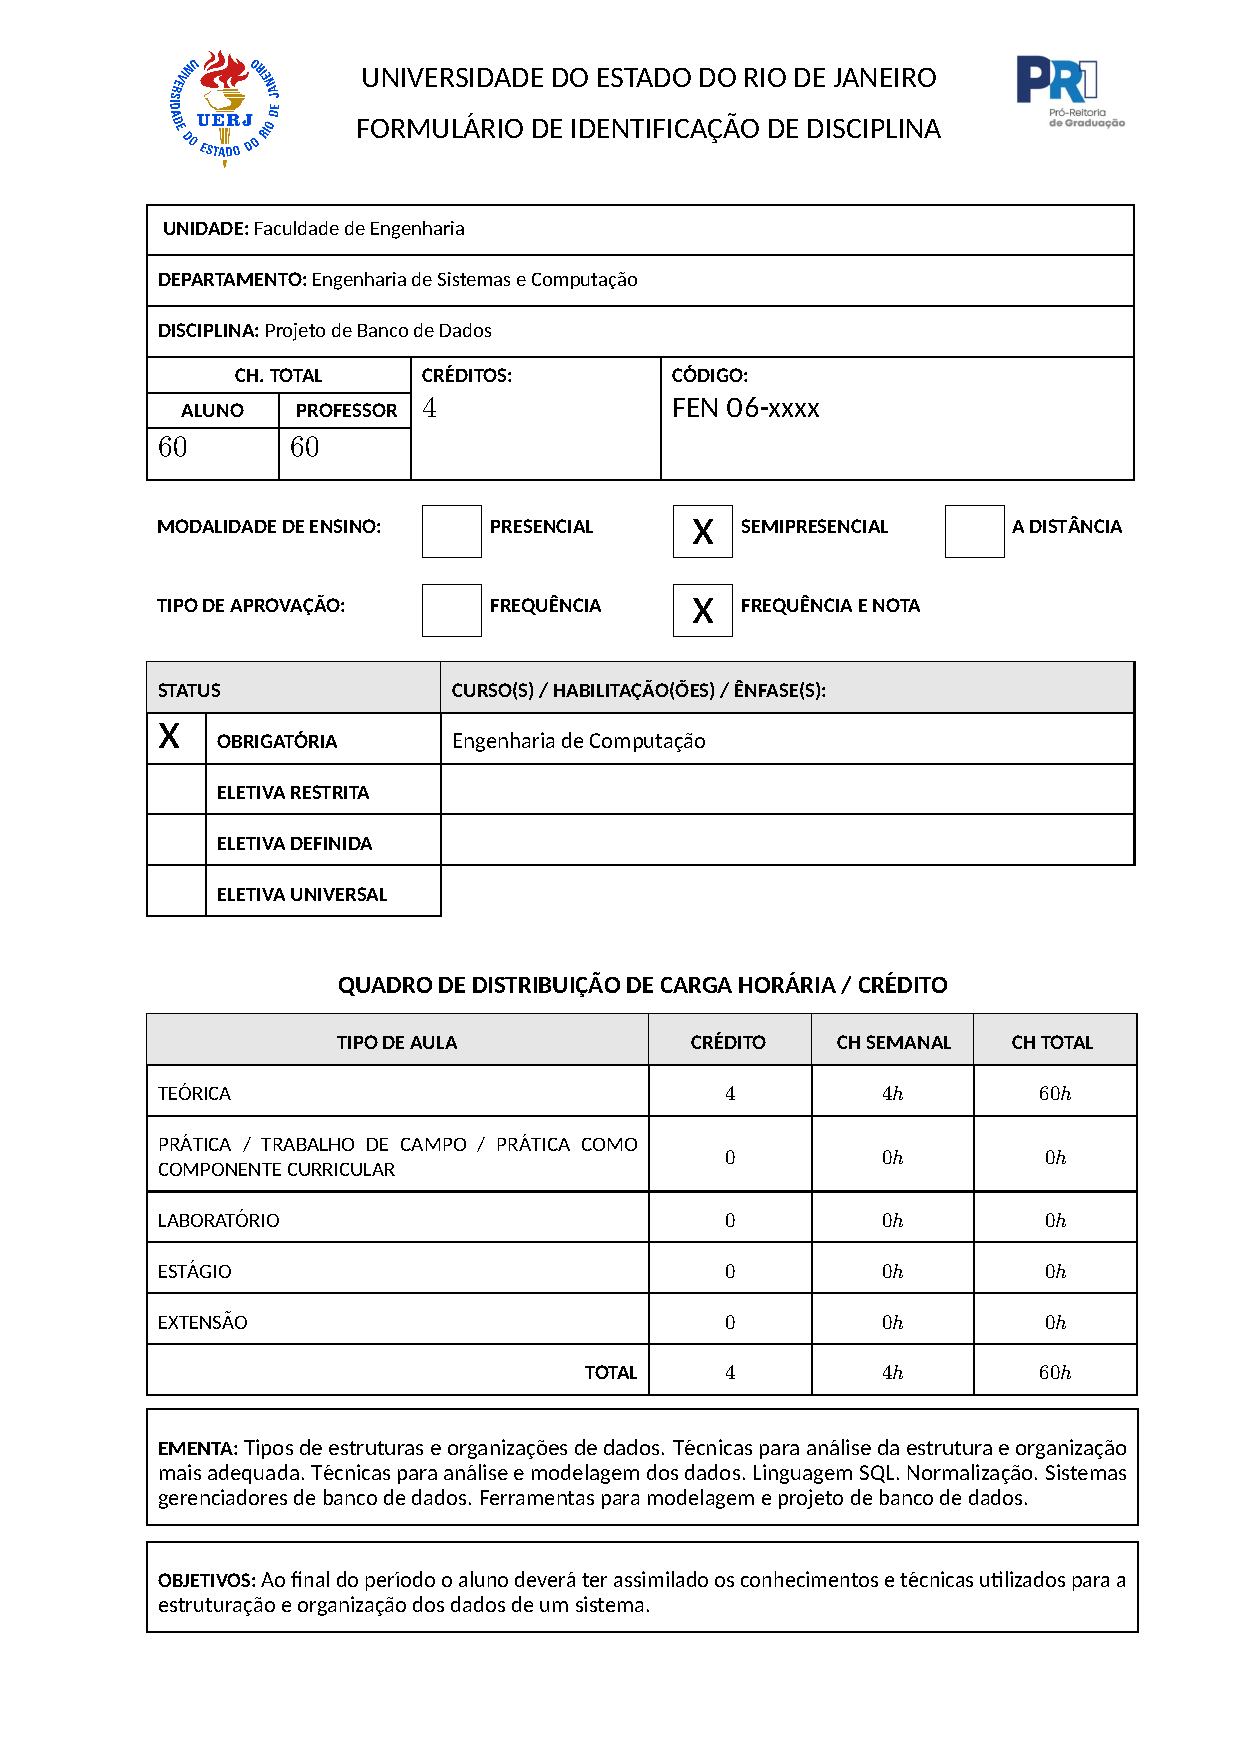
\includepdf[pages=-,addtotoc={1,section,1,{\ProjBD},},pagecommand={\thispagestyle{fancy}}]{ementas/ProjetoEAdministracaoDeBancoDeDados.pdf}
% Projetos de Extensão
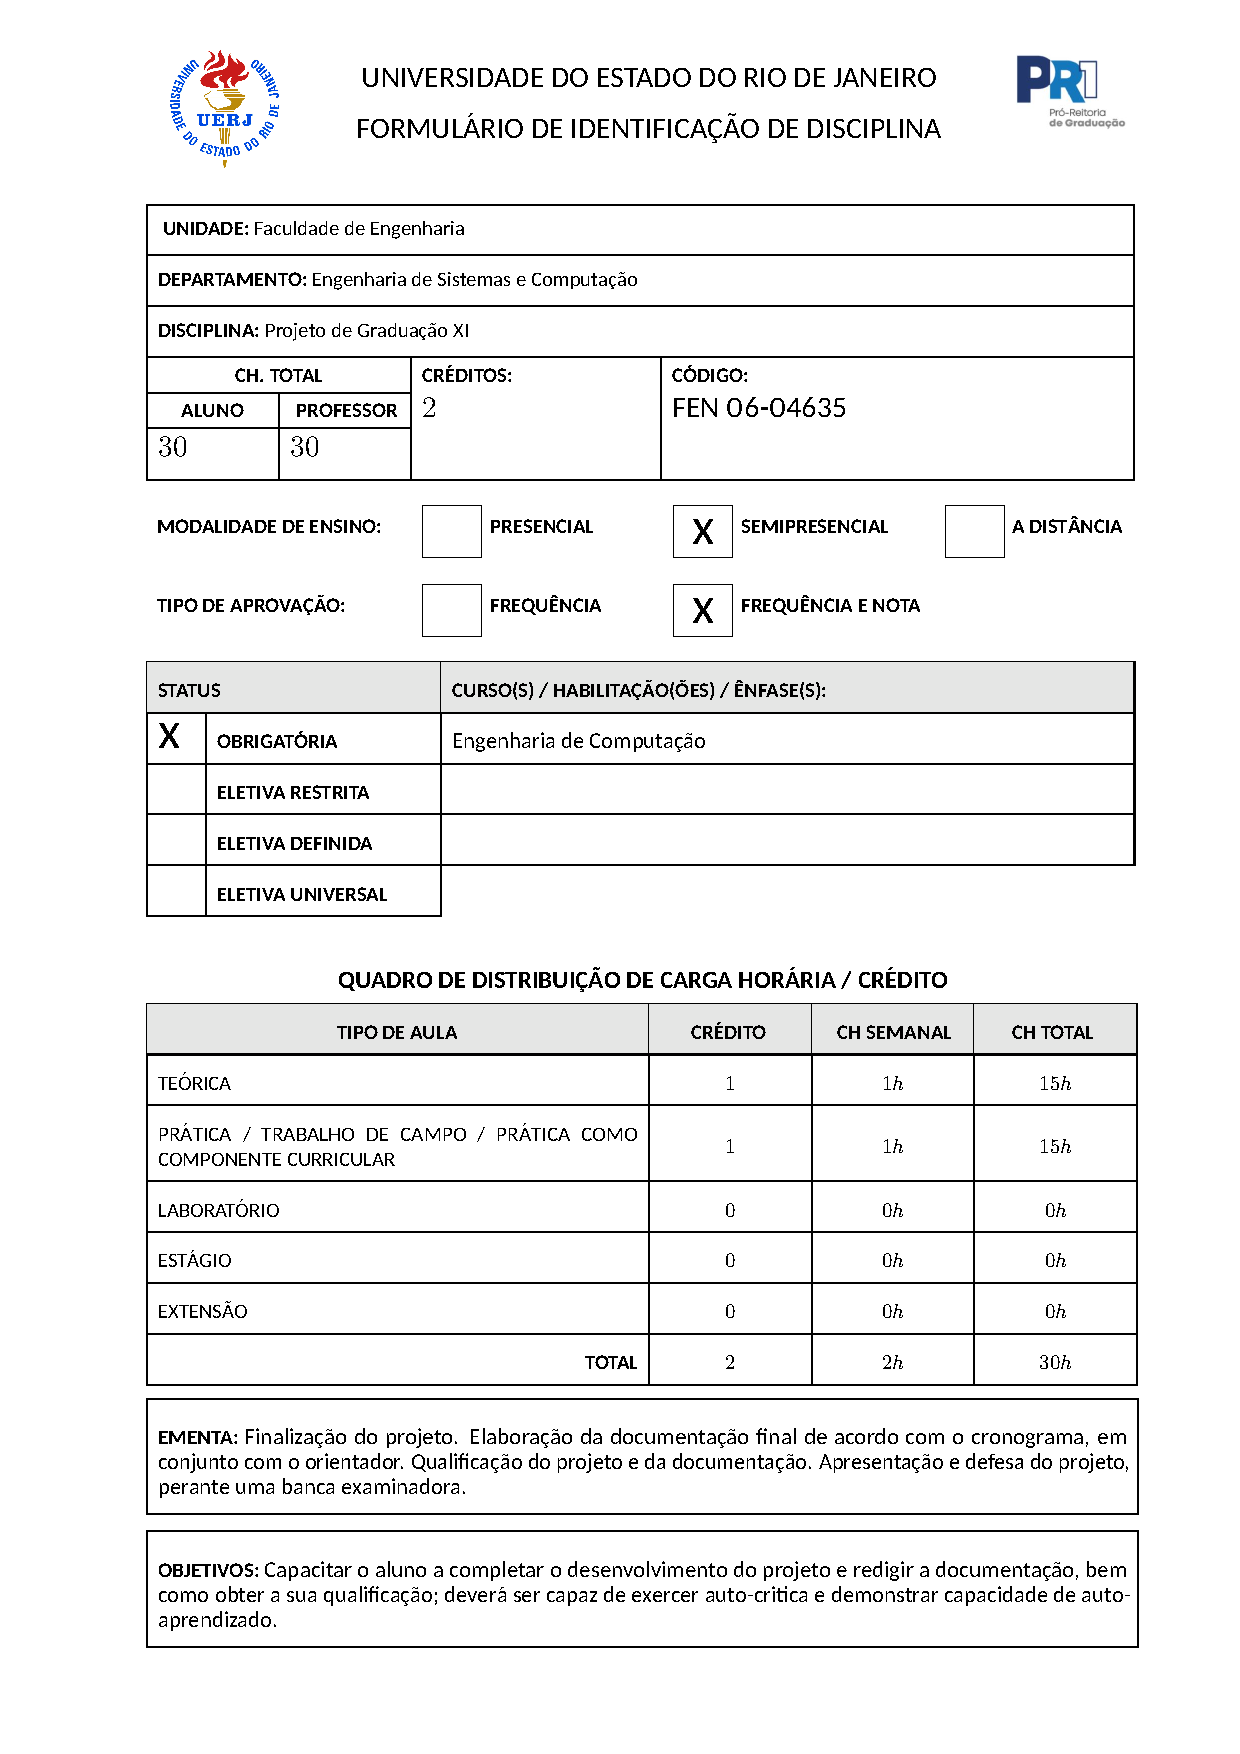
\includepdf[pages=-,addtotoc={1,section,1,{\ProjB},},pagecommand={\thispagestyle{fancy}}]{ementas/ProjetoXIB.pdf}
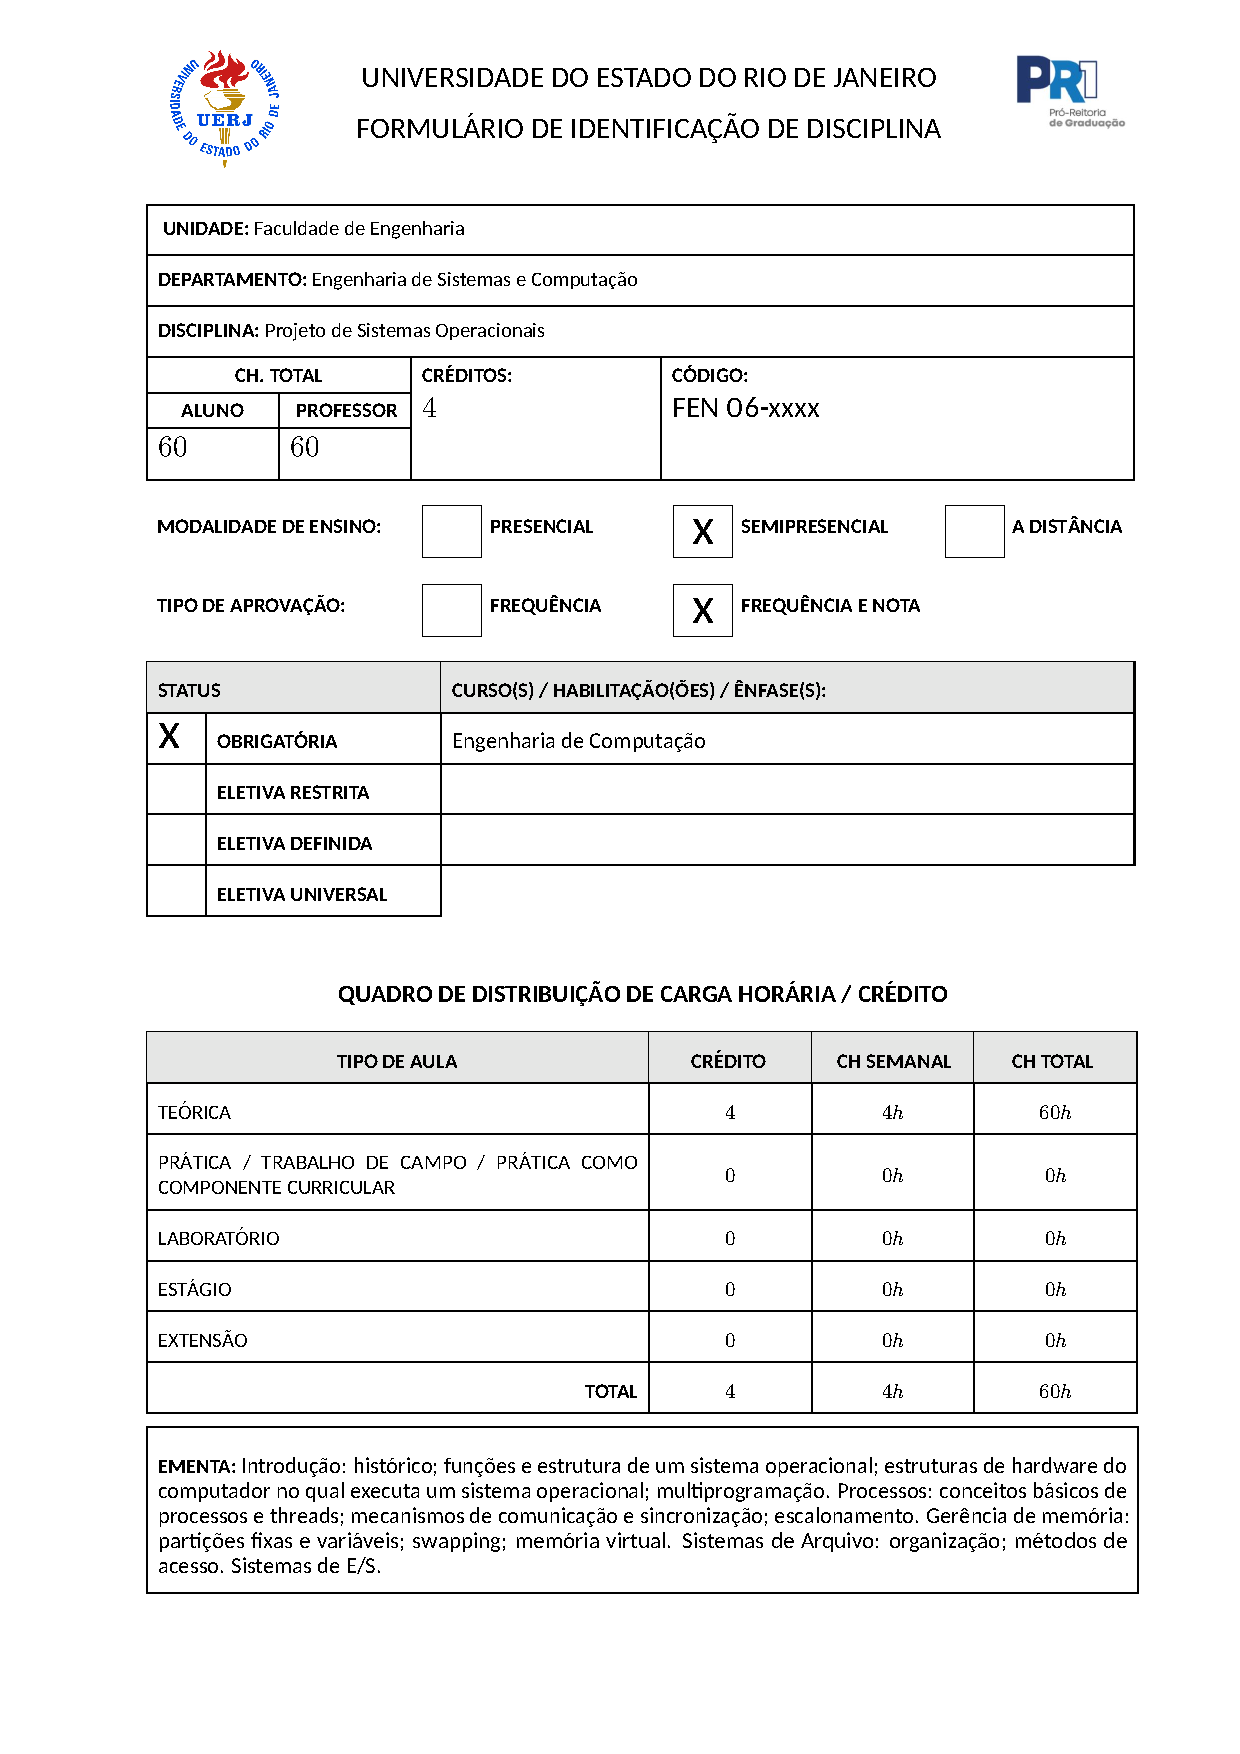
\includepdf[pages=-,addtotoc={1,section,1,{\ProjSO},},pagecommand={\thispagestyle{fancy}}]{ementas/ProjetoDeSistemasOperacionais.pdf}
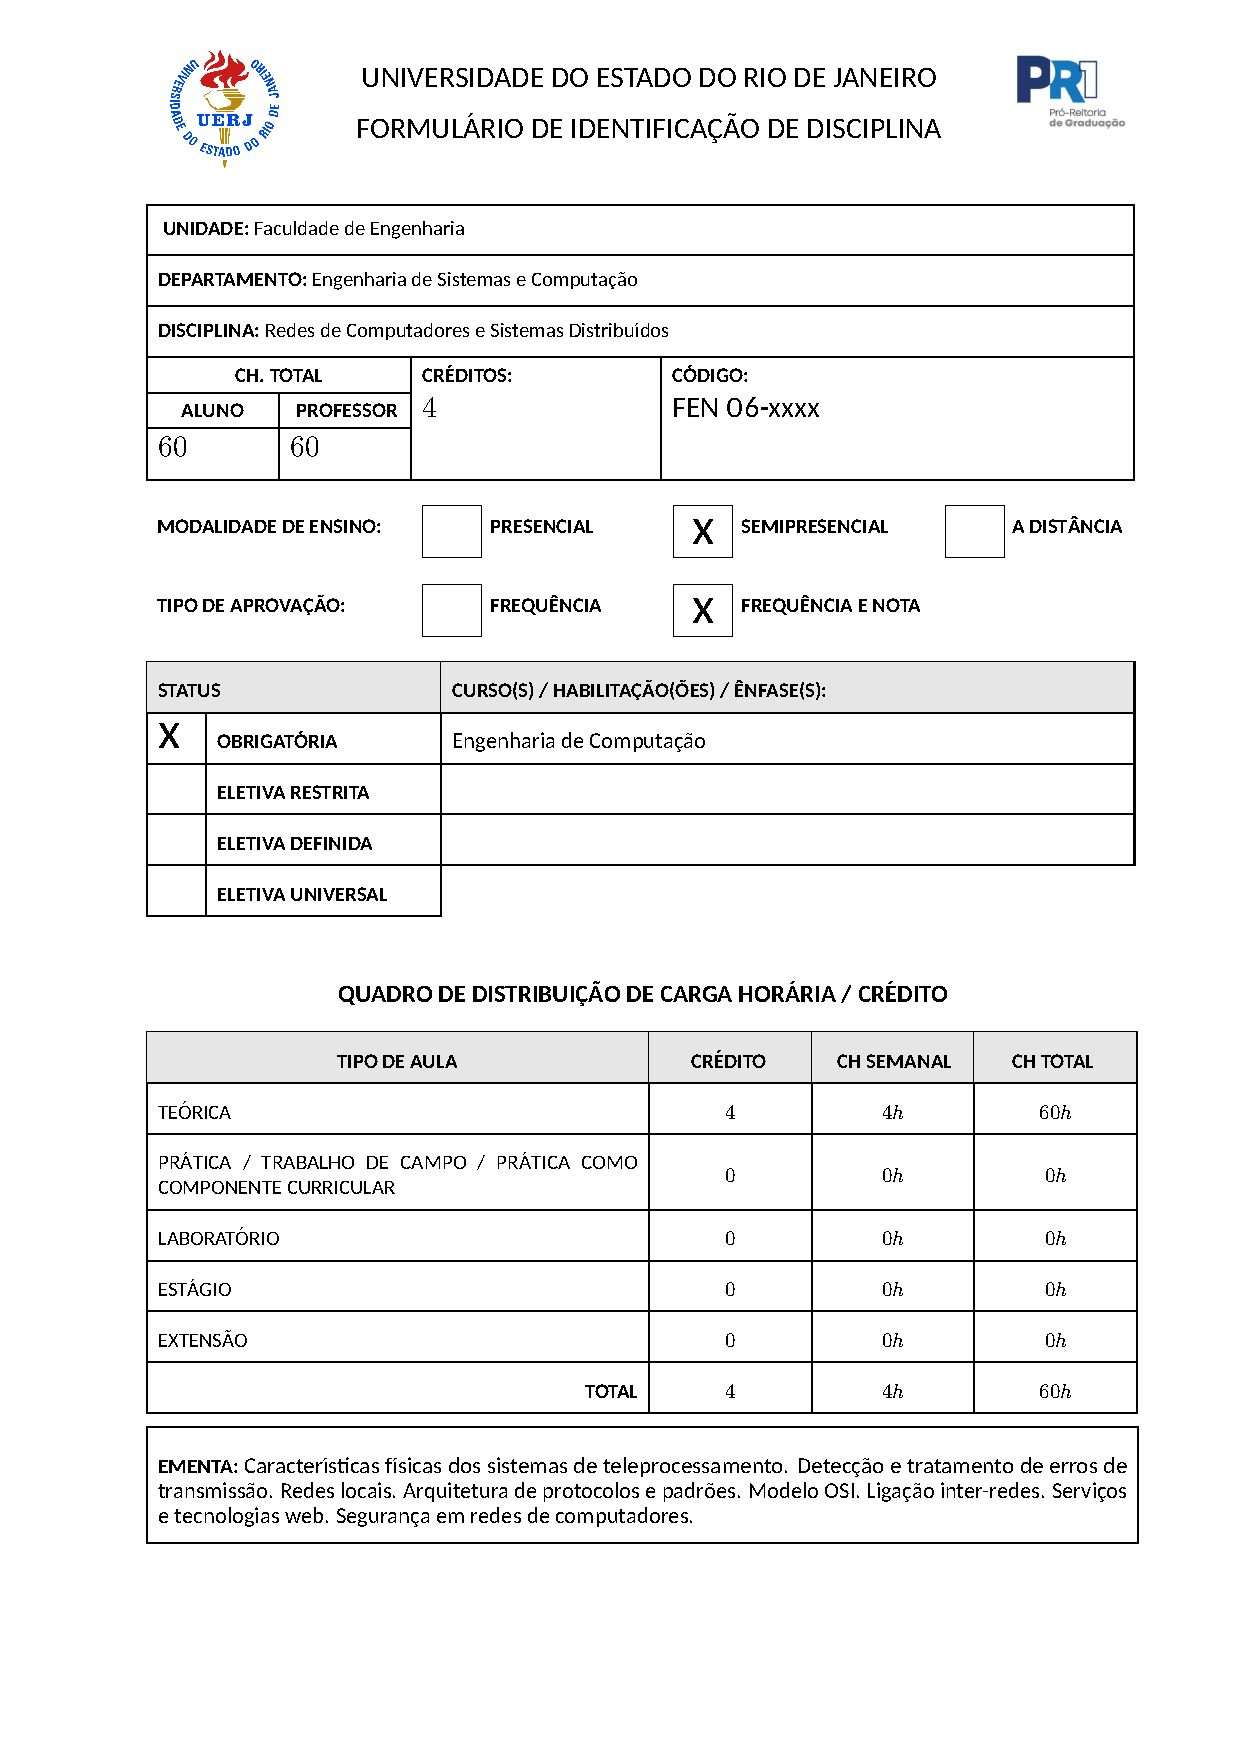
\includepdf[pages=-,addtotoc={1,section,1,{\Telep},},pagecommand={\thispagestyle{fancy}}]{ementas/TeleprocessamentoERedes.pdf} % Redes de Computadores e Sistemas Distribuídos
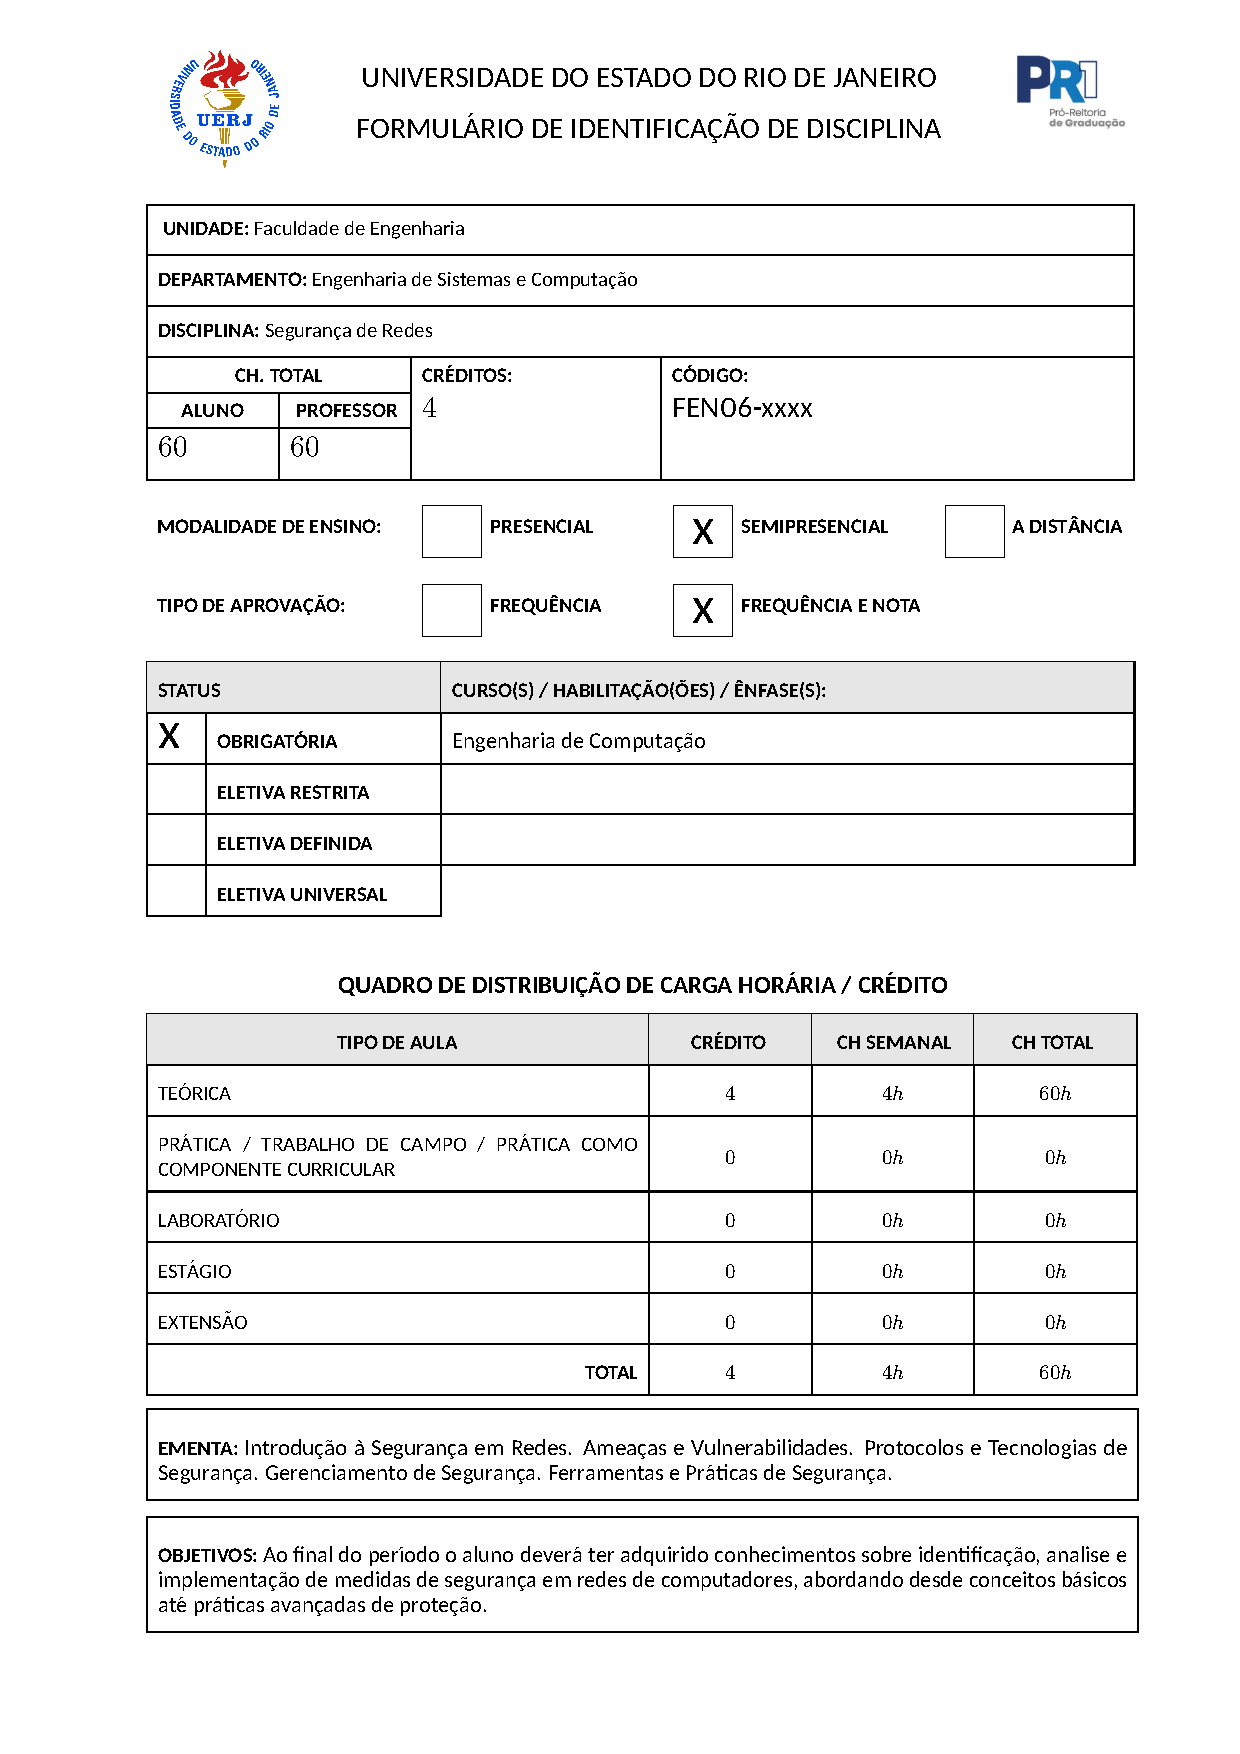
\includepdf[pages=-,addtotoc={1,section,1,{\Sredes},},pagecommand={\thispagestyle{fancy}}]{ementas/seguranca_de_redes.pdf}
% Sinais e Sistemas
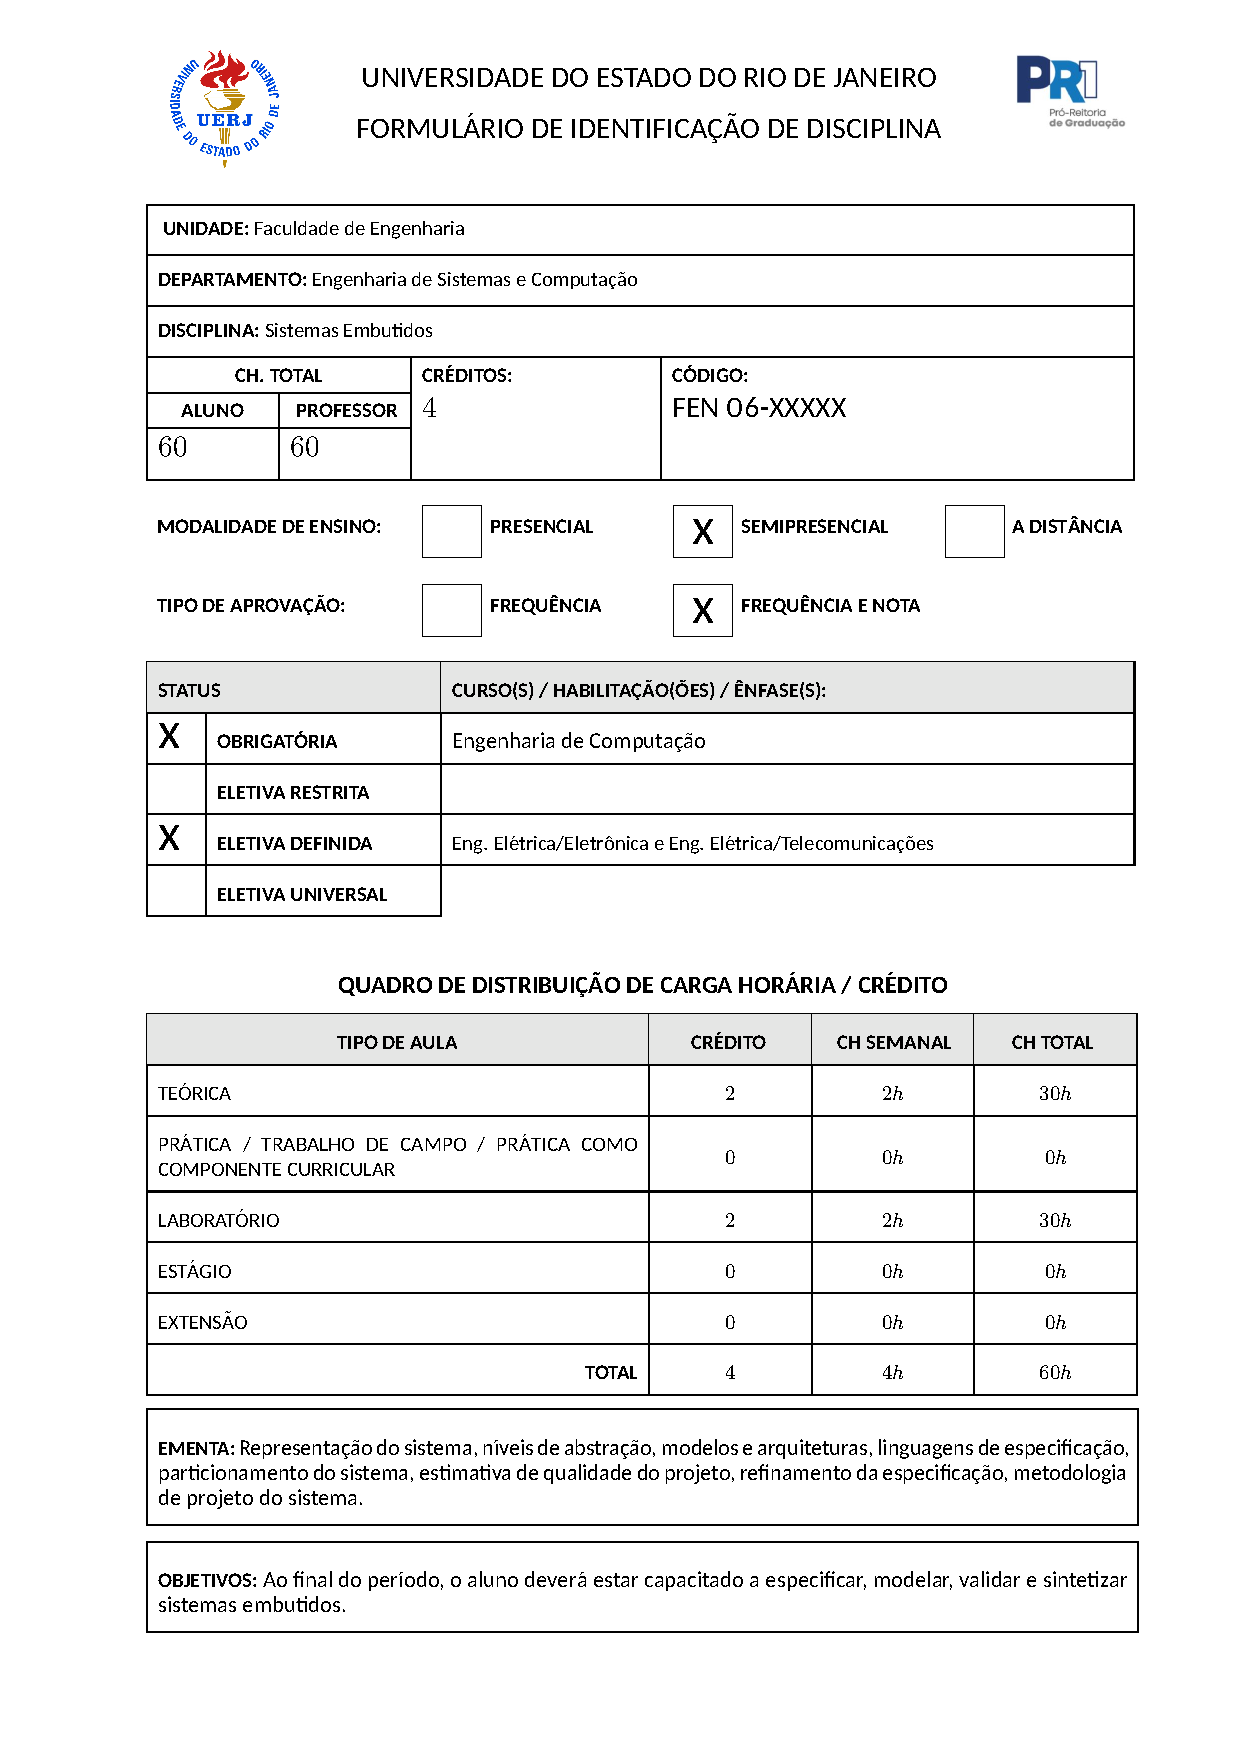
\includepdf[pages=-,addtotoc={1,section,1,{\SistEmb},},pagecommand={\thispagestyle{fancy}}]{ementas/SistemasEmbutidos.pdf}
% Técnicas Digitais
\includepdf[pages=-,addtotoc={1,section,1,{\TeoComp},},pagecommand={\thispagestyle{fancy}}]{ementas/TeoriaDeCompiladores.pdf}
\includepdf[pages=-,addtotoc={1,section,1,{\Grafos},},pagecommand={\thispagestyle{fancy}}]{ementas/TeoriadosGrafos.pdf}


\chapter{Ementas de Disciplinas Eletivas}
% \includepdf[pages=-,addtotoc={1,section,1,{\EletRec},},pagecommand={\thispagestyle{fancy}}]{Eletiva1_ReconhecimentoDePadroes.pdf}
% Aprendizado por Reforço
\includepdf[pages=-,addtotoc={1,section,1,{\EletReforco},},pagecommand={\thispagestyle{fancy}}]{ementas/eletiva_aprendizado_por_reforco.pdf}
% Processamento de Linguagem Natural
\includepdf[pages=-,addtotoc={1,section,1,{\AprendProfPLN},},pagecommand={\thispagestyle{fancy}}]{ementas/eletiva_NLP.pdf}
% Aprendizado Profundo para Visão Computacional
\includepdf[pages=-,addtotoc={1,section,1,{\EletVisao},},pagecommand={\thispagestyle{fancy}}]{ementas/eletiva_visao_computacional.pdf}
% Automação de Processos Robóticos
\includepdf[pages=-,addtotoc={1,section,1,{\AutomProcRob},},pagecommand={\thispagestyle{fancy}}]{ementas/eletiva_automacao_processos_roboticos.pdf}
% Arquiteturas Avançadas de Computadores
\includepdf[pages=-,addtotoc={1,section,1,{\EletArq},},pagecommand={\thispagestyle{fancy}}]{ementas/Eletiva4_ComputacaoDeAltoDesempenho.pdf}
% Geomática
\includepdf[pages=-,addtotoc={1,section,1,{\EletGeo},},pagecommand={\thispagestyle{fancy}}]{ementas/Eletiva3_Geomatica.pdf}
% Redes de Interconexão
\includepdf[pages=-,addtotoc={1,section,1,{\EletRedes},},pagecommand={\thispagestyle{fancy}}]{ementas/Eletiva2_RedesDeInterconexao.pdf}
% Sistemas Operacionais para Robótica Inteligente
\includepdf[pages=-,addtotoc={1,section,1,{\SistOpRobInt},},pagecommand={\thispagestyle{fancy}}]{ementas/eletiva_ROS.pdf}
% Técnicas de Programação em Otimização Combinatória
\includepdf[pages=-,addtotoc={1,section,1,{\TecProgOtim},},pagecommand={\thispagestyle{fancy}}]{ementas/eletiva_tecnicas_de_programacao_em_otimizacao_combinatoria.pdf}
% Tópicos Especiais em Visão Computacional

% Legislação
\includepdf[pages=-,addtotoc={1,section,1,{\TopEspVisComp},},pagecommand={\thispagestyle{fancy}}]{ementas/eletiva_topicos_especiais_em_visao_computacional.pdf}
% Institui as Diretrizes Curriculares Nacionais para os cursos de graduação na área da Computação
\chapter{Resolução CNE/CES n\textordmasculine{} 5, de 16 de novembro de 2016}
\label{cne2016}
\includepdf[pages=-,pagecommand={\thispagestyle{fancy}}]{leis/rces005_16.pdf}
% Referenciais SBC para cursos de Computação
\chapter{SBC: Referenciais para Graduação em Computação}
\label{sbc2017}
\includepdf[pages=-,pagecommand={\thispagestyle{fancy}}]{leis/sbc2017.pdf}
% Resolução CNE/CES n. 7/2018, que estabelece as as Diretrizes para a Extensão na Educação Superior Brasileira
\chapter{RESOLUÇÃO N\textordmasculine{} 7, DE 18 DE DEZEMBRO DE 2018 - CNE/CES}
\label{rcne2018}
\includepdf[pages=-,pagecommand={\thispagestyle{fancy}}]{leis/rces007_18.pdf}
% Deliberação n. 33/95, regras gerais de graduação UERJ
\chapter{Deliberação n\textordmasculine{} 33/95 da UERJ}
\label{delib3395}
\includepdf[pages=-,pagecommand={\thispagestyle{fancy}}]{leis/del-uerj1995.pdf}
% Deliberação n. 59/2019 da UERJ que altera a Deliberação n. 33/95 
\chapter{Deliberação n\textordmasculine{} 59/2019 da UERJ}
\label{delib592019}
\includepdf[pages=-,pagecommand={\thispagestyle{fancy}}]{leis/del-uerj2019.pdf}
%  Resolução n. 380/1993 CREA/CONFEA. Discrimina as atribuições do Engenheiro de Computação
\chapter{Resolução n\textordmasculine{} 380/1993 CREA/CONFEA}
\label{confea1993}
\includepdf[pages=1,pagecommand={\thispagestyle{fancy}}]{leis/confea93.pdf}
% Deliberaçao n. 2/2023 do CSEPE/UERJ dispõe sobre inserção curricular da extensão na UERJ
\chapter{Deliberação n\textordmasculine{} 4/2023 do CSEPE/UERJ}
\label{del4}
\includepdf[pages=-,pagecommand={\thispagestyle{fancy}}]{leis/del-uerj2023.pdf}

% Acrescenta os apêndices ao sumário
\addappheadtotoc
\end{document}
